%%% Dokumentenklasse
\documentclass[10pt,a4paper,draft=false]{scrreprt}
\KOMAoption{toc}{listof,bib}

%%% Kopf & Fußzeile
\usepackage[
automark,			%automatische Aktualisierung des Kolumnentitels in der Kopfzeile
headsepline,		%Strich UNTER der Kopfzeile
footsepline			%Strich ÜBER der Fußzeile
]{scrpage2}

%%% Sprach Pakete
\usepackage[ngerman]{babel}
%\usepackage[ansinew]{inputenc} % Falls es Probleme mit ä,ö,ü ... gibt, sollte das Packet in dieser Zeile wieder aktiviert werden 
\usepackage[utf8]{inputenc} % wenn der Kommentar aus der oberen Zeile entfehrnt wird, muss diese Zeile kommentiert werden
\usepackage[babel, german=quotes]{csquotes}
\usepackage[T1]{fontenc}

%%% Style Packete
\usepackage{geometry}
\usepackage{graphicx}
\usepackage{textcomp}
\usepackage{float}
\usepackage{longtable} 	
\usepackage{tabularx}
\usepackage{ltablex} % kombiniert longtable und tabularx; benötigt den befehl \keepXColumns direkt vor \begin{tabularx} damit der X-Character der spalten erhalten bleibt
\usepackage{multirow,array,booktabs} 
\usepackage[bf, flushleft,justification=justified]{caption}[2018/05/01] 
\usepackage{subcaption}
\usepackage{threeparttable}
\usepackage{upgreek} % Nicht kursive Griechische Buchstaben einbinden
\usepackage{textgreek} % For greek letters in the text

% Hyperref: Klickbare Verweise in PDF-Dokumenten bei Verwendung von pdftex.
%           Einstellbare Optionen für die PDF-Dokumenteigenschaften:
%           - pdftitle:  Titel des Dokuments
%           - pdfauthor: Autor der Arbeit
%           ACHTUNG: Leerzeichen sind in den Optionen nicht zulässig. Am
%           besten geschützte Leerzeichen (~) benutzen.
\usepackage[colorlinks=true,citecolor=red]{hyperref}

%%% Mathematik Packete
\usepackage{amsfonts}
\usepackage{amssymb}
\usepackage{setspace}
\usepackage{amsmath}
\usepackage[amssymb]{SIunits} % Einbinden von SI - Einheiten

%Chemie Packete
\usepackage{chemmacros}
\usepackage{chemformula}
\usepackage{chemfig}

%%% Abkürzungen
\usepackage[printonlyused,withpage]{acronym}

%%% Spaltentypen in Tabellen (mit dem Packet "tabularx")
\usepackage{array}
\newcolumntype{L}{>{\raggedright\arraybackslash}X} % linksbündig mit Breitenangabe
\newcolumntype{C}{>{\centering\arraybackslash}X} % zentriert mit Breitenangabe
\newcolumntype{R}{>{\raggedleft\arraybackslash}X} % rechtsbündig mit Breitenangabe

%%% Bibliografie
\usepackage[
backend=biber,
sorting=none,
style=numeric-comp,    		   % Zitierstil
isbn=false,     % isbn nicht anzeigen, gleiches geht mit nahezu allen anderen Feldern
url=false,		%url wird nicht angezeigt
doi=false,		%doi wird angezeigt
eprint=false,	%eprint wird nicht angezeigt
pagetracker=true,          % ebd. bei wiederholten Angaben (false=ausgeschaltet, page=Seite, spread=Doppelseite, true=automatisch)
ibidtracker=true,
maxbibnames=50,            % maximale Namen, die im Literaturverzeichnis angezeigt werden (ich wollte alle)
maxcitenames=3,            % maximale Namen, die im Text angezeigt werden, ab 4 wird u.a. nach den ersten Autor angezeigt
autocite=inline,           % regelt Aussehen für \autocite (inline=\parancite)
block=space,               % kleiner horizontaler Platz zwischen den Feldern
backref=true,              % Seiten anzeigen, auf denen die Referenz vorkommt
backrefstyle=three+,       % fasst Seiten zusammen, z.B. S. 2f, 6ff, 7-10
date=short,                % Datumsformat
]{biblatex}
\setlength{\bibitemsep}{1em}     % Abstand zwischen den Literaturangaben
\setlength{\bibhang}{2em}        % Einzug nach jeweils erster Zeile

%--------------------------------------------------

% %% Bibliographie laden
\bibliography{Literatur/literatur.bib} 

%%% Kapitel einbinden
\includeonly{
%	Kapitel/01-Einleitung/einleitung,
%	Kapitel/02-Material-und-Methoden/material-und-methoden,
%	Kapitel/03-Ergebnisse/ergebnisse,
	Kapitel/04-Diskussion/diskussion,
	Kapitel/05-Fazit/fazit,
%	Kapitel/06-Ausblick/ausblick,
}
%--------------------------------------------------

\author{Julian Blaser}
\title{\Huge \textbf{Titel}}
\date{\today}

%------------Fancy Header------------------
%\pagestyle{fancy}
%\renewcommand{\sectionmark}[1]{\markboth{\emph{#1}}{}}
%\fancyhf{}

%\fancyhead[LE,RO]{\textbf{\thepage}}
%\fancyhead[LO,RE]{\textbf{\leftmark}}
%\fancyfoot[LE,RO]{\author{Julian Blaser}}
%\fancyfoot[LO,RE]{\date{\today}}
%\renewcommand{\headrulewidth}{0.5pt}
%\renewcommand{\footrulewidth}{0.5pt}
%----------Ende Fancy Header---------------


%%% ------------Kopf&Fußzeile KOMA Skript------------------
\pagestyle{scrheadings}

\ihead{\raisebox{1.mm}{\headmark}}
\ohead{\raisebox{1.mm}{\pagemark}}
\chead{}
\ofoot{\raisebox{-1.5mm}{Julian Blaser}}
\ifoot{\raisebox{-1.5mm}{Hochschule München}}
\cfoot{}

\setheadsepline{.5pt}
\setfootsepline{.5pt}

%%% ------------Kopf&Fußzeile KOMA Skript------------------

\setlength{\parindent}{0em} % Automatisches Einrücken nach Absatz verhindern

\begin{document}
	
	
% häufig benutzte Redewendungen
\newcommand{\abb}{Abbildung}
\newcommand{\abbn}{Abbildungen}
\newcommand{\spitze}{Abtastspitze}
\newcommand{\spitzen}{Abtastspitzen}
\newcommand{\amid}{Amidbindung}
\newcommand{\amide}{Amidbindungen}
\newcommand{\amino}{Aminogruppe}
\newcommand{\aminos}{Aminogruppen}
\newcommand{\carboxy}{Carboxylgruppe}
\newcommand{\carboxys}{Carboxylgruppen}
\newcommand{\spacer}{CMA-Spacer}
\newcommand{\spacers}{CMA-Spacers}	
\newcommand{\substrat}{DLC-Substrat}
\newcommand{\substrats}{DLC-Substrats}
\newcommand{\gl}{Gleichung}
\newcommand{\gln}{Gleichungen}
\newcommand{\ester}{NHS-Ester}
\newcommand{\estern}{NHS-Estern}
\newcommand{\samplerate}{Samplerate}
	
% häufig verwendete Zahlen
\newcommand{\hscaleZero}{1}
\newcommand{\hscaleOne}{0.75}
\newcommand{\hsclaeChemfig}{0.65}
\newcommand{\hscaleTwo}{0.5}

% text für fußnoten etc.
\newcommand{\noteOne}{text}
\newcommand{\noteTwo}{text}
\newcommand{\noteThree}{text}
\newcommand{\noteFour}{text}
	
	\pagenumbering{Roman}%----------------------------------------

%	Titelseite
	%%%%%%%%%%%%%%%%%%%%%%%%%%%%%%%%%%%%%%%%%
% University Assignment Title Page 
% LaTeX Template
% Version 1.0 (27/12/12)
%
% This template has been downloaded from:
% http://www.LaTeXTemplates.com
%
% Original author:
% WikiBooks (http://en.wikibooks.org/wiki/LaTeX/Title_Creation)
%
% License:
% CC BY-NC-SA 3.0 (http://creativecommons.org/licenses/by-nc-sa/3.0/)
% 
% Instructions for using this template:
% This title page is capable of being compiled as is. This is not useful for 
% including it in another document. To do this, you have two options: 
%
% 1) Copy/paste everything between \begin{document} and \end{document} 
% starting at \begin{titlepage} and paste this into another LaTeX file where you 
% want your title page.
% OR
% 2) Remove everything outside the \begin{titlepage} and \end{titlepage} and 
% move this file to the same directory as the LaTeX file you wish to add it to. 
% Then add %%%%%%%%%%%%%%%%%%%%%%%%%%%%%%%%%%%%%%%%%
% University Assignment Title Page 
% LaTeX Template
% Version 1.0 (27/12/12)
%
% This template has been downloaded from:
% http://www.LaTeXTemplates.com
%
% Original author:
% WikiBooks (http://en.wikibooks.org/wiki/LaTeX/Title_Creation)
%
% License:
% CC BY-NC-SA 3.0 (http://creativecommons.org/licenses/by-nc-sa/3.0/)
% 
% Instructions for using this template:
% This title page is capable of being compiled as is. This is not useful for 
% including it in another document. To do this, you have two options: 
%
% 1) Copy/paste everything between \begin{document} and \end{document} 
% starting at \begin{titlepage} and paste this into another LaTeX file where you 
% want your title page.
% OR
% 2) Remove everything outside the \begin{titlepage} and \end{titlepage} and 
% move this file to the same directory as the LaTeX file you wish to add it to. 
% Then add %%%%%%%%%%%%%%%%%%%%%%%%%%%%%%%%%%%%%%%%%
% University Assignment Title Page 
% LaTeX Template
% Version 1.0 (27/12/12)
%
% This template has been downloaded from:
% http://www.LaTeXTemplates.com
%
% Original author:
% WikiBooks (http://en.wikibooks.org/wiki/LaTeX/Title_Creation)
%
% License:
% CC BY-NC-SA 3.0 (http://creativecommons.org/licenses/by-nc-sa/3.0/)
% 
% Instructions for using this template:
% This title page is capable of being compiled as is. This is not useful for 
% including it in another document. To do this, you have two options: 
%
% 1) Copy/paste everything between \begin{document} and \end{document} 
% starting at \begin{titlepage} and paste this into another LaTeX file where you 
% want your title page.
% OR
% 2) Remove everything outside the \begin{titlepage} and \end{titlepage} and 
% move this file to the same directory as the LaTeX file you wish to add it to. 
% Then add \input{./title_page_1.tex} to your LaTeX file where you want your
% title page.
%
%%%%%%%%%%%%%%%%%%%%%%%%%%%%%%%%%%%%%%%%%

%----------------------------------------------------------------------------------------
%	PACKAGES AND OTHER DOCUMENT CONFIGURATIONS
%----------------------------------------------------------------------------------------

\begin{titlepage}

\newcommand{\HRule}{\rule{\linewidth}{0.5mm}} % Defines a new command for the horizontal lines, change thickness here

\center % Center everything on the page
 
%----------------------------------------------------------------------------------------
%	HEADING SECTIONS
%----------------------------------------------------------------------------------------

\textsc{\LARGE Hochschule München}\\[1.5cm] % Name of your university/college
\textsc{\Large Fakultät für Angewandte Naturwissenschaften und Mechatronik}\\[0.5cm] % Major heading such as course name
%\textsc{\large Minor Heading}\\[0.5cm] % Minor heading such as course title

%----------------------------------------------------------------------------------------
%	TITLE SECTION
%----------------------------------------------------------------------------------------
\begin{spacing}{2}
\HRule \\[0.4cm]
{ \huge \bfseries Rasterkraftmikroskopische Untersuchungen zur pH-Abhängigkeit kovalenter Bindungen}\\[0.4cm] % Title of your document
\HRule \\[1.5cm]
 \end{spacing}
%----------------------------------------------------------------------------------------
%	AUTHOR SECTION
%----------------------------------------------------------------------------------------

\begin{minipage}{0.45\textwidth}
\begin{flushleft} \large
\emph{Autor:}\\
Julian \textsc{Blaser} % Your name
\end{flushleft}
\end{minipage}
~
\begin{minipage}{0.45\textwidth}
\begin{flushright} \large
\emph{Betreuer:} \\
Dr.~Hauke~\textsc{Clausen-Schaumann} \\ % Supervisor's Name
% Second Supervisor's Name
\end{flushright}
\end{minipage}\\[3,5cm]

% If you don't want a supervisor, uncomment the two lines below and remove the section above
%\Large \emph{Author:}\\
%John \textsc{Smith}\\[3cm] % Your name

%----------------------------------------------------------------------------------------
%	DATE SECTION
%----------------------------------------------------------------------------------------

{\large \today}\\[2,5cm] % Date, change the \today to a set date if you want to be precise

%----------------------------------------------------------------------------------------
%	LOGO SECTION
%----------------------------------------------------------------------------------------
\begin{figure}[H]
	\begin{subfigure}[b]{0.5\textwidth}
		\begin{flushleft}
		\scalebox{0.5}{
		
\includegraphics[width=\textwidth]{Abbildungen/Titellogo/HMlogo}
		}
		\end{flushleft}
	\end{subfigure}
	\begin{subfigure}[b]{0.5\textwidth}
		\begin{flushright}
		\scalebox{0.2}{
		
\includegraphics[width=\textwidth]{Abbildungen/Titellogo/CANTERlogo2}
		}
		\end{flushright}
	\end{subfigure}

\end{figure}
%----------------------------------------------------------------------------------------

\vfill % Fill the rest of the page with whitespace

\end{titlepage} to your LaTeX file where you want your
% title page.
%
%%%%%%%%%%%%%%%%%%%%%%%%%%%%%%%%%%%%%%%%%

%----------------------------------------------------------------------------------------
%	PACKAGES AND OTHER DOCUMENT CONFIGURATIONS
%----------------------------------------------------------------------------------------

\begin{titlepage}

\newcommand{\HRule}{\rule{\linewidth}{0.5mm}} % Defines a new command for the horizontal lines, change thickness here

\center % Center everything on the page
 
%----------------------------------------------------------------------------------------
%	HEADING SECTIONS
%----------------------------------------------------------------------------------------

\textsc{\LARGE Hochschule München}\\[1.5cm] % Name of your university/college
\textsc{\Large Fakultät für Angewandte Naturwissenschaften und Mechatronik}\\[0.5cm] % Major heading such as course name
%\textsc{\large Minor Heading}\\[0.5cm] % Minor heading such as course title

%----------------------------------------------------------------------------------------
%	TITLE SECTION
%----------------------------------------------------------------------------------------
\begin{spacing}{2}
\HRule \\[0.4cm]
{ \huge \bfseries Rasterkraftmikroskopische Untersuchungen zur pH-Abhängigkeit kovalenter Bindungen}\\[0.4cm] % Title of your document
\HRule \\[1.5cm]
 \end{spacing}
%----------------------------------------------------------------------------------------
%	AUTHOR SECTION
%----------------------------------------------------------------------------------------

\begin{minipage}{0.45\textwidth}
\begin{flushleft} \large
\emph{Autor:}\\
Julian \textsc{Blaser} % Your name
\end{flushleft}
\end{minipage}
~
\begin{minipage}{0.45\textwidth}
\begin{flushright} \large
\emph{Betreuer:} \\
Dr.~Hauke~\textsc{Clausen-Schaumann} \\ % Supervisor's Name
% Second Supervisor's Name
\end{flushright}
\end{minipage}\\[3,5cm]

% If you don't want a supervisor, uncomment the two lines below and remove the section above
%\Large \emph{Author:}\\
%John \textsc{Smith}\\[3cm] % Your name

%----------------------------------------------------------------------------------------
%	DATE SECTION
%----------------------------------------------------------------------------------------

{\large \today}\\[2,5cm] % Date, change the \today to a set date if you want to be precise

%----------------------------------------------------------------------------------------
%	LOGO SECTION
%----------------------------------------------------------------------------------------
\begin{figure}[H]
	\begin{subfigure}[b]{0.5\textwidth}
		\begin{flushleft}
		\scalebox{0.5}{
		
\includegraphics[width=\textwidth]{Abbildungen/Titellogo/HMlogo}
		}
		\end{flushleft}
	\end{subfigure}
	\begin{subfigure}[b]{0.5\textwidth}
		\begin{flushright}
		\scalebox{0.2}{
		
\includegraphics[width=\textwidth]{Abbildungen/Titellogo/CANTERlogo2}
		}
		\end{flushright}
	\end{subfigure}

\end{figure}
%----------------------------------------------------------------------------------------

\vfill % Fill the rest of the page with whitespace

\end{titlepage} to your LaTeX file where you want your
% title page.
%
%%%%%%%%%%%%%%%%%%%%%%%%%%%%%%%%%%%%%%%%%

%----------------------------------------------------------------------------------------
%	PACKAGES AND OTHER DOCUMENT CONFIGURATIONS
%----------------------------------------------------------------------------------------

\begin{titlepage}

\newcommand{\HRule}{\rule{\linewidth}{0.5mm}} % Defines a new command for the horizontal lines, change thickness here

\center % Center everything on the page
 
%----------------------------------------------------------------------------------------
%	HEADING SECTIONS
%----------------------------------------------------------------------------------------

\textsc{\LARGE Hochschule München}\\[1.5cm] % Name of your university/college
\textsc{\Large Fakultät für Angewandte Naturwissenschaften und Mechatronik}\\[0.5cm] % Major heading such as course name
%\textsc{\large Minor Heading}\\[0.5cm] % Minor heading such as course title

%----------------------------------------------------------------------------------------
%	TITLE SECTION
%----------------------------------------------------------------------------------------
\begin{spacing}{2}
\HRule \\[0.4cm]
{ \huge \bfseries Rasterkraftmikroskopische Untersuchungen zur pH-Abhängigkeit kovalenter Bindungen}\\[0.4cm] % Title of your document
\HRule \\[1.5cm]
 \end{spacing}
%----------------------------------------------------------------------------------------
%	AUTHOR SECTION
%----------------------------------------------------------------------------------------

\begin{minipage}{0.45\textwidth}
\begin{flushleft} \large
\emph{Autor:}\\
Julian \textsc{Blaser} % Your name
\end{flushleft}
\end{minipage}
~
\begin{minipage}{0.45\textwidth}
\begin{flushright} \large
\emph{Betreuer:} \\
Dr.~Hauke~\textsc{Clausen-Schaumann} \\ % Supervisor's Name
% Second Supervisor's Name
\end{flushright}
\end{minipage}\\[3,5cm]

% If you don't want a supervisor, uncomment the two lines below and remove the section above
%\Large \emph{Author:}\\
%John \textsc{Smith}\\[3cm] % Your name

%----------------------------------------------------------------------------------------
%	DATE SECTION
%----------------------------------------------------------------------------------------

{\large \today}\\[2,5cm] % Date, change the \today to a set date if you want to be precise

%----------------------------------------------------------------------------------------
%	LOGO SECTION
%----------------------------------------------------------------------------------------
\begin{figure}[H]
	\begin{subfigure}[b]{0.5\textwidth}
		\begin{flushleft}
		\scalebox{0.5}{
		
\includegraphics[width=\textwidth]{Abbildungen/Titellogo/HMlogo}
		}
		\end{flushleft}
	\end{subfigure}
	\begin{subfigure}[b]{0.5\textwidth}
		\begin{flushright}
		\scalebox{0.2}{
		
\includegraphics[width=\textwidth]{Abbildungen/Titellogo/CANTERlogo2}
		}
		\end{flushright}
	\end{subfigure}

\end{figure}
%----------------------------------------------------------------------------------------

\vfill % Fill the rest of the page with whitespace

\end{titlepage}
	
	\tableofcontents	\newpage
	
%	Abkürzungsverzeichnis
%	\input{Pfad}

%	Chemische Makros
	%===========================
%%% Makros für NHS/EDC-Chemie 
%===========================

% EDC
\newcommand{\EDC}{	
	\chemfig{H_3C-[:30,.75]-[:-30,.75]N=[:30,.75]C=[:30,.75]N-[:-30,.75]-[:30,.75]-[:-30,.75]-[:30,.75]\chembelow{N\rlap{${}^+$}}{H}(-[:90]CH_3)(-[:-30]CH_3)
		(-[:30,0.6,,,draw=none]Cl\rlap{${}^-$})}
}

% Isourea
\newcommand{\OAcylisourea}{
	\chemfig{
		[:90,.75]H_3C-[:30]-[:-30]N-[:30](-O-[:30](-\textcolor{red}{\textbf R_1})=[:-30]O)=[:-30]N-[:30]-[:-30]-[:30]-[:-30]\chembelow{N\rlap{${}^+$}}{H}(-[:90]CH_3)(-[:-30]CH_3)
	}
}

% Rest für den NHS-Ester
\definesubmol{REster}{\textcolor{red}{\textbf R_1}-[::30,.75](=[::60,.75]O)-[::-60,.75]O}

% NHS-Ester
\newcommand{\Ester}{
	\chemfig{
		[,.75]!{REster}-[:30,1]N*5(-(=O)---(=O)-)
	}	
}

% NHS
\newcommand{\NHS}{
	\chemfig{
		[:30,.75]HO-[,1]N*5(-(=O)---(=O)-)
	}
}

% Amidbindung
\newcommand{\Amidbindung}{
	\chemfig{
		[:30,1]\textcolor{red}{\textbf R_1}-(=[:90,.75]O)-[:-30]N(-[:-90,.75]H)-\textcolor{red}{\textbf R_2}
	}	
}

% Primäres Amin
\newcommand{\PrimAmin}{
	\chemfig{
		[,1.25]H_2N-\textcolor{red}{\textbf R_2}
	}	
}

% Rest mit Carbonsäure
\newcommand{\Rest}{
	\chemfig{
		[,.75]\textcolor{red}{\textbf R_1}-[:30](=[:90]O)-[:-30]OH
	}
}

%===========================
%%% Makros für die Amidhydrolyse
%===========================

% Wasser
\newcommand{\Wasser}{
	\setchemfig{angle increment = 30}
	\chemfig{H-[1,0.75]@{n1}\lewis{13,O}-[-1,0.75]H}
}

% OH-Ion
\newcommand{\OHIon}{
	\setchemfig{angle increment = 30}
	\chemfig{
		H@{oh}\chemabove{\lewis{026,O}}{\hspace{12pt}\rlap{-}}
	}
}

% Amidbindung allgemein (Amidbindung)
\renewcommand{\Amidbindung}{
	\chemfig{
		[:30,1]\textcolor{red}{\textbf R_1}-@{n2}(=[:90,.75]O)-[:-30]\chembelow{N}{H}-\textcolor{red}{\textbf R_2}
	}	
}

% Amidbindung mit addiertem Wasser und protoniert im neutralen (AmidbindungII)
\newcommand{\AmidbindungII}{
	\setchemfig{angle increment = 30}
	\chemfig{
		\textcolor{red}{\textbf R_1}-[1](-[-3.5,0.75]HO)(-[@{n3}3,0.75]@{n4}\lewis{024,O})-[@{n5}-1]@{n6}\chembelow{N}{\hspace{-5pt}\rlap{+}}H_2-[1]\textcolor{red}{\textbf R_2}
	}
}

% protonierte Amidbindung (AmidbindungIII)
\newcommand{\AmidbindungIII}{
	\setchemfig{angle increment = 30}
	\chemfig{
		\textcolor{red}{\textbf R_1}-[1](-[3,0.75]\lewis{24,O}H)(-[-3,0.2,,,draw = none]@{pa1}\hspace{-5pt}\rlap{+})-[-1]\chembelow{N}{H}-[1]\textcolor{red}{\textbf R_2}
	}
}

% Amidbindung mit addiertem Wasser im sauren (AmidbindungIV)
\newcommand{\AmidbindungIV}{
	\setchemfig{angle increment = 30}
	\chemfig{
		\textcolor{red}{\textbf R_1}-[1](-[3,0.75]\lewis{24,O}H)(-[-3.5,0.75]HO)-[-1]\chembelow{N}{H}-[1]\textcolor{red}{\textbf R_2}
	}
}

% Amidbindung-Wasser-addukt im sauren mit protoniertem Stickstoff (AmidbindungV)
\newcommand{\AmidbindungV}{
	\setchemfig{angle increment = 30}
	\chemfig{
		\textcolor{red}{\textbf R_1}-[1](-[@{av1}3,0.75]\lewis{24,O}-[@{av2},0.75]@{av3}H)(-[-3.5,0.75]HO)-[@{av4}-1]\chembelow{N}{\hspace{-5pt}\rlap{+}}H_2-[1]\textcolor{red}{\textbf R_2}
	}
}

% Amidbindung-OH-addukt im basischen (AmidbindungVI)
\newcommand{\AmidbindungVI}{
	\setchemfig{angle increment = 30}
	\chemfig{
		\textcolor{red}{\textbf R_1}-[1](-[3,0.75]\chemabove{\lewis{024,O}}{\hspace{10pt}\rlap{-}})(-[-3.5,0.75]HO)-[-1]\chembelow{N}{H}-[1]\textcolor{red}{\textbf R_2}
	}
}

% Amidbindung-OH-addukt mit protoniertem Stickstoff im basischen (AmibdingungVII)
\newcommand{\AmidbindungVII}{
	\setchemfig{angle increment = 30}
	\chemfig{
		\textcolor{red}{\textbf R_1}-[1](-[@{aoh1}3,0.75]@{aoh2}\chemabove{\lewis{024,O}}{\hspace{10pt}\rlap{-}})(-[-3.5,0.75]HO)-[@{aoh3}-1]@{aoh4}\chembelow{N}{\hspace{-5pt}\rlap{+}}H_2-[1]\textcolor{red}{\textbf R_2}
	}
}

% Carbonsäure
\newcommand{\Acid}{
	\setchemfig{angle increment = 30}
	\chemfig{
		\textcolor{red}{\textbf R_1}-[1](=[3,0.75]O)-[-1]OH
	}
}

% primäres Amin
\renewcommand{\PrimAmin}{
	\setchemfig{angle increment = 30}
	\chemfig{
		H_2\lewis{2,N}-\textcolor{red}{\textbf R_2}
	}
}

% protoniertes Amin
\newcommand{\PrimAminII}{
	\setchemfig{angle increment = 30}
	\chemfig{
		H_3\chemabove{N}{\hspace{-5pt}\rlap{+}}-\textcolor{red}{\textbf R_2}
	}
}

%===========================================
%%% Makros für den molekularen Aufbau der Experimente
%===========================================

% Polymerklammern (für Details siehe Dokumentation des Chemfig Paketes)
\newcommand\setpolymerdelim[2]{\def\delimleft{#1}\def\delimright{#2}}
\def\makebraces[#1,#2]#3#4#5{%
	\edef\delimhalfdim{\the\dimexpr(#1+#2)/2}%
	\edef\delimvshift{\the\dimexpr(#1-#2)/2}%
	\chemmove{%
		\node[at=(#4),yshift=(\delimvshift)]{$\left\delimleft\vrule height\delimhalfdim depth\delimhalfdim width0pt\right.$};
		\node[at=(#5),yshift=(\delimvshift)]{$\left.\vrule height\delimhalfdim depth\delimhalfdim width0pt\right\delimright_{\rlap{$\scriptstyle#3$}}$};
	} % \chemmove
} % \def\delimleft\makebraces

% Beispiel: Polyethylen
%
% \setpolymerdelim[]
% \chemfig{\vphantom{CH_2}-[@{op,.75}]CH_2-CH_2-[@{cl,0.25}]} 
% \makebraces[5pt,5pt]{\!n}{op}{cl}

% Diese Befehle sorgen dafür dass funktionelle Gruppen immer am O bzw. C angesetzt werden
\definesubmol\OH[HO]{OH}
\definesubmol\OR[RO]{OR}

% CMA moleküle (\CMA - normales CMA und \CMAr - rotieretes CMA)
\definesubmol\CMA{
	(-[::70,1.5](-[::140,0.75]!\OH)-[::-80,1.75](-[::130,0.75]!\OR)-[::40,1.2])-[::30](-[::-90,0.75]-[::-30,0.75]!\OR)-[::-40,1.75]O-[::80,1.5]
}


\definesubmol\CMAVerbindung{
	O-[::60]-[::30,0.75](-[::150](-[::-60]...)-[::-140,1.5](-[::140,0.75]!\OH)-[::-80,1.75](-[::130,0.75]!\OR)-[::40,1.2])-[::-70,1.75]O-[::80,1.5]
}

\definesubmol\CMAr{
	(-[::-30](-[::90,0.75]-[::30,0.75]!\OR-[@{left,0.25}::-30,,,,draw=none])-[::40,1.75]O-[::-80,1.5])-[::-70,1.5](-[::240,0.75]!\OH)-[::80,1.75](-[::-120,0.75]!\OR-[@{right,0.25}::10,,,,draw=none])-[::-40,1.2]
}

\definesubmol\CMArVerbindung{
	(-[::-30](-[::90,0.75]!\OR)-[::40,1.75]O-[::-80,1.5])-[::-70,1.5](-[::240,0.75]!\OH)-[::80,1.75](-[::-40,1.2]-[::60]...)-[::-70,0.75]-[::30]O
}

% Allylamin Reste

%DLC-Substrat zu Allylamin
\definesubmol\AllylaminOF{
	C(-[::90,,,,thick]C-[::0,,,,thick]C)(-[::-90,,,,thick]C-[::0,,,,thick]C)-[::-30]-[::60]-[::-60]\textcolor{red}{{\textbf N}}(-[::-60,0.75,,,red,thick]\textcolor{red}{{\textbf H}})-[::60,,,,,red,thick](=[::60,0.75,,,red]\textcolor{red}{{\textbf O}})
}

% Allylamin zu AFM-Spitze
\definesubmol\AllylaminSP{
	(=[::60,0.75,,,red]\textcolor{red}{{\textbf O}})-[::-60,,,,red,thick]\textcolor{red}{{\textbf N}}(-[::-60,0.75,,,red,thick]\textcolor{red}{{\textbf H}})-[::60]-[::-60]-[::60]C(-[::60,,,,thick]C-[::0,,,,thick]C)(-[::-120,,,,thick]C-[::0,,,,thick]C)
}


	\pagenumbering{arabic}%-----------------------------------------
	
	%----------------------------Auflistung der Kapitel----------------
	\chapter{Einleitung}
\label{kap:einleitung}

\section{Zielsetzung}
\label{sec:zielsetzung}

Unter physiologischen Bedingungen liegt die mittlere Lebensdauer der \amid~bei einigen Jahrzehnten bis hin zu mehreren Jahren \cites{Radzicka.}[41]{Berg.2018}. Diese Reaktion kann unter Einfluss von Säuren oder Basen katalysiert werden. Eine weitere Möglichkeit die Hydrolyse der \amid~zu beschleunigen liegt darin, eine äußere Kraft entlang der C-N-Bindungsachse anzulegen. Diese mechanische Aktivierung führt zu einer Beschleunigung der Hydrolyse auf Bruchteile von Sekunden \cites{ClausenSchaumann.2018}. Ziel dieser Arbeit ist daher die Untersuchung der \amid~auf Einzelmolekülebene, indem ein Spacermolekül zwischen die \spitze~eines Rasterkraftmikroskops und einer Substratoberfläche gespannt und die Geschwindigkeitskonstante der Hydrolyse der \amid~unter dem Einfluss einer äußeren Kraft und bei verschiedenen pH-Werten evaluiert wird. Ausgesucht wurden folgende pH-Werte:

\begin{itemize}
	\item 4,5
	\item 7,4
	\item 8
\end{itemize}

Die Untergrenze von pH 4,5 wurde gewählt, sodass noch ausreichen \aminos~auf der \spitze~vorhanden waren, um freie Elektronenpaare für die Kopplungsreaktion der \carboxys~an die \aminos~zur Verfügung zu stellen. Der mittlere pH-Wert von 7,4 stellt die Referenz zu \cites{ClausenSchaumann.2018} dar. Bei der oberen pH-Grenze gilt es darauf zu achten, dass für den experimentellen Zeitrahmen genügend \amid~zwischen Spacermolekül und der \spitze~bzw. der Substratoberfläche gebildet werden können. Die Halbwertszeit der für diese Kopplung essentiellen Verbindungen liegt bei einem pH-Wert von 8,5 nur noch bei wenigen Minuten \cites{Hayworth}.\\
Die Arbeitshypothese lautet dabei wie folgt:

\begin{itemize}
	\item Je basischer das Medium in dem gemessen wurde ist, desto schwieriger ist während der Hydrolysereaktion der Übergang zwischen den Zwischenprodukten (vgl.~Abschnitt~\ref{sec:hydrolyse_der_amidbindung}). Dementsprechend liegt die Geschwindigkeitskonstante der Hydrolyse bei pH 8 in etwa bei der von pH 7,4.
\end{itemize}

Grundgedanke ist, dass die Erhöhung des pH-Wertes die Energiebarriere zwischen den beiden Zwischenprodukten erhöht und damit die Absenkung der Geschwindigkeitskonstante der Amidhydrolyse unter basischer Katalyse kompensiert wird.

\section{Kopplungschemie}
\label{sec:kopplungschemie}

Um eine erfolgreiche Kopplung zwischen den Spacermolekülen und  des Substrats bzw. der \spitze~zu gewährleisten, wurde die gesamte Funktionalisierung auf zwei Schritte aufgeteilt. Zunächst wurde das Substrat bzw. \spitze~mit terminalen Aminogruppen funktionalisiert (s.~Abschnitt~\ref{subsec:oberflächenfunktionalisierung_via_kohlenstoffanker}). Anschließend erfolgte die Aktivierung der Carbonylgruppen am Spacermolekül (vgl.~Abschnitt~\ref{subsec:kopplung_der_spacermoleküle_an_funktionalisierte_oberfläche}). 

\subsection{Oberflächenfunktionalisierung via Kohlenstoffanker}
\label{subsec:oberflächenfunktionalisierung_via_kohlenstoffanker}

Die Oberflächenfunktionalisierung wird schematisch in \abb~\ref{subfig:Hauptreaktion} gezeigt \cite{MichaelF.Pill.2015}. Für die Reaktion ist eine homolytische Spaltung der C-C-Bindungen an der Oberfläche des Substrats der erste Schritt. Anschließend erfolgt die Kopplung von Allylamin ($X~=~NH_2$) an die Substratoberfläche durch die Reaktion mit den entstandenen Radikalen. Mögliche Nebenreaktionen dieser radikalischen Reaktion sind in den \abbn~\ref{subfig:Nebenreaktion-a}~bis~\ref{subfig:Nebenreaktion-c} dargestellt \cite{MichaelF.Pill.2015}.

\begin{figure}[H]
	\begin{subfigure}[h]{\textwidth}
		\centering
		\scalebox{\hscaleOne}{
			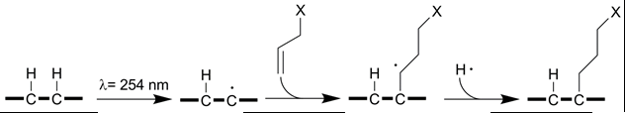
\includegraphics[width=\linewidth]{Abbildungen/OF_Funktionalisierung.png}
		} % scalebox
		\subcaption{}
		\label{subfig:Hauptreaktion}
	\end{subfigure}

	\begin{subfigure}[h]{\textwidth}
		\centering
		\scalebox{\hscaleOne}{
			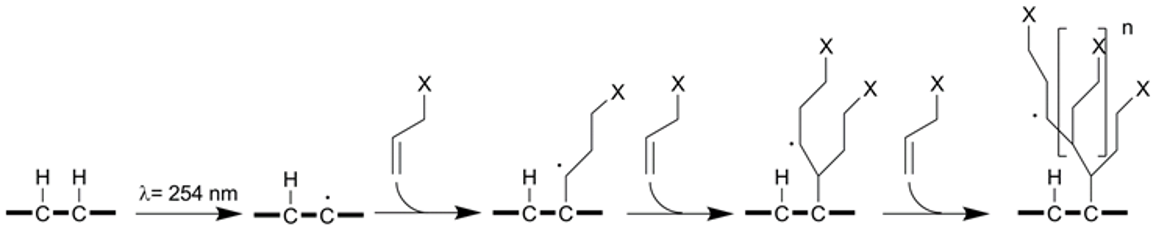
\includegraphics[width=\linewidth]{Abbildungen/OF_Funktionalisierung_Nebenreaktionen_a.png}
		} % scalebox
		\subcaption{}
		\label{subfig:Nebenreaktion-a}
	\end{subfigure}

	\begin{subfigure}[h]{\textwidth}
		\centering
		\scalebox{\hscaleOne}{
			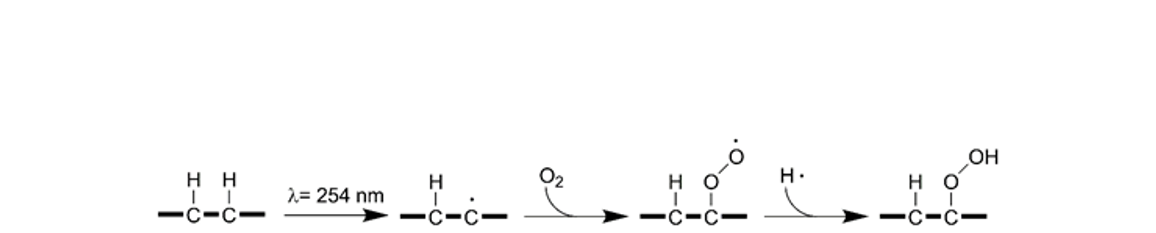
\includegraphics[width=\linewidth]{Abbildungen/OF_Funktionalisierung_Nebenreaktionen_b.png}
		} % scalebox
		\subcaption{}
		\label{subfig:Nebenreaktion-b}
	\end{subfigure}

	\begin{subfigure}[h]{\textwidth}
		\centering
		\scalebox{\hscaleOne}{
			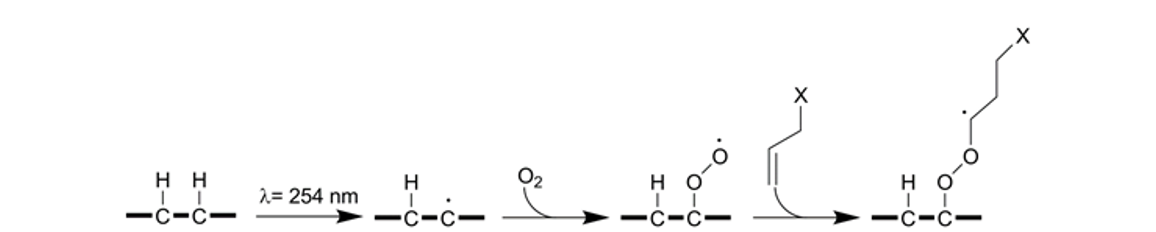
\includegraphics[width=\linewidth]{Abbildungen/OF_Funktionalisierung_Nebenreaktionen_c.png}
		} % scalebox
		\subcaption{}
		\label{subfig:Nebenreaktion-c}
	\end{subfigure}
	
	\caption{Reaktion der Oberflächenfunktionalisierung. a) Start der radikalischen Reaktion ist die Bestrahlung der Kohlenstoffoberfläche des Substrats und der \spitze~durch UV-Licht der Wellenlänge $\lambda~=~254~nm$. Im Verlauf der Reaktion wird ein Allylamin-Molekül ($X~=~NH_2$) an die Oberflächen von \spitze~und Substrat angelagert. Das ungepaarte Elektron am Kohlenstoffrückgrat des Allylamin wird über ein Wasserstoffradikal abgesättigt. Während der Funktionalisierung sind folgende Nebenreaktionen möglich: b). Baumartiges Wachstum von Allylamin-Molekülen, bedingt durch eine zu hohe Allyaminkonzentration. b) Terminierung des Substrats/ \spitze~mit \carboxys~durch den Einbau von molekularem Sauerstoff. c) Bildung von Peroxid artigen Strukturen zwischen Substrat/ \spitze~und Allylamin, bedingt durch den Einbau von molekularem Sauerstoff.}
	
	\label{fig:OF_Funktionalisierung}
\end{figure}

\subsection{Kopplung der Spacermoleküle an funktionalisierte Oberflächen}
\label{subsec:kopplung_der_spacermoleküle_an_funktionalisierte_oberfläche}

Die Bildung der \amid~erfolgt durch eine  Standard Kopplungschemie über \ac{EDC} und \ac{NHS} \cite{Hermanson.2013,MichaelF.Pill.2015}. Als Spacermolekül wurde \ac{CMA} verwendet. \abb~\ref{fig:Kopplungschemie} zeigt die Kopplung von \spacer~und Substrat bzw. \spitze. $R_1$ stellt den \spacer~dar, dessen \carboxys~zunächst durch \ac{EDC} aktiviert und anschließend durch \ac{NHS} in \ester~überführt werden. Die Bildung der \amid~erfolgt schließlich zwischen den \estern~und den \aminos~des funktionalisierten Substrats bzw. \spitze~($R_2$). Wie aus \abb~ \ref{fig:Kopplungschemie} zu erkennen ist, wird \ac{NHS} durch die Reaktion mit einem primären Amin im Kreislauf gehalten. \ac{EDC} hingegen reagiert während der Aktivierung der \carboxys~zu einem nicht reaktiven Isourea ab.

\begin{figure}[H]
	\begin{flushleft}
		\scalebox{\hscaleOne}{\begin{minipage}{\textwidth}
				\schemedebug{false}
				\schemestart
				\chemname{\Rest}{Carbonsäure} 
				\arrow(.south--.north west){-U>[*{0.south west}\chemname{\EDC}{EDC}][][][.5][]}[-90,4] 
				\chemname{\OAcylisourea}{O-Acylisourea Zwischenprodukt}
				\arrow{-U>[*{0.south}\chemname{\NHS}{NHS}][][][.5][]}[,3]
				\chemname{\Ester}{NHS Ester Zwischenprodukt}
				\arrow{-U>[*{0.north east}\chemname{\PrimAmin}{Primäres Amin}][*{0.east}\chemname{\NHS}{NHS}][][.3][60]}[90,4]
				\chemname{\Amidbindung}{Bildung der Amidbindung}
				\schemestop
			\end{minipage}
		}
	\end{flushleft}
	\caption[Reaktionsschema der Kopplungschemie über \acs*{EDC} und \acs*{NHS}]{Reaktionsschema der Kopplungschemie über \acs*{EDC} und \acs*{NHS}: Beginn der Kopplung ist die Aktivierung eines Moleküls mit Carboxylgruppe ($R_1-COOH$) mittels \acs*{EDC}. Das dabei entstandene Isourea Zwischenprodukt wird in einem zweiten Schritt über Zufuhr von \acs*{NHS} das aktivierte \ester~Zwischenprodukt gebildet. Zuletzt wird über den Angriff eines Nucleophils ($R_2-NH_2$) die Amidbindung gebildet.}
	\label{fig:Kopplungschemie}
\end{figure}

\section{Hydrolyse der Amidbindung}
\label{sec:hydrolyse_der_amidbindung}

Die Hydrolyse ist eine spezielle Art der Solvolyse, die Auflösung einer chemischen Bindung unter Beteiligung von Lösungsmittelmolekülen. Sie verläuft nach dem $S_N2$-Mechanismus pseudo-erster Ordnung, da die Konzentration des Lösungsmittel annähernd konstant bliebt \cite[91]{Hadener.2006}. Alternativ kann die Hydrolyse der \amid~auch als eine Reaktionskaskade einer Additionsreaktion, gefolgt von einer Eliminierungsreaktion angesehen werden \cite[288]{Latscha.2016}. Unter neutralen Bedingungen verläuft die Amidhydrolyse nach dem Schema, dargestellt in \abb~\ref{fig:amid_neutral} ab \cites[288]{Latscha.2016}{Zahn.2004b}.\\

Zunächst bindet ein Wassermolekül mit einem freien Elektronenpaar am Carbonylkohlenstoff von N1. Dabei dissoziiert das addierte Wasser und ein Proton wird direkt, über einen Grotthuß-artigen Mechanismus auf den Stickstoff des \ac{TZP} N2 übertragen. Anschließend lagern sich die Elektronen in N2 um und regenerieren im zweiten Schritt die \carboxys~am \spacer~($R_1-COOH$) N3 und die \amino~auf dem Substrat bzw. der \spitze~($R_2-NH_2$) N4.

\begin{figure}[H]
	\begin{flushleft}
		\scalebox{\hsclaeChemfig}{\begin{minipage}{\textwidth}
				\setchemfig{scheme debug = false}
				\schemestart
				\Wasser
				\hspace{1cm}
				\chemname{\Amidbindung}{N1}
				\chemmove[shorten <= 5pt, shorten >= 2pt]{\draw[dashed](n1)..controls +(north east:1.5cm) and +(south:2.75cm)..(n2);}
				\arrow{<=>}
				\chemname{\AmidbindungII}{N2}
				\chemmove[shorten <= 5pt, shorten >= 2pt]{\draw[dashed](n4)..controls +(east:0.5cm) and +(east:0.75cm)..(n3);
					\draw[dashed](n5)..controls +(north east:0.5cm) and +(north:0.5cm)..(n6);}
				\arrow{<=>}
				\chemname{\Acid}{N3} \+ \chemname{\PrimAmin}{N4}
				\schemestop
			\end{minipage}
		}
	\end{flushleft}
	\caption[Hydrolyse der Amidbindung im neutralen Milieu]{Hydrolyse der Amidbindung im neutralen Milieu. Der Angriff des Wassers erfolgt am Carbonylkohlenstoff von N1. Dabei dissoziiert das Wassermolekül und ein Proton wird über einen Grotthuß artigen Mechanismus auf das Stickstoffatom von N2 übertragen. Nach einer Reihe interner Elektronenumlagerungen bricht im zweiten Schritt die Amidbindung unter Rückbildung der \spacer~($R_1-COOH$) N3 und des Substrats ($R_2-NH_2$) N4.}
	
	\label{fig:amid_neutral}
\end{figure}

\subsection{Sauer katalysierte Amidhydrolyse}
\label{subsec:sauer_katalysierte_amidhydrolyse}

Die saure Katalyse der Amidhydrolyse beruht auf der erhöhten Polarität der \carboxy~durch Addition eines Protons an das Carbonylsauerstoff. Die Reaktion läuft dabei nach dem Schema, dargestellt in \abb~\ref{fig:amid_sauer} ab \cites[288]{Latscha.2016}{Zahn.2004b}{Zahn.2003}\\

Nach der Bildung des Carbeniumions (S1) erfolgt der nucleophile Angriff des Wassers. Dieses dissoziiert dabei in ein \ch{OH-}-Ion und ein \ch{H+}-Ion. Während das \ch{OH-}-Ion an den positiv geladenen Carbonylkohlenstoff addiert wird, geht das gebildete \ch{H+}-Ion in Lösung. Im zweiten Schritt wird das \ac{TZP} (S2) durch ein weiteres \ch{H+}-Ion aus der Lösung am Stickstoffatom protoniert und S3 gebildet. Im letzten Schritt wird die \amid~durch eine Reihe interner Elektronenumlagerungen gebrochen. Dabei werden die \carboxys~des \spacer~($R_1-COOH$) S4 und \aminos~des Substrats bzw. der \spitze~($R_2-NH_3^+$) S5 regeneriert.\\

Die Reaktionsmechanismen der Amidhydrolyse im Sauren, sowie im Neutralen sind sich sehr ähnlich. Der Unterschied besteht in der Art und Weise wie das Stickstoffatom protoniert wird, dies zeigt eine theoretische Studie von D.~Zahn~\textit{et al}.~\cites{Zahn.2004b}.

\begin{figure}[H]
	\begin{flushleft}
		\scalebox{\hsclaeChemfig}{\begin{minipage}{\textwidth}
				\setchemfig{scheme debug = false}
				\schemestart
				\Wasser
				\hspace{0.1cm}
				\chemname{\AmidbindungIII}{S1}
				\chemmove[shorten <= 5pt, shorten >= 5pt]{\draw[dashed](n1)..controls +(north east:1.5cm) and +(240:2.75cm)..(pa1);}
				\arrow{<=>[-H$_{\mathrm{aq}}^{\tiny +}$][+H$_{\mathrm{aq}}^{\tiny +}$]}
				\chemname{\AmidbindungIV}{S2}
				\arrow{<=>[+H$_{\mathrm{aq}}^{\tiny +}$][-H$_{\mathrm{aq}}^{\tiny +}$]}
				\chemname{\AmidbindungV}{S3}
				\chemmove[shorten <= 2pt, shorten >= 2pt]{\draw[dashed](av2)..controls +(north:1.5cm) and +(west:1.5cm)..(av1);
					\draw[dashed](av4)..controls +(350:0.75cm) and +(south east:0.75cm)..(av3);}
				\arrow{<=>}
				\chemname{\Acid}{S4} \+ \chemname{\PrimAminII}{S5}
				\schemestop
			\end{minipage}
		}
	\end{flushleft}
	\caption[Reaktionsmechanismus der sauer katalysierten Amidhydrolyse]{Reaktionsmechanismus der sauer katalysierten Amidhydrolyse. Das durch die Protonierung des Carbonylsauerstoff entstandene Carbeniumion S1 ist sehr viel reaktiver als die unveränderte Carbonylgruppe. Der nucleophile Angriff kann daher sehr viel schneller erfolgen als vor der Protonierung. Während des nucleophilen Angriffs dissoziiert das Wassermolekül, das gebildete \ch{H+}-Ion geht in Lösung, das \ch{OH-}-Ion wird an das Carbonylkohlenstoff addiert und bildet das tetraedrische Zwischenprodukt S2. In einem dritten Schritt wird durch ein weiteres \ch{H+}-Ion das Stickstoffatom protoniert, wodurch das Zwischenprodukt S3 gebildet wird. Nach einer Reihe interner Elektronenumlagerungen bricht die Amidbindung unter Rückbildung des \spacers~($R_1-COOH$) S4 und des Substrat/ \spitze~($R_2-NH_3^+$) S5.}
	
	\label{fig:amid_sauer}
\end{figure}

\subsection{Basisch katalysierte Amidhydrolyse}
\label{subsec:basisch_katalysierte_amidhydrolyse}

Während der basischen Katalyse der Amidhydrolyse wird in einer vorgelagerten Gleichgewichtsreaktion aus dem weniger nucleophilen Wasser das sehr viel nucleophilere \ch{OH-}-Ion gebildet. Danach läuft die Reaktion nach dem Schema in \abb~\ref{fig:amid_basisch} ab \cites[288]{Latscha.2016}{Zahn.2004b}{Zahn.2004}\\

Das gebildete \ch{OH-}-Ion greift den Carbonylkohlenstoff der Amidbindung B1 an und es wird das \ac{TZP} B2 gebildet. Nachdem ein solvatisiertes \ch{H+}-Ion aus der Lösung in die Nähe von B2 diffundiert ist, wird das Stickstoffatom in B2 protoniert und es bildet sich das \ac{ZI} B3. Anschließend erfolgt nach einer Reihe interner Elektronenumlagerungen im letzten Schritt der Bruch der Amidbindung und es wird die \carboxy~am \spacer~($R_2-COOH$, B4), sowie die \amino~auf dem Substrat regeneriert.\\

Mit steigendem pH-Wert ist es außerdem möglich, dass die verbleibenden \carboxy~am \ac{ZI} (B3) zusätzlich deprotoniert wird \cites{Zahn.2004}. Dadurch entsteht statt der Carbonsäure in B4 das Carboxylation.

\begin{figure}[H]
	\begin{flushleft}
		\scalebox{\hsclaeChemfig}{\begin{minipage}{\textwidth}
			\setchemfig{scheme debug = false}
			\schemestart
				\OHIon
				\hspace{0.5cm}
				\chemname{\Amidbindung}{B1}
				\chemmove[shorten <= 5pt, shorten >= 2pt]{\draw[dashed](oh)..controls +(330: 1cm) and +(260:1cm)..(n2);
				}
				\arrow{<=>}
				\chemname{\AmidbindungVI}{B2}
				\arrow{<=>[+H$_{\mathrm{aq}}^{\tiny +}$][-H$_{\mathrm{aq}}^{\tiny +}$]}
				\chemname{\AmidbindungVII}{B3}
				\chemmove[shorten <= 5pt, shorten >= 2pt]{\draw[dashed](aoh2)..controls +(east:0.5cm) and +(east:0.75cm)..(aoh1);
					\draw[dashed](aoh3)..controls +(north east:0.5cm) and +(north:0.5cm)..(aoh4);
				}
				\arrow{<=>}
				\chemname{\Acid}{B4} \+ \chemname{\PrimAmin}{B5}
			\schemestop
		\end{minipage}
	}
	\end{flushleft}
	\caption[Reaktionsmechanismus der basisch katalysierten Amidhydrolyse]{Reaktionsmechanismus der basisch katalysierten Amidhydrolyse. Durch eine vorgelagerte Gleichgewichtsreaktion entsteht aus Wasser ein nucleophileres \ch{OH-}-Ion. Dieses greift statt Wasser am Carbonylkohlenstoff der Amidbindung von B1 an und bildet das tetraedrische Zwischenprodukt B2. Im zweiten Schritt diffundiert ein \ch{H+}-Ion aus der Lösung und protoniert das Stickstoffatom in B2. Dabei wird das zwitterionische Zwischenprodukt B3 gebildet. Nach einer Reihe interner Elektronenumlagerungen bricht die Amidbindung unter Rückbildung des \spacers~($R_1-COOH$) B4 und des \substrats/ \spitze~($R_2-NH_2$) B5.}
	
	\label{fig:amid_basisch}
\end{figure}

\subsection{Energieprofil der Amidhydrolyse ohne Krafteinfluss}
\label{subsec:energieprofil_der_amidhydrolyse_ohne_krafteinfluss}
Energetisch gesehen durchläuft die Hydrolyse der \amid~zwei prominenten Barrieren, wie in \abb~\ref{fig:energieprofil_ohne_kraft} dargestellt \cite{Zahn.2003,Zahn.2004,Zahn.2004b}. Um den \ac{UZ}1 - die innere Barriere - zu überwinden wird eine Aktivierungsenergie von ca. $147~kJ~mol^{-1}$ im neutralen Milieu~\cites{Zahn.2004b}, $78~kJ~mol^{-1}$ im sauren Milieu~\cites{Zahn.2003} und ca. $66~kJ~mol^{-1}$ im basischen Milieu~\cites{Zahn.2004} benötigt. Für den \ac{UZ}2 - die äußere Barriere - weitere $38~kJ~mol^{-1}$ im sauren Milieu~\cites{Zahn.2003} und $72~kJ~mol^{-1}$ im basischen Milieu\cites{Zahn.2004}. Es sind keine Angaben für \ac{UZ}2 im neutralen Milieu verfügbar. Der Übergang von \ac{TZP} zum \ac{ZI} wird als barrierefrei angesehen. Für die Rückreaktion des \ac{TZP} zum Eduktzustand im sauren/ basischen Milieu ist lediglich eine Aktivierungsenergie von $12-20~kJ~mol^{-1}$ notwendig~\cite{Zahn.2004,Zahn.2003}. Aufgrund dieser Tatsache ist die Rückreaktion vom \ac{TZP} bzw. \ac{ZI} zum Eduktzustand wahrscheinlicher, als die Vorwärtsreaktion zum Produktzustand und erklärt die lange Lebensdauer der \amid~von mehreren Dekaden bis hin zu mehreren Jahrhunderten \cite{Radzicka.,Berg.2018}.

\begin{figure}[h]
	\centering
	\scalebox{\hscaleOne}{
		\includegraphics[width=\linewidth]{Abbildungen/Energieprofil_ohne_Kraft.png}
	} % scalebox
	\caption[Energieprofil der Amidhydrolyse ohne Einfluss einer äußeren Kraft]{Energieprofil der Amidhydrolyse ohne Einfluss einer äußeren Kraft. Die Höhe der inneren Barriere \acs*{UZ}1 liegt bei $147~kJ~mol^-1$~\cite{Zahn.2004b} (neutral), $78~kJ~mol^{-1}$\cite{Zahn.2003} (sauer katalysiert) und $66~kJ~mol^{-1}$~\cite{Zahn.2004} (basisch katalysiert). Die Höhe der äußeren Barriere \acs*{UZ}2 liegt bei $38~kJ~mol^{-1}$~\cite{Zahn.2003} (sauer katalysiert) und $72~kJ~mol^{-1}$~\cite{Zahn.2004} (basisch katalysiert). Für den Bruch der Amidbindung im neutralen Milieu liegen keine Daten vor. Die Überführung des \acs*{TZP} in \acs*{ZI} läuft annähernd barrierefrei.}
	\label{fig:energieprofil_ohne_kraft}
\end{figure}

\subsection{Bindungskinetik unter Krafteinfluss}
\label{subsec:bindungskinetik_unter_krafteinfluss}

Ein bekanntes Modell, um die Kraftabhängigkeit chemischer Bindungen zu beschreiben, stammt von Zhurkov und Bell \cite{Zhurkov.1984,Bell.1978}:

\begin{equation}
	E_a(F)~=~\Delta E_{a,0}~-~F \cdot \Delta x^\ddag
	\label{eq:bell_modell}
\end{equation}

Dabei steht $\Delta E_{a,0}$ für die Aktivierungsenergie des Bindungsbruchs ohne Krafteinfluss (hier die Höhe von \ac{UZ}2), $\Delta x^{ddag}$ für den Abstand von einem Produktzustand zu einem Übergangszustand entlang der Reaktionskoordinate (hier von \ac{ZI} zu \ac{UZ}2).\\

In \abb~\ref{fig:energieprofil_mit_kraft} sind exemplarisch die Energieprofile der basisch katalysierten Amidhydrolyse bei verschiedenen Kräften, berechnet nach dem Modell von Zhurkov und Bell, dargestellt. Ab einer Kraft von $500~pN$ (\abb~\ref{fig:energieprofil_mit_kraft}, blauer Graph) liegen \ac{UZ}1 und \ac{UZ}2 in etwa bei derselben Aktivierungsenergie ($64~kJ~mol^{-1}$ bzw. $68~kJ~mol^{-1}$) und \ac{UZ}1 beginnt die Kinetik der Reaktion zu bestimmen. Bei einer Kraft von $800~pN$ (\abb~\ref{fig:energieprofil_mit_kraft}, roter Graph) liegt \ac{UZ}2 ($49~kJ~mol^{-1}$) deutlich unterhalb von \ac{UZ}1 ($63~kJ~mol^{-1}$) und \ac{UZ}1 dominiert die Kinetik der Reaktion vollständig.\\

% Energieprofil mit Kraft
\begin{figure}[h]
	\centering
	\scalebox{\hscaleOne}{
		\includegraphics[width=\linewidth]{Abbildungen/Energieprofil_mit_Kraft.png}
	} % scalebox
	\caption[Energieprofil der Amidhydrolyse unter dem Einfluss einer äußeren Kraft]{Energieprofil der Amidhydrolyse unter dem Einfluss einer äußeren Kraft am Beispiel der basisch katalysierten Hydrolyse. Die Energien einzelner \acs*{UZ} und \acs*{ZI} wurden über das Modell von Zhurkov und Bell berechnet. Für eine Zugkraft von 500 pN (blau) rückt \acs*{UZ}2 (ca. $68~kJ~mol^{-1}$) in den Bereich von \acs*{UZ}1 (ca. $64~kJ~mol^{-1}$). Bei einer Zugkraft von 800 pN (rot) liegt \acs*{UZ}2 (ca. $49~kJ~mol^{-1}$) unterhalb von \acs*{UZ}1 (ca. $49~kJ~mol^{-1}$).}
	\label{fig:energieprofil_mit_kraft}
\end{figure}


Zusammen mit \gl~\ref{eq:bell_modell} und der Arrhenius-Gleichung erhält man die kraftabhängige Geschwindigkeitskonstante $k(F)$ für den Bruch einer chemischen Bindung\footnote{Unter Krafteinwirkung entlang der Bindungsachse} \cite{RibasArino.2012}:

\begin{equation}
	k(F)~=~k_0 \cdot e^{\frac{F \cdot \Delta x^\ddag}{k_B T}}
	\label{eq:k_kraftabhängig}
\end{equation}

Mit $k_B$ der Boltzmannkonstante, $k_0$ der Geschwindigkeitskonstante des Bindungsbruchs ohne äußere Kraft und $T$ der absoluten Temperatur in Kelvin. Der allgemeine Zusammenhang zwischen Geschwindigkeitskonstante und der Zeitkonstante eines Prozesses lautet:

\[ k~=~\frac{1}{\tau} \]

Damit ergibt sich der Ausdruck für die Kraftabhängige, mittlere Lebensdauer \cite{Glockner.2011}:

\begin{equation}
	\tau(F)~=~\tau_0 \cdot e^{- \frac{F \cdot \Delta x^\ddag}{k_BT}}
	\label{eq:tau_kraftabhängig}
\end{equation}

Wobei $\tau_0$ die mittlere Lebensdauer einer chemischen Bindung ohne äußre Kraft bezeichnet. Wird eine Kraft entlang der C-N-Bindung eines Amids angelegt, so wird die äußere Barriere effektiver abgesenkt, als die innere Barriere \cite{Xia.2011,Tian.2013}. Dieses Verhalten wird damit begründet, dass die Reaktionskoordinate für die innere Barriere\footnote{Meist der Abstand zwischen dem Sauerstoffatom eines angreifenden \ch{H20}-Moleküls bzw. \ch{OH-}-Ions und dem Carbonylkohlenstoff.} nahezu senkrecht zur Kraftrichtung läuft. Die Reaktionskoordinate für die äußere Barriere\footnote{Meist der Abstand des Carbonylkohlenstoff und dem Stickstoffatom des Amids.} hingegen liegt parallel zur äußeren Kraft. Die beiden Reaktionskoordinaten sind voneinander unabhängig. Auf Force-Clamp-Experimente übertragen bedeutet das, dass die Änderung des C-N-Abstandes nicht die Geschwindigkeit beeinflusst, mit der ein Nucleophil die Carbonylgruppe angreift (vgl.~Abschnitt~\ref{sec:hydrolyse_der_amidbindung}).\\

In dieser Arbeit ist die Zeit, bei der eine spezifische Bindung bricht, der experimentell zugängliche Parameter. Sinnvoll ist daher die quantitative Bestimmung von $k$ durch die Betrachtung des Reaktion von  \ac{ZI} zum Produktzustand als eine Reaktion 1. Ordnung \cite{MichaelF.Pill.2015}:

\begin{equation}
	N(t)~=~N_0 \cdot e^{-k \cdot t}
	\label{eq:exponentieller_zerfall}
\end{equation}

$N(t)$ steht für die Anzahl der zum Zeitpunkt $t$ intakten \amide~und $N_0$ für die Anzahl aller gemessenen \amide. Durch den Fit dieses exponentiellen Zerfalls an die Messdaten kann $k$ als freier Parameter bestimmt werden.\\
In manchen Fällen kommt es vor, dass in den gemessenen Daten zwei Zerfallsprozesse auftreten. Für solche Fälle lässt \gl~\ref{eq:exponentieller_zerfall} zu einem biexponentiellen Zerfall erweitern:

\begin{equation}
	N(t)~=~N_0 \cdot [A \cdot e^{-k_1 \cdot t}~+~(A~-~1) \cdot e^{-k_2 \cdot t}]
	\label{eq:biexponentieller_zerfall}
\end{equation}

Hierbei stehen die beiden Geschwindigkeitskonstanten $k_1$ und $k_2$ für einen schnellen, bzw. für einen langsamen Prozess. Der Mischungskoeffizient $A$ ist definiert als:

\[ A~=~\frac{N_{0,1}}{N_0} \]

Und

\[ (1~-~A)~=\frac{N_0~-~N_{0,1}}{N_0}~=~\frac{N_{0,2}}{N_0} \]

Wobei $N_{0,1}$ für die Anzahl aller Spezies mit $k_1$ bzw. $N_{0,2}$ für die Anzahl aller Spezies mit $k_2$ und $N_0~=~N_{0,1}~+~N_{0,2}$ für die Anzahl aller gemessen Bindungen.

\section{Rasterkraftmikroskop}
\label{sec:rasterkraftmikroskop}

Das Rasterkraftmikroskop (\ac{AFM}) wurde ursprünglich von Binnig, Quate und Gerber im Jahr 1986 entwickelt \cite{Binnig.1986}. Es diente als Weiterentwicklung des Rastertunnelmikroskops zur Abbildung von Oberflächen nichtleitender Proben. Den heutigen Aufbau des \acp{AFM} und eine Übersicht über einige Anwendungen gibt z.B. McConney \textit{et al}. \cite{McConney.2010}. Eine schematische Darstellung des \acp{AFM} zeigt \abb~\ref{fig:afm_schema}. Das Herzstück des \acp{AFM} ist eine \spitze~am Ende eines Cantilevers, auf dessen Rückseite ein Laserstrahl ausgerichtet wird (\abb~\ref{fig:afm_schema}a). Die Reflektion des Laserstrahls wird von einer segmentierten Photodiode erfasst (\abb~\ref{fig:afm_schema}b). Wird die Oberfläche mit der sehr feinen Messspitze\footnote{Im Idealfall sitzt ein einzelnes Atom am Ende der Spitze.}  (\abb~\ref{fig:afm_schema}c)) über die x-, y- und z- Piezos (\abb~\ref{fig:afm_schema}d)) abgerastert, führen Wechselwirkungen von \spitze~und Substrat zu einer Auslenkung des Cantilevers. Diese Auslenkung wird durch die segmentierte Photodiode gemessen.\\

\begin{figure}[h]
	\centering
	\scalebox{\hscaleOne}{
		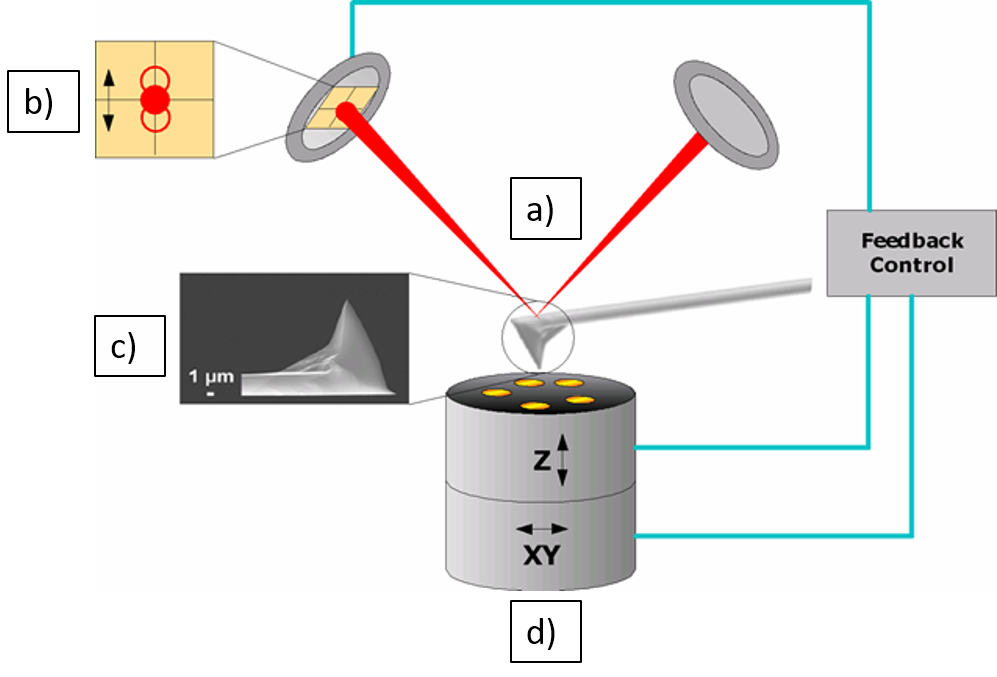
\includegraphics[width=\linewidth]{Abbildungen/AFM.png}
	} % scalebox
	\caption[Schematische Darstellung des Rasterkraftmikroskops]{Schematische Darstellung des Rasterkraftmikroskops. Die wichtigsten Komponenten sind: a) Cantilever mit ausgerichtetem Laserstrahl. b) Segmentierte Photodiode. c) Die Messspitze am Ende des Cantilever. d) x-, y- und z-Piezos.}
	\label{fig:afm_schema}
\end{figure}

Für die durchgeführten einzelmolekülspektroskopischen Untersuchungen (\ac{SMFS}), wird zwischen \spitze~und Substrat, mittels der in Abschnitt~\ref{subsec:kopplung_der_spacermoleküle_an_funktionalisierte_oberfläche} beschriebenen Chemie, ein \spacer~gebunden. Beim Zurückziehen des z-Piezos wird das Molekül gestreckt und der Cantilever ausgelenkt.\\

\ac{SMFS}-Experimente werden anhand der Kraftdynamik am \space~ charakterisiert. Wird die wirkende Kraft zeitlich konstant gehalten, wird von Force-Clamp-\ac{SMFS} gesprochen.\\
In Force-Clamp-Experimenten wird der \spacer~bis zu einer Kraft gestreckt, bei der noch kein Bindungsbruch stattfindet. Dabei wird die Zeit gemessen, bis die Bindung durch thermisch aktivierte Prozesse bricht.\\

Wirkt die Kraft am \spacer~zeitlich nicht konstant, wird von Force-Ramp-Experimenten gesprochen.\\
In Force-Ramp-Experimenten wird das Spacermolekül mit konstanter Geschwindigkeit in z-Richtung gestreckt. Der z-Piezo wird dabei bis zum Bindungsbruch des \spacer~an den Kopplungspunkten (\spitze~oder Substrat) zurückgezogen.

\section{Einzelmolekülspektroskopie am Rasterkraftmikroskop}
\label{sec:einzelmolekülspektroskopie_am_rasterkraftmikroskop}

\subsection{Molekularer Aufbau des Versuchssystems}
\label{subsec:molekularer_aufbau_des_Versuchssystems}

Der Fokus dieser Arbeit liegt auf der Untersuchung der \amid~ (Rot dargestellte Atomgruppe in \abb~\ref{fig:molekularer_aufbau}). Durch die verwendete Kopplungschemie (vgl. Reaktionsschema aus \abb~\ref{fig:Kopplungschemie}) bildet sich die \amid~zwischen den primären \aminos~von Substrat bzw. \spitze~und den \carboxys~von \ac{CMA}. Die Anzahl an \ac{CMA}-Monomeren zischen den \amide~ist beliebig. Der vollständige molekulare Aufbau des Versuchssystems, wie in \abb~\ref{fig:molekularer_aufbau} dargestellt, zeigt exemplarisch die Verbindung von Substrat und \spitze.

\begin{figure}[h]
	\centering
	\scalebox{\hscaleZero}{
		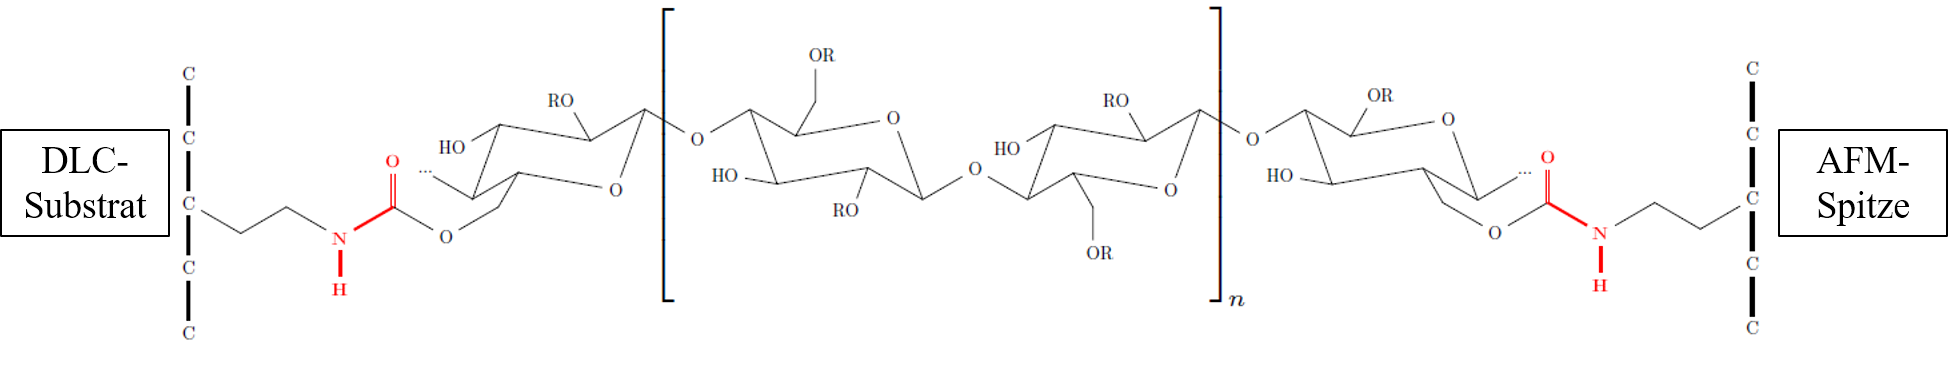
\includegraphics[width=\linewidth]{Abbildungen/molekularer_aufbau.png}
	} % scalebox
	\caption[Molekularer Aufbau der \acs*{SMFS}-Experimente]{Molekularer Aufbau der \acs*{SMFS}-Experimente. In rot sind die untersuchten Amidbindungen zwischen Allylamin und \acs*{CMA} dargestellt.}
	\label{fig:molekularer_aufbau}
\end{figure}

\subsection{Kraftkurven}
\label{subsec:kraftkurven}

In \ac{SMFS}-Experimenten kann die Kraft als Funktion des Wegs (Kraft-Abstand-Kurven), oder als Funktion der Zeit (Kraft-Zeit-Kurven) dargestellt werden. In der Kraft-Abstand-Darstellung lassen sich \ac{CMA}-Spezifische Einzelmolekülinteraktionen identifizieren und in der Kraft-Zeit-Darstellung lässt sich die Clampzeit ermitteln. Um kleinere Abrisse oder Sprünge in der Kraft besser zu erkennen, bietet sich die Weg-Zeit Darstellung der Kraftkurven an. Anhand dieser Darstellungsart lässt sich aus dem Graphen die Geschwindigkeit des z-Piezos ermitteln. Die Steigung ist im Betrag umso größer, je höher die Geschwindigkeit des Piezos war. Bei Abrissen steht der Graph annähernd senkrecht zur Zeit-Achse. \\

Es wurden an einer Probe Force-Ramp-, sowie Force-Clamp-Experimente durchgeführt. Letztere dienen ausschließlich des Zwecks zu überprüfen, ob \ac{CMA}-Spezifische Einzelmolekülinteraktionen auftraten. Force-Clamp-Experimente hingegen werden genutzt, um Abrisszeiten und somit die Geschwindigkeitskonstante der Experimente zu bestimmen.\\

Eine typische Kraftkurve der Force-Ramp-Experimente zeigt \abb~\ref{fig:force_ramp_kurve}. Diese Kurven sind insgesamt in drei Segmente untergliedert:

\begin{enumerate}
	\renewcommand\labelenumi{\bfseries\theenumi.}
	
	\item Hinfahrkurve (\abb~\ref{fig:force_ramp_kurve}, blau)
	\item Ruhezeit (\abb~\ref{fig:force_ramp_kurve}, Orange)
	\item Rückfahrkurve (\abb~\ref{fig:force_ramp_kurve}, Gelb)
	
\end{enumerate}

Im 1. Segment wird die \spitze~mit einer bestimmten Geschwindigkeit (hier $6~µm~s^{-1}$) an das Substrat angenähert, bis eine vorgegebene Auslenkung des Cantilevers (hier $250~pN$) erreicht ist. Um der Ausbildung von \amid~genügend Zeit zu geben, ruht die \spitze~im 2. Segment für ca. 3 Sekunden bei konstanter Kraft auf dem Substrat. Im 3. Segment wird die \spitze~mit einer bestimmten Geschwindigkeit (hier $6~µm~s^{-1}$) wieder von der Substratoberfläche entfernt. Dabei wird der \spacer~bis zum Bruch der \amid~zwischen \spacer~und Substrat bzw. \spitze~gestreckt. Eine vollständige Zusammenstellung der Parameter für ein Force-Clamp-Experiment enthält Tabelle~\ref{tab:force-ramp-parameter} in Abschnitt~\ref{subsec:durchführung_von_clamp/_ramp_versuchen}.\\

\begin{figure}[h]
	\centering
	\scalebox{\hscaleZero}{
		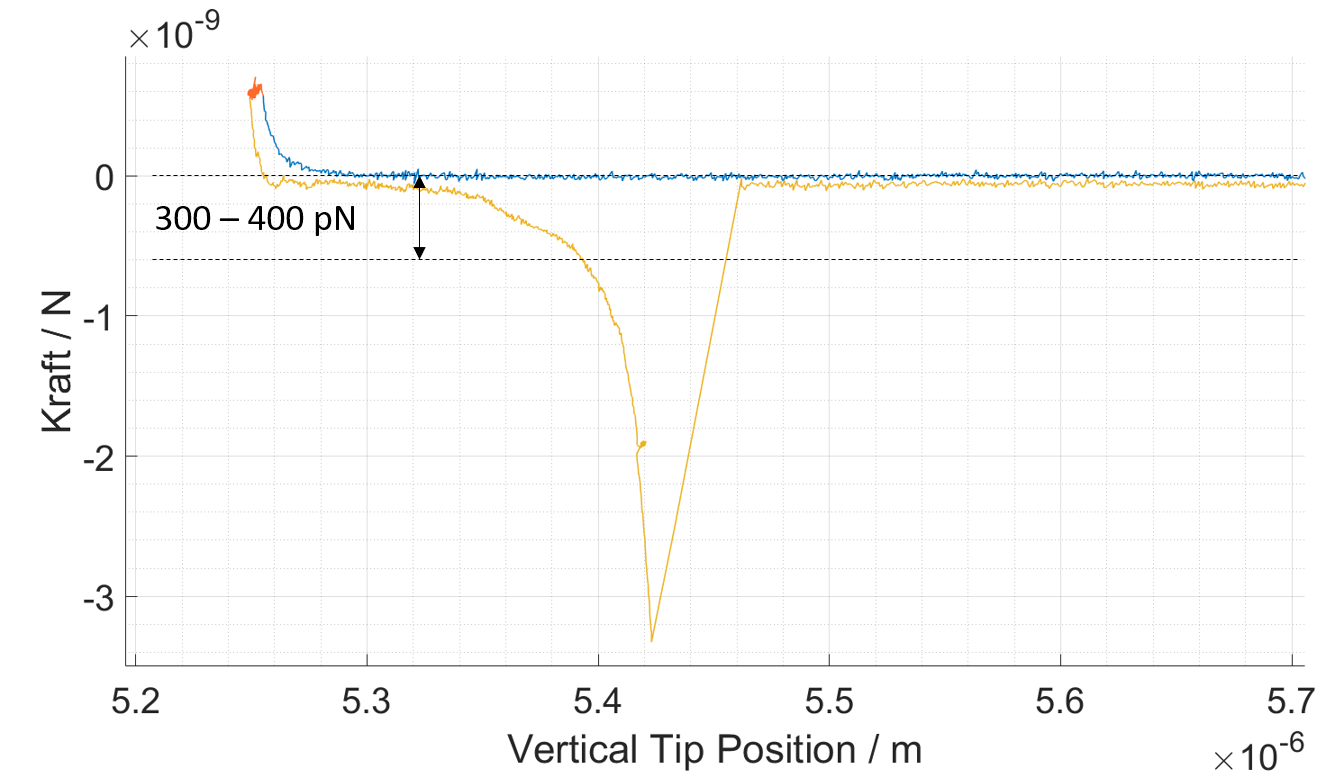
\includegraphics[width=\linewidth]{Abbildungen/Bsp_Force_Ramp_III.png}
	} % scalebox
	\caption[Beispiel einer Force-Ramp-Kraftkurve]{Beispiel einer Force-Ramp-Kraftkurve (Kraft-Abstand-Kurve). Blau: Hinfahrkurve. Orange: Ruhezeit. Gelb: Wegfahrkurve. Hervorgehoben ist das \acs*{CMA}-Spezifische Plateau bei 300 - 400 pN.}
	\label{fig:force_ramp_kurve}
\end{figure}

Typische Ergebnisse aus Force-Clamp-Experimenten zeigt \abb~\ref{fig:force_clamp_kurve}. Dabei zeigt \abb~\ref{subfig:kraft_abstand} die Kraft-Abstand Form und \abb~\ref{subfig:kraft_zeit} die Kraft-Zeit Form dieser Kraftkurve. Insgesamt sind Force-Clamp-Experimente in sechs Segmente untergliedert:

\begin{enumerate}
	\renewcommand\labelenumi{\bfseries\theenumi.}
	
	\item Hinfahrkurve (\abb~\ref{subfig:kraft_abstand} und \abb~\ref{subfig:kraft_zeit}, blau)
	\item Ruhezeit (\abb~\ref{subfig:kraft_abstand} und \abb~\ref{subfig:kraft_zeit}, orange)
	\item Initial Retract (\abb~\ref{subfig:kraft_abstand} und \abb~\ref{subfig:kraft_zeit}, gelb)
	\item Clamp Retract (\abb~\ref{subfig:kraft_abstand} und \abb~\ref{subfig:kraft_zeit}, lila)
	\item Clamp (\abb~\ref{subfig:kraft_abstand} und \abb~\ref{subfig:kraft_zeit}, grün)
	\item Retract (\abb~\ref{subfig:kraft_abstand} und \abb~\ref{subfig:kraft_zeit}, schwarz)
	
\end{enumerate}

Die Kraft-Abstand-Kurven wurden zur Evaluierung der Einzelmolekülinteraktion und zur Kategorisierung (s.~Abschnitt~\ref{subsec:kategorisierung_der_kraftkurven}) genutzt. Die Kraft-Zeit-Kurven dienen der Bestimmung der Clampzeit $t_{Clamp}$, sowie der Clampkraft $F_{Clamp}$.\\
Hinfahrkurve und Ruhezeit (1. und 2. Segment) sind äquivalent zu den Force-Clamp-Experimenten. Die Wegfahrkurven gliedert sich jedoch in vier Segmente (Segment 3 bis 6). Im 3. Segment wird der \spacer~ohne Kraftregelung auf eine gewisse Länge (100~-~500~nm) gestreckt. Dies dient der Überwindung unspezifischer Wechselwirkungen\footnote{Als unspezifische Wechselwirkungen werden in dieser Arbeit alle Interaktionen bezeichnet, die nicht einer Einzelmolekülinteraktion mit \ac{CMA} zugeordnet werden können.}, die vor allem in direkter Nähe zur Substratoberfläche entstehen. Während des 4. Segments wird der \spacer~weiter gestreckt, bis $F_{Clamp} = 800~pN$\footnote{Aufgrund des thermischen Rauschens, sowie des thermischen Drifts, schwankt der Wert zwischen $600$ und $800~pN$.} erreicht wird. Für den Fall, das keine Interaktionen zwischen Substrat, \spitze~und \spacer~stattfindet, wird eine maximale Strecke von 1 µm in z-Richtung durch den z-Piezo gefahren. Sobald $F_{Clamp}$ erreicht wird, geht das \ac{AFM} in das 5. Segment über und hält $F_{Clamp}$ solange konstant bis die \amid~bricht. Die maximale Clampzeit betrug 30 Sekunden. Anschließend wird im 6. Segment der z-Piezo in Ausgangsstellung zurückgefahren. Eine vollständige Zusammenstellung der Parameter für ein Force-Clamp-Experiment enthält Tabelle~\ref{tab:force-clamp-parameter} in Abschnitt~\ref{subsec:durchführung_von_clamp/_ramp_versuchen}.

\begin{figure}[H]
	\centering
	\begin{subfigure}[b]{\textwidth}
		\centering
		\scalebox{\hscaleZero}{
			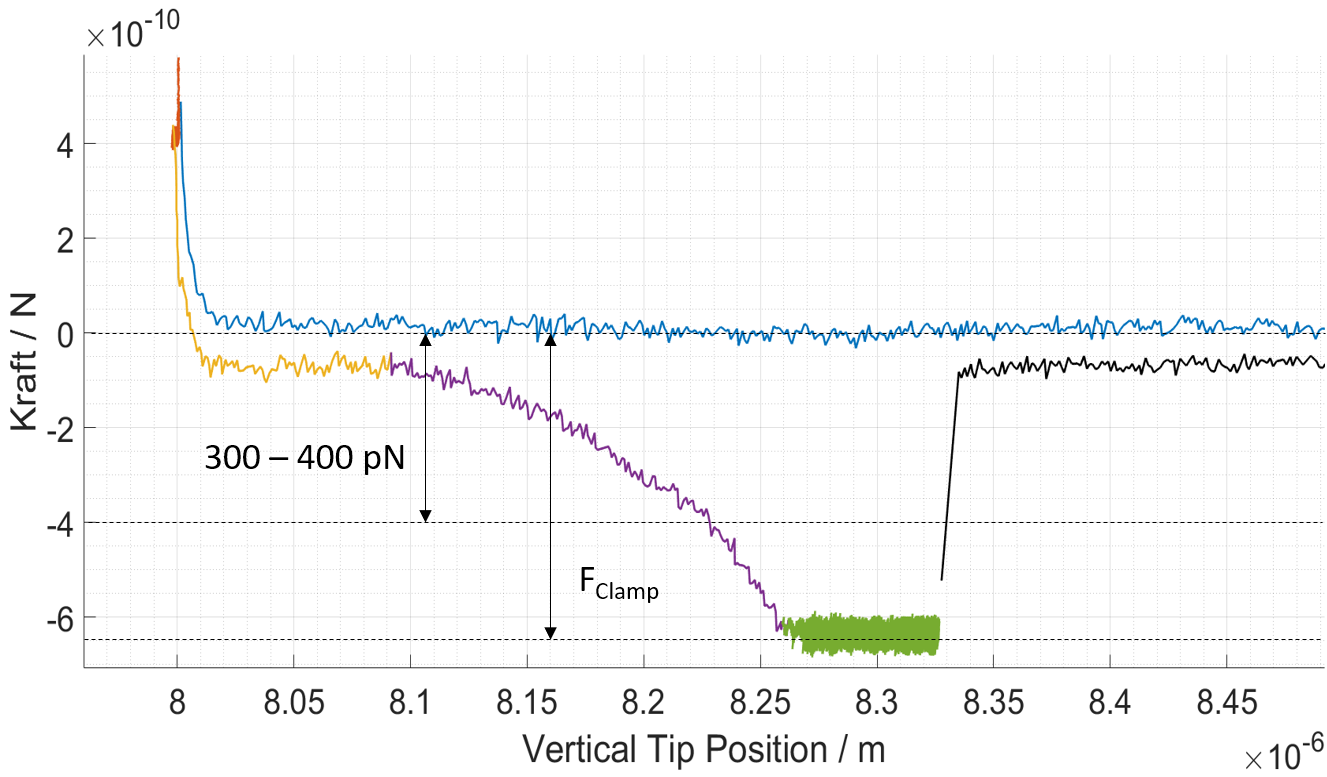
\includegraphics[width=\textwidth]{Abbildungen/Bsp_Force_Clamp_F_vs_x_IV.png}
		} % scalebox
		\subcaption{}
		\label{subfig:kraft_abstand}		
	\end{subfigure}
	\begin{subfigure}[b]{\textwidth}
		\centering
		\scalebox{\hscaleZero}{
			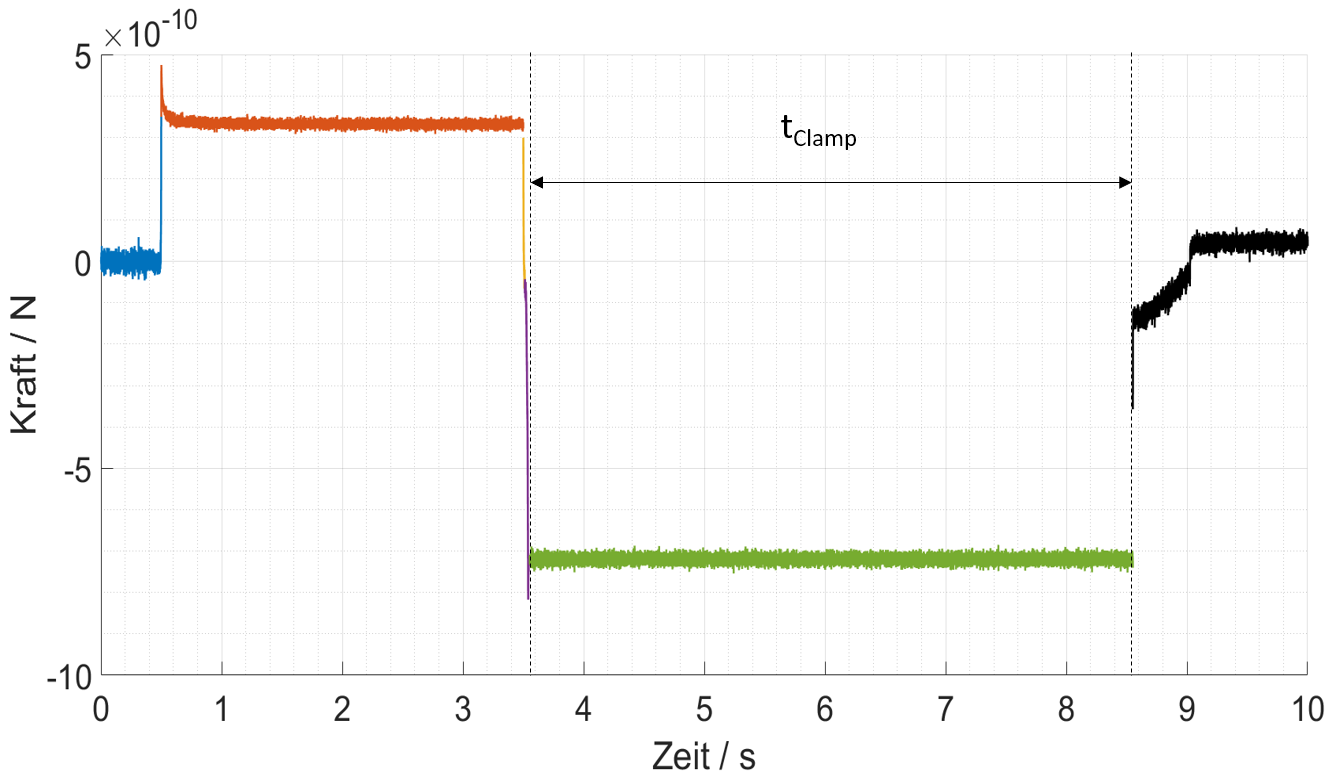
\includegraphics[width=\textwidth]{Abbildungen/Bsp_Force_Clamp_F_vs_t_III.png}
		} % scalebox
		\subcaption{}
		\label{subfig:kraft_zeit}			
	\end{subfigure}
	\caption[Beispiele einer Force-Clamp-Kraftkurve]{Beispiele einer Force-Clamp-Kraftkurve: a) Kraft-Abstand-Kurve. Hervorgehoben ist das \acs*{CMA}-spezifische Plateau bei 300 - 400 pN. b) Kraft-Zeit-Kurve. Hervorgehoben ist die Clampzeit dieser Kraftkurve von $t_{Clamp}~=~5,02~s$. Blau: Hinfahrkurve. Orange: Ruhezeit. Gelb: Initial Retract. Lila: Clamp Retract. Grün: Retract. Schwarz: Retract.}
	\label{fig:force_clamp_kurve}
\end{figure}

\subsection{Auflösungsgrenzen der Kraftexperimente}
\label{subsec:auflösungsgrenzen_der_kraftexperimente}

Über die \samplerate~wird bestimmt, mit welcher Datenauflösung Force-Clamp-Experimente in den einzelnen Domänen (Zeit, Weg und Kraft) aufgenommen werden können. Datenauflösung bedeutet in diesem Zusammenhang, wie klein ein bestimmtes Intervall (Zeitintervall, Wegintervall oder Kraftintervall) sein darf, sodass eine Mindestanzahl von Datenpunkten nicht unterschritten wird. Die \samplerate~ist folgendermaßen definiert:

\begin{equation}
	f_r = \frac{Datenpunkte}{Zeitintervall} = \frac{c}{\Delta t}
\end{equation}

Für die \samplerate~gilt:

\[ \frac{c}{\Delta t} = \frac{c_{min}}{\Delta t_{min}} \]

Damit folgt für das kleinste Zeitintervall:

\begin{equation}
	\Delta t_{min} = c_{min} \cdot \frac{\Delta t}{c} =  \frac{c_{min}}{f_r}
\end{equation}

Für mindestens einen Datenpunkt in $\Delta t_{min}$, muss $c_{min} = 1$ gelten:

\begin{equation}
		\Delta t_{min} = \frac{1}{f_r}
\end{equation}

$\Delta t_{min}$ kann über die Zuggeschwindigkeit $v$ in das minimale Wegintervall $\Delta l_{min}$ umgerechnet werden:

\begin{equation}
	\Delta l_{min} = v \cdot \Delta t_{min} = v \cdot \frac{c_{min}}{f_r}
\end{equation}

Für $\Delta l_{min}$ gilt ebenfalls $c_{min} = 1$:

\begin{equation}
	\Delta l_{min} = \frac{v}{f_r}
\end{equation}

 $\Delta l_{min}$ kann wiederum über die Federkonstante des Cantilevers $k_{Spring}$, in das minimale Kraftintervall $\Delta F_{min}$ umgerechnet werden:

\begin{equation}
	\Delta F_{min} = k_{Spring} \cdot \Delta l_{min} = k_{Sping} \cdot v \cdot \Delta t_{min} = \frac{k_{Spring} \cdot v}{f_r} \cdot c_{min}
\end{equation}

Für $\Delta F_{min}$ muss ebenfalls $c_{min} = 1$ gelten:

\begin{equation}
	\Delta F_{min} = \frac{k_{Spring} \cdot v}{f_r}
\end{equation}

Typische Werte für $f_r$, $v$\footnote{$v$ bezieht sich auf das 5. Segment (Clamp-Retract) eines Force-Clamp-Experiments. In diesem Segment wurde die \amid~bis auf die vorgesehene Kraft ($800~pN$) gestreckt.} und $k$ sind:

\begin{itemize}
	\item $f_r = 5000~s^{-1}$
	\item $v~= 5~µms^{-1}$
	\item $k_{Spring} = 0,08~Nm^{-1}$
\end{itemize}

Daraus ergeben sich für die jeweiligen Auflösungsgrenzen die folgenden Werte:

\begin{itemize}
	\item $\Delta t_{min} = \frac{1}{f_r} = \frac{1}{5000~s^{-1}} = 0,2 ms$
	\item $\Delta l_{min} = \frac{v}{f_r} = \frac{5 \cdot 10^{-6}~ms^{-1}}{5000~s^{-1}} = 1 \cdot 10^{-9}~m = 1~nm$
	\item $\Delta F_{min} = \frac{k_{Spring} \cdot v}{f_r} = \frac{0,08~Nm^{-1} \cdot 5 \cdot 10^{-6}~ms^{-1}}{5000~s^{-1}} = 8 \cdot 10^{-11}~N = 80~pN$
\end{itemize}
	\chapter{Material und Methoden}
\label{kap:material_und_methoden}

\section{Material}
\label{sec:material}

\subsection{Chemikalien}
\label{subsec:chemikalien}

\begin{table}[H]
	\centering
	\keepXColumns
	\caption{Auflistung der verwendeten Chemikalien.}
	\begin{tabularx}{\textwidth}{X X}
		\textbf{Bezeichnung}	&	\textbf{Bezogen von}	\\
		\toprule
		\toprule
		\ac{EDC}	&	Sigma Aldrich	\\
		&\\
		\ac{NHS}	&	Sigma Aldrich	\\
		&\\
		\ac{CMA}	&	Santa Cruz Biotechnologie	\\
		&\\
		\ac{PBS}	&	Biochrom	\\
		&\\
		Ethanol 99\% unvergällt	&	Carl Roth	\\
		&\\
		\ac{HCl} (32 \%)	&	Carl Roth	\\
		&\\
		\ac{NaOH}	&	Carl Roth	\\
		&\\
		Allylamin	&	Sigma Aldrich	\\
		&\\
		Vitamin E	&	Sigma Aldrich	\\
		\toprule
		\toprule
	\end{tabularx}
	\label{tab:chemikalien}
\end{table}

Alle Chemikalien wurden vor der Verwendung, falls nicht anders vermerkt, nicht weiter bearbeitet. \acs*{CMA} steht bei Santa Cruz Biotechnology seit Juli 2017 nicht mehr im Sortiment.

\subsection{Substrate}
\label{subsec:substrate}

\begin{table}[H]
	\centering
	\keepXColumns
	\captionabove{Auflistung der verwendeten Substrate.}
	\begin{tabularx}{\textwidth}{X X}		
		\textbf{Bezeichnung}	&	\textbf{Bezogen von}	\\
		\toprule
		\toprule
		GE Window DLC-Substrates	&	UQG Optics	\\
		&\\
		NPG-10 Cantilever mit HDC Spitzen	&	Bruker/ Nanotools	\\
		\toprule
		\toprule
	\end{tabularx}
	\label{tab:substrate}
\end{table}

Das GE-Window ist ein drei mm dickes Germanium-Glass-Substrat, beschichtet mit sieben µm \ac{DLC}. Die NPG-10 Cantilever von Bruker wurden von Nanotools mit einer \ac{HDC} Spitze modifiziert.

\subsection{Geräte und Software}
\label{subsec:geräte_und_software}

\begin{table}[H]
	\centering
	\keepXColumns
	\captionabove{Auflistung von verwendeten Geräten und verwendeter Software.}
	\begin{tabularx}{\textwidth}{X X}
		\textbf{Bezeichnung}	&	\textbf{Hersteller}	\\
		\toprule
		\toprule
		Nanowizard I\textsuperscript{\textregistered}	&	JPK Instruments AG	\\
		&\\
		UV Penray ($\lambda = 254~nm$)	&	UVP, LLC	\\
		&\\
		MATLAB	&	Mathworks	\\
		\toprule
		\toprule
	\end{tabularx}
	\label{tab:geräte_software}
\end{table}

\section{Methoden}
\label{sec:methoden}

\subsection{Oberflächenfunktionalisierung der Substrate}
\label{subsec:oberflächenfunktionalisierung_der_substrate}

Bei der gesamten Handhabung der \spitzen~war auf einen adäquaten Schutz vor elektrostatischer Entladung zu achten. Aus diesem Grund wurde mit den \spitzen~auf einer Schutzmatte gegen Elektrostatische Entladung gearbeitet. Zur persönlichen Schutzausrüstung gehörte zusätzlich ein Erdungsarmband. Um Beschädigung des Cantilevers zu vermeiden, wurde der gesamte $Si_3N_4$-Chip seitlich um 90° verkippt durch Flüssigkeitsgrenzflächen geführt. Bevor eine Funktionalisierung gestartet werden konnte, wurden \spitzen~und Substrate von organischen Verunreinigungen befreit. Die \spitzen~wurden dazu 90 min mit einer UV-Lampe beleuchtet, während die Substrate für diese Zeit in einer 5\% Hellmannex-Lösung im Ultraschallbad behandelt wurden. Die Substrate wurden anschließend für weitere 10 min mit doppelt destilliertem Wasser im Ultraschallbad gespült. Um die \spitzen~und Subrate mit terminalen \aminos~zu modifizieren wurde folgendes Protokoll verwendet:

\subsubsection{Präparation der Funktionalisierungslösungen}
\label{subsubsec:präparation_der_funktionalisierungslösungen}

\spitzen~und Substrate wurden in getrennten Glasgefäßen (ca. 3 ml Volumen) funktionalisiert. Die Ansätze beider Gefäße setzten sich jeweils aus ca. 2,7 ml reinem Ethanol (eingefüllt \textit{via} Tropfpipette) und ca. 0,3 ml Allylamin (eingefüllt \textit{via} 1 ml Spritze mit Kanüle des Durchmessers 0,9 mm) zusammen. Nach dem Vorlegen von Allylamin wurde anschließend Ethanol hinzugegeben. Der Ansatz wurde durch dreimaliges \enquote{auf und ab pipettieren} mit der Tropfpipette durchmischt.

\subsubsection{Oberflächenfunktionalisierung}
\label{subsubse:oberflächenfunktionalisierung}

Gereinigte \spitzen~und Substrate wurden in jeweils ein Gefäß mit einem Funktionalisierungsansatz gegeben. Zum Starten der Oberflächenfunktionalisierung, wurden beide Ansätze in eine UV-Kammer gegeben und unter Stickstoffbegasung mit einer UV-Lampe ($\lambda = 254~nm$) über eine Zeit von 3 Stunden bestrahlt.

\subsubsection{Stoppen der Funktionalisierung}
\label{subsubsec:stoppen_der_oberflächenfunktionalisierung}

Die Oberflächenfunktionalisierung wurde in einer Vitamin-E Lösung gestoppt, wobei das Vitamin-E als Radikalfänger diente. Zur Herstellung der Vitamin-E Lösung wurde in eine Petrischale, gefüllt mit reinem Ethanol, eine Spatelspitze Vitamin-E durch Rühren gelöst. Zum Stoppen der Funktionalisierung wurden \spitzen~und Substrate für zwei Minuten in die Lösung gegeben und anschließend in ein zweites Gefäß mit reinem Ethanol überführt.

\subsubsection{Entfernen nicht gebundener Reaktanden}
\label{subsubsec:entfernen_nicht_gebundener_reaktanden}

Um ungebundenes Allylamin von den Oberflächen der \spitzen~und Substrate zu entfernen, wurden \spitzen~und Substrate getrennt voneinander gereinigt. Die Substrate wurden in ein Becherglas, gefüllt mit einer 1:2 Verdünnung aus reinem Ethanol und doppelt destilliertem Wasser, gegeben und für insgesamt 40 Minuten in einem Ultraschallbad gereinigt. Die \spitzen~ruhten in dieser Zeit in reinem Ethanol. Substrate, sowie \spitzen~wurden anschließend für ca. 5 Minuten an Luft getrocknet. Zur Lagerung wurden \spitzen~und Substrate in einen Exsikkator mit Trocknungsmittel (Silicagel) gegeben.

\subsection{Vorbereitung der Versuche}
\label{subsec:vorbereitung_der_versuche}

\subsubsection{Präparation der Kopplungslösungen}
\label{subsubsec:präparation_der_kopplungslösungen}

Zunächst wurde eine \ac{CMA}-Lösung hergestellt. Dazu wurden 1 mg \ac{CMA} mit 0,1 ml \ac{PBS} mit einem pH-Wert von 6,5 (der pH-Wert wurde mit 32 \% \ac{HCl} eingestellt) gelöst. Dazu wurde der Ansatz in ein 1,5 ml Zentrifugenröhrchen gegeben und auf einem Vortexer für 20 min fixiert.\\
Anschließend wurde eine \ac{EDC}/ \ac{NHS}-Lösung hergestellt. Dazu wurden 10 mg \ac{NHS} und 25 mg \ac{EDC} in einem 1,5 ml Zentrifugenröhrchen, in 0,5 ml derselben \ac{PBS}-Lösung wie oben, auf einem Vortexer für ca. 10 Sekunden gemischt.\\
Zur Herstellung der Kopplungslösung wurden 0,1 ml der \ac{EDC}/ \ac{NHS}-Lösung mit 0,1 ml der \ac{CMA}-Lösung gemischt, sodass die \ac{CMA}-Konzentration bei ca. 5 mg/ml lag.

\subsubsection{Kopplung der Spacer an die Substrate}
\label{subsubsec:kopplung_der_spacer_an_die_substrate}

Die Kopplung von \spacer~mit dem Substrat bzw. \spitze~geschah durch nachfolgende Sequenz:

\begin{enumerate}
	\renewcommand\labelenumi{\bfseries\theenumi.}
	
	\item Beschichten des Substrates mit 30 \% Essigsäure \textit{via} Tropfpipette für 3 min.
	\item Entfernen der Essigsäure durch abpipettieren \textit{via} Tropfpipette und Zugabe von ca. 50~µl der Kopplungslösung für 10 min.
	\item Entfernen der Kopplungslösung durch dreifaches Spülen mit jeweils 1~ml der \ac{PBS}-Lösung aus dem vorherigen Abschnitt.
	\item Hinzufügen von ca. 50 µl der \ac{EDC}/ \ac{NHS}-Lösung aus dem vorherigen Abschnitt,  für 3 min.
	\item Auffüllen der Petrischale mit \ac{PBS} des gewünschten pH-Wertes\footnote{Die pH-Werte wurden mit einer 1M NaOH-Lösung oder mit 32\% \ac{HCl} eingestellt.} bis die Oberfläche des Substrates ca. 2 bis 5 mm unterhalb des Flüssigkeitsmeniskus lag.
	
\end{enumerate}

Anschließend wurden die Messungen am \ac{AFM} gestartet.

\subsection{Durchführung der Versuche}
\label{subsec:durchführung_der_versuche}

Die Durchführung aller Versuche gliederte sich in drei Abschnitte:

\begin{enumerate}
	\renewcommand\labelenumi{\bfseries\theenumi.}
	
	\item Kalibrierung des Cantilevers
	\item Auswahl der x,y-Position auf dem Substrat 
	\item Start des Force-Clamp-Experiments
	
\end{enumerate}

\subsubsection{Kalibrierung des Cantilevers}
\label{subsubsec:kalibrierung_des_cantilevers}

Die Kalibrierung des Cantilevers diente der Umrechnung der Cantileverauslenkung von Einheiten der Spannung in Einheiten der Kraft. Die Kalibrierung erfolgte in zwei Schritten. Zunächst wurde die optische Sensitivität des Cantilevers ermittelt. Dies diente der Umrechnung des Spannungssignals an der Photodiode in die Auslenkung des Cantilevers in Einheiten der Länge. Anschließend wurde die Federkonstante des Cantilevers über die Methode des thermischen Rauschens bestimmt \cite{Butt.1995}. Über die Federkonstante wurde die Cantileverauslenkung in Einheiten der Kraft umgerechnet. Eine detaillierte Anleitung des Ablaufs kann in der Arbeit von T.Becke \textit{et al.} \cite{Becke.2018} nachgeschlagen werden.\\
Nach der Kalibrierung mussten die Regelparameter des \acp{AFM} (Integralwert und Proportionalwert) an das System angepasst werden.

\subsubsection{Auswahl der x,y-Position des Force-Clamp-Experiments auf dem Substrat}
\label{subsubsec:auswahl_der_x_y_position_des_force_clamp_experiments_auf_dem_substrat}

Zunächst wurden die \spitzen~mittels einer Topview-Kamera auf die Mitte des Substrats ausgerichtet. Um zu verifizieren, ob an dieser Stelle Einzelmolekülinteraktionen zwischen \spitze~bzw. Substrat und \spacer~auftraten, wurde zuerst ein Force-Ramp-Experiment durchgeführt. Falls keine entsprechenden Interaktionen zu beobachten waren, wurde der Cantilever auf eine andere Stelle des Substrats ausgerichtet. Da die \ester~in Lösung nicht unbegrenzt stabil waren \cite{Hayworth}, wurde die Verifizierung der Position in maximal 30 min durchgeführt. Dazu wurde mittels der \ac{AFM}-Software ein quadratisches Raster mit einer Kantenlänge von $100~\mu m$ und 5 Messpunkte pro Achse (insgesamt 25 Messpunkte) programmiert und abgefahren. Details der Force-Ramp-Experimente können der Tabelle~\ref{tab:force-ramp-parameter} entnommen werden. Eine ausführliche Beschreibung der Force-Ramp-Experimente erfolgte in Abschnitt~\ref{subsec:kraftkurven}

\subsubsection{Start des Force-Clamp-Experiments}
\label{subsubsec:start des force-clamp-experiments}

Nachdem Auswählen einer passenden Stelle auf dem Substrat, wurde das Force-Clamp-Experiment durchgeführt. Um möglichst viele Einzelmolekülinteraktionen zu messen, wurden die Messpunkte des vorherigen Rasters auf 10 pro Achse (insgesamt 100 Messpunkte) erhöht. Jeder Messpunkt wurde zudem dreimal angefahren. Damit erhöhte sich die Messdauer auf 2,5 Stunden. Eine Anpassung der Parameter für verschiedene Experimente war nur im 3. Segment nötig. Hier wurde die Länge des Initial Retract für jedes Paar aus \spitze~und Substrat während des Experiments neu bestimmt. Die Länge schwankte dabei von $100$ bis $500~nm$. Details der Force-Clamp-Experimente können aus Tabelle~\ref{tab:force-clamp-parameter} entnommen werden. Eine ausführliche Beschreibung der Force-Clamp-Experimente erfolgte in Abschnitt~\ref{subsec:kraftkurven}.


\begin{table}[H]
	\centering
	\keepXColumns
	\captionabove{Experimenteller Ablauf der Force-Ramp-Experimente.}
	\begin{tabularx}{\textwidth}{X X X X}
		\multicolumn{2}{l}{\textbf{Parameter}}	&	\textbf{Einheit}	&	\textbf{Wert}	\\
		\toprule
		\toprule
		\multicolumn{4}{c}{Scanbereich}	\\
		\toprule
		\multicolumn{2}{l}{Scanfläche}	&	$\mu m^2$	&	100x100	\\
		&&&\\
		\multicolumn{2}{l}{Punkte/ Achse}	&	1	&	5	\\
		&&&\\
		\multicolumn{2}{l}{Messungen/ Punkt}	&	1	&	1	\\
		&&&\\
		\multicolumn{2}{l}{Dauer der Force-Maps}	&	$h$	&	0.5	\\
		&&&\\
		\toprule
		\multicolumn{4}{c}{Experimentelles Setup}	\\
		\toprule
		\multirow{5}{3cm}{1. Hinfahrkurve}	&	Setpoint	&	$pN$	&	250	\\
		&&&\\
		&	z-Länge	&	$\mu m$	&	3	\\
		&&&\\
		&	z-Geschwindigkeit	&	$\mu m/s$	&	6	\\
		\toprule
		\multirow{3}{3cm}{2. Ruhezeit}	&	Setpoint	&	$pN$	&	250	\\
		&&&\\
		&	Dauer	&	$s$	&	3	\\
		\toprule
		\multirow{3}{3cm}{3. Wegfahrkurve}	&	z-Länge	&	$\mu m$	&	3	\\
		&&&\\
		&	z-Geschwindigkeit	&	$\mu m/s$	&	6 \\
		\toprule
		\toprule
	\end{tabularx}
	\label{tab:force-ramp-parameter}
\end{table}

\begin{table}[H]
	\centering
	\keepXColumns
	\captionabove{Experimenteller Ablauf der Force-Clamp-Experimente.}
	\begin{tabularx}{\textwidth}{X X X X}
		\multicolumn{2}{l}{\textbf{Parameter}}	&	\textbf{Einheit}	&	\textbf{Wert}	\\
		\toprule
		\toprule
		\multicolumn{4}{c}{Scanbereich}	\\
		\toprule
		\multicolumn{2}{l}{Scanfläche}	&	$\mu m^2$	&	100x100	\\
		&&&\\
		\multicolumn{2}{l}{Punkte/ Achse}	&	1	&	10	\\
		&&&\\
		\multicolumn{2}{l}{Messungen/ Punkt}	&	1	&	3	\\
		&&&\\
		\multicolumn{2}{l}{Dauer der Force-Map}	&	$h$	&	2	\\
		&&&\\
		\toprule
		\multicolumn{4}{c}{Experimentelles Setup}	\\
		\toprule
		\multirow{5}{3cm}{1. Hinfahrkurve}	&	Setpoint	&	$pN$	&	250	\\
		&&&\\
		&	z-Länge	&	$\mu m$	&	3	\\
		&&&\\
		&	z-Geschwindigkeit	&	$\mu m/s$	&	6	\\
		\toprule
		\multirow{3}{3cm}{2. Wartezeit}	&	Setpoint	&	$pN$	&	250	\\
		&&&\\
		&	Dauer	&	$s$	&	3	\\
		\toprule
		\multirow{3}{3cm}{3. Initial Retract}	&	z-Länge	&	$\mu m$	&	0,1 bis 0,5	\\
		&&&\\
		&	z-Geschwindigkeit	&	$\mu m/s$	&	5	\\
		\toprule
		\multirow{5}{3cm}{4. Clamp-Retract}	&	Setpoint	&	$pN$	&	-800	\\
		&&&\\
		&	z-Länge	&	$\mu m$	&	1	\\
		&&&\\
		&	z-Geschwindigkeit	&	$\mu m/s$	&	5	\\
		\toprule
		\multirow{3}{3cm}{5. Clamp}	&	Setpoint	&	$pN$	&	-800	\\
		&&&\\
		&	maximale Dauer	&	$s$	&	30	\\
		\toprule
		\multirow{3}{3cm}{6. Retract}	&	z-Länge	&	$\mu m$	&	3	\\
		&&&\\
		&	z-Geschwindigkeit	&	$\mu m/s$	&	6	\\
		\toprule
		\toprule
	\end{tabularx}
	\label{tab:force-clamp-parameter}
\end{table}

\subsection{Kategorisierung der Kraftkurven}
\label{subsec:kategorisierung_der_kraftkurven}

Um die Auswertung der aufgenommenen Kraftkurven zu erleichtern, wurden diese in verschiedene Kategorien eingeteilt. Die Kategorisierung wurde nach dem Schema, dargestellt in \abb~\ref{fig:kategorisierung}, durchgeführt.\\
Im ersten Schritt wurde anhand der Kraft-Zeit-Kurve nachgeprüft, ob die eingestellte Clampkraft von $800~pN$ für mindestens $100~ms$ gehalten wurde. Anschließend erfolgte die Einteilung der Kraft-Abstands-Kurve in die Kategorien A bis E. Die Kategorien sind dabei wie folgt definiert

\begin{figure}[h]
	\centering
	\scalebox{\hscaleZero}{
		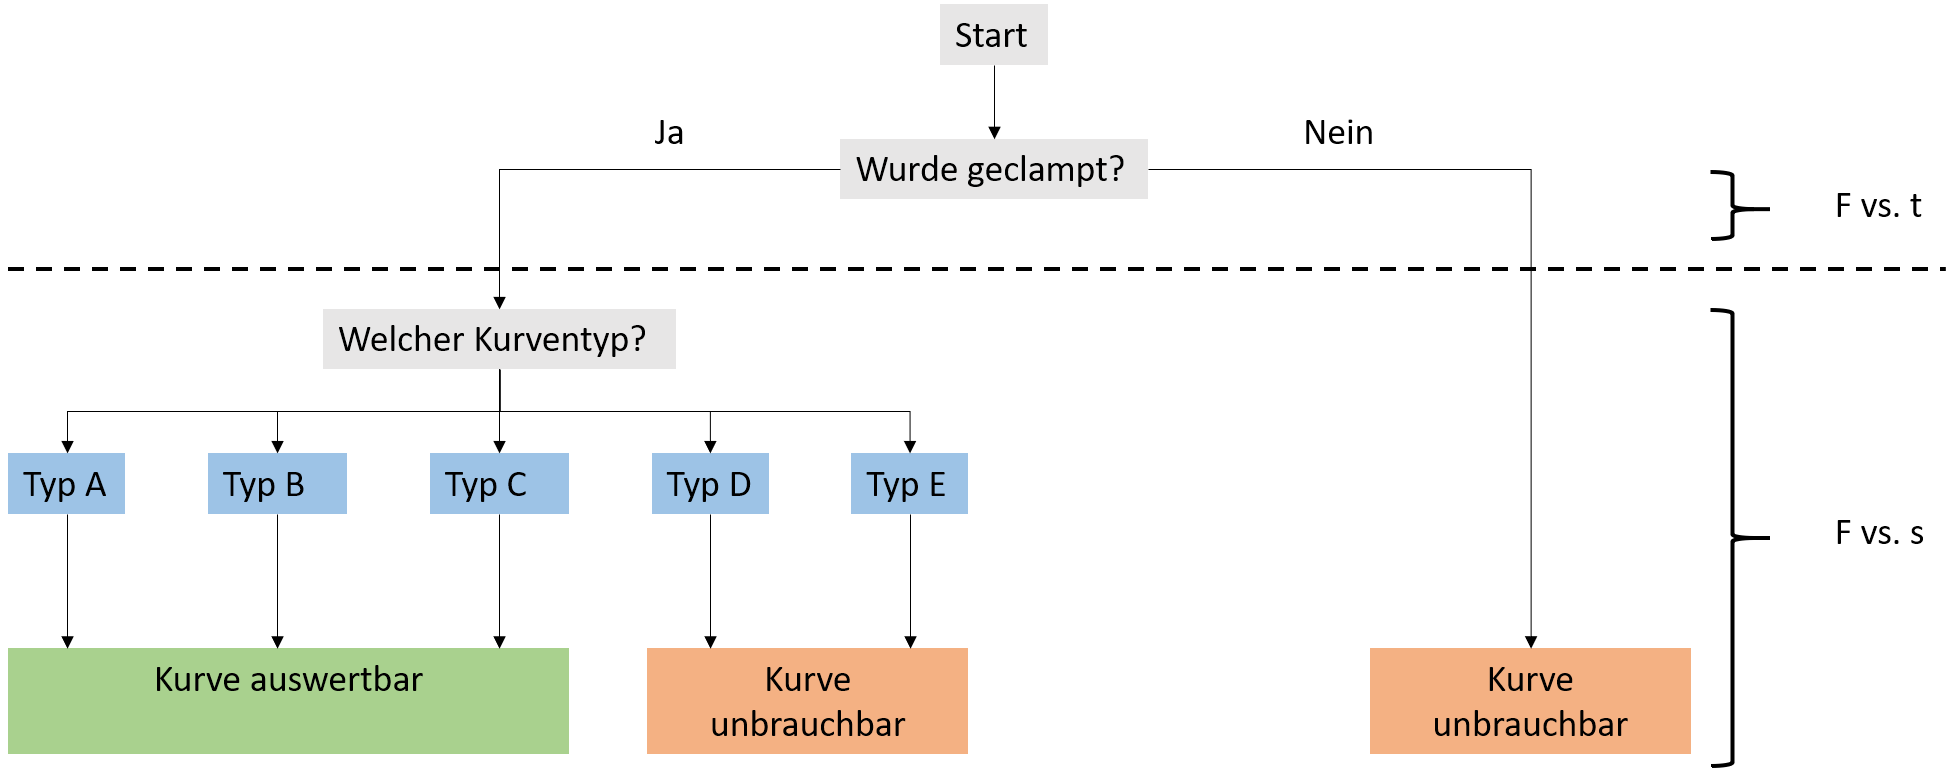
\includegraphics[width=\linewidth]{Abbildungen/Auswertung_ueberblick_VI.png}
	} % scalebox
	\caption[Ablaufschema der Kategorisierung]{Ablauf der Kategorisierung. Auswertbare Kraftkurven (Kategorie A und B) durften zusätzlich nicht bis zur maximalen Clampzeit gehalten werden oder einen Doppelpeak aufweisen. Die Kategorisierung erfolgte in zwei Schritten. Zunächst wurde anhand der Kraft-Zeit-Kurve (F vs. t) bestimmt ob ein Clampereigniss stattfand. Danach wurden die Kraftkurven in der Kraft-Abstand Darstellung (F vs. s) in die jeweiligen Kategorien eingeteilt.}
	\label{fig:kategorisierung}
	
\end{figure}

\subsubsection{Kategorie A}
\label{subsubsec:kategorie_a}

Kraftkurven dieser Kategorie wiesen während der gesamten Wegfahrkurve einen einzelnen Abriss auf. Dieser galt als Einzelmolekülinteraktion, wenn das für \ac{CMA} typische Plateau bei $300-400~pN$ zu erkennen war. In \abb~\ref{fig:kategoire_a_kurve} ist eine Kategorie A Kraftkurve dargestellt. Kurven aus dieser Kategorie konnten ohne weiteres in die Auswertung mit aufgenommen werden, da während des gesamten Experiments kein weiterer Abriss (insbesondere kürzere Abrisse) das Ereignis beeinflussten. In einigen Fällen kam es vor, dass bei besonders kurzen Abrissen ($< 300~nm$), kein Plateau sichtbar war. Solche Kurven wurden dennoch zur Kategorie A gezählt.

\begin{figure}[H]
	\centering
	\scalebox{\hscaleZero}{
		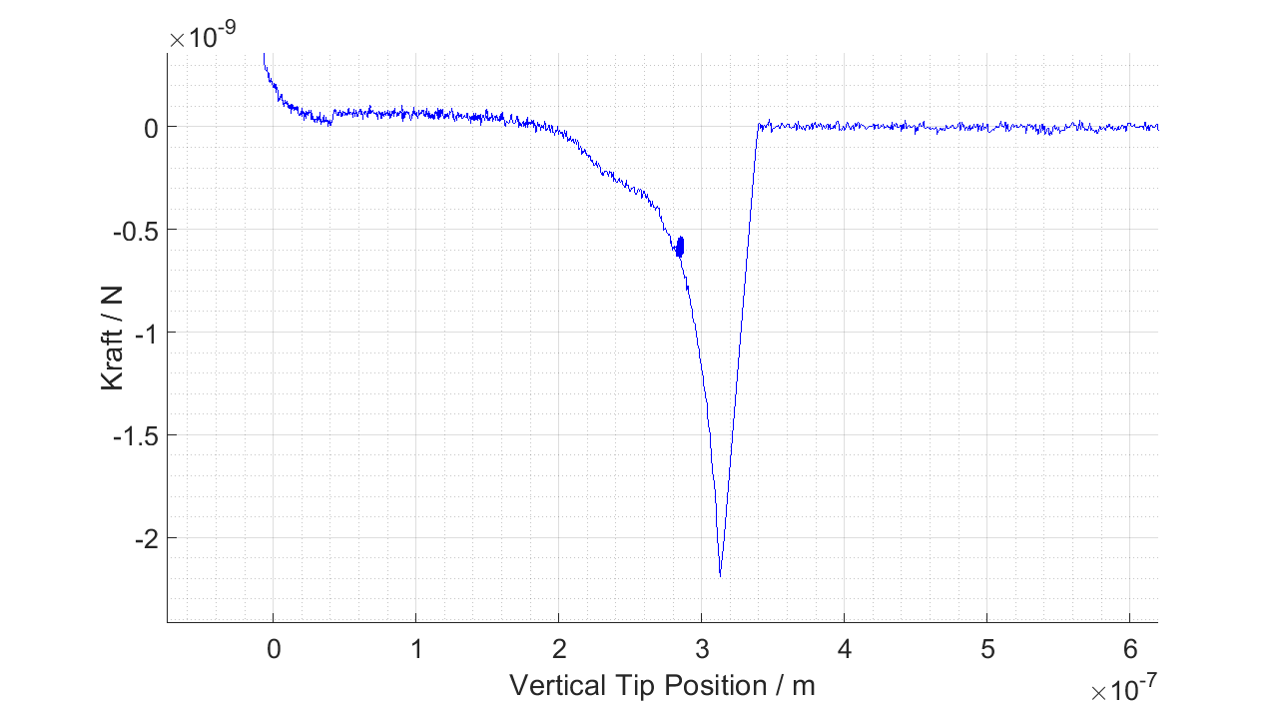
\includegraphics[width=\linewidth]{Abbildungen/Kategorien/A_I.png}
	} % scalebox
	\caption[Beispiel einer Kategorie A Kraftkurve]{Beispiel einer Kategorie A Kraftkurve. Diese Kurve zeigt das typische Plateau in einem Kraftbereich von 300 - 400 pN.}
	\label{fig:kategoire_a_kurve}
\end{figure}

\subsubsection{Kategorie B}
\label{subsubsec:kategorie_b}

Diese Kategorie wies in der Wegfahrkurve vor dem Hauptabriss (Peak bei der größten Abrisskraft) einen oder mehrere, vorgelagerte Abrisse bei einer Kraft von ca. $10-100~pN$ auf. Ein typisches Beispiel aus dieser Kategorie zeigt \abb~\ref{fig:kategorie_b_kurve}. Einzelmolekülinteraktionen aus dieser Kategorie konnten in vollem Umfang zur Auswertung herangezogen werden, sofern, die vorgelagerten Peaks vor, oder direkt am Beginn des Hauptabrisses lagen. Auch hier wurden, analog zu Kategorie A, kurze Abrisse ($< 300~nm$) zur Kategorie B gezählt.

\begin{figure}[H]
	\centering
	\scalebox{\hscaleZero}{
		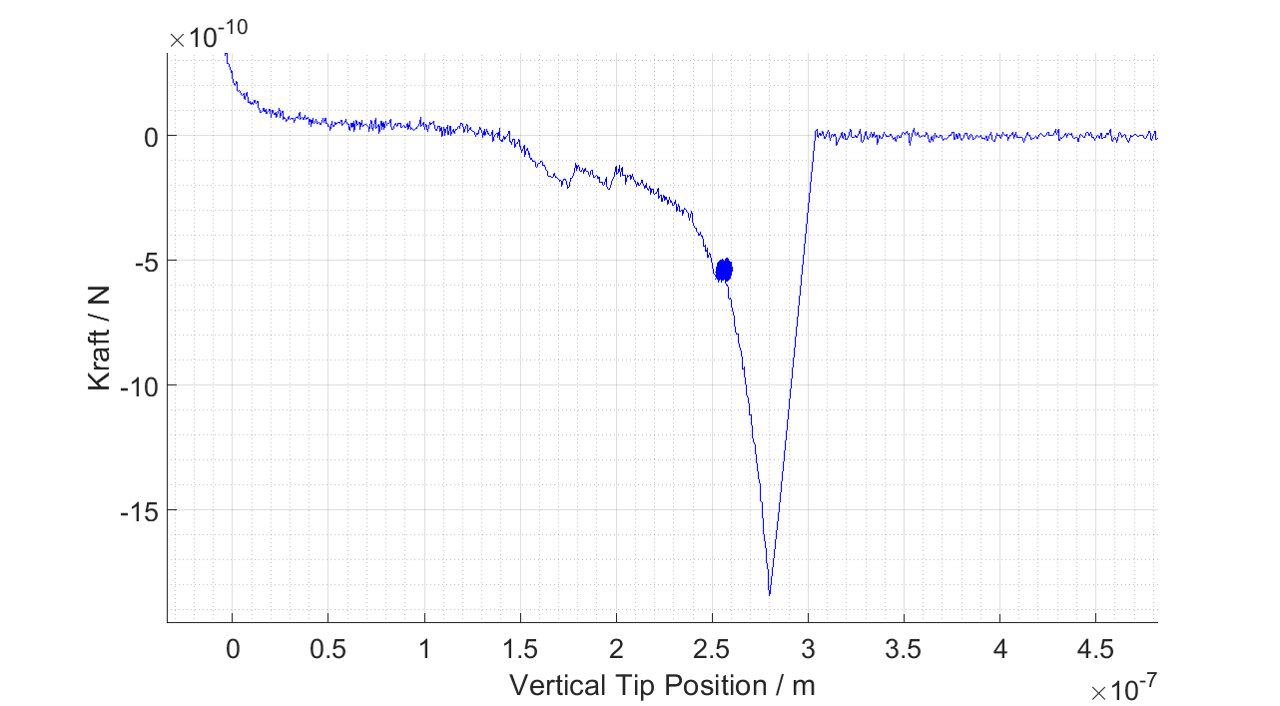
\includegraphics[width=\linewidth]{Abbildungen/Kategorien/BII.png}
	} % scalebox
	\caption[Beispiel einer Kategorie B Kraftkurve]{Beispiel einer Kategorie B Kraftkurve. Das typische Plateau von \acs*{CMA} bei 300 - 400 pN wird durch die, dem Hauptpeak vorgelagerten, kurzen Abrisse verdeckt. Die Vorgelagerten Abrisse liegen in der Größenordnung von 10 bis 100 pN.}
	\label{fig:kategorie_b_kurve}
\end{figure}

\subsubsection{Kategorie C}
\label{subsubsec:kategorie_c}

Dieser Kategorie wurden Kraftkurven zugeordnet, die in der Wegfahrkurve mehrere starke Abrisse (Abrisskraft lag im nN-Bereich) aufwiesen. Nicht alle Abrisse zeigten das \ac{CMA}-spezifische Plateau bei $300 - 400~pN$, starteten jedoch überwiegend von der gleichen Kraft. Das bedeutet, dass der Cantilever bis zu seiner Ausgangslage vor der Interaktion zurückkehrte und der nächste Abriss von der Nulllinie\footnote{Der Begriff Nulllinie wird im Abschnitt~\ref{subsec:auswertung_der_versuchsergebnisse} erläutert.} aus startete. Eine typische Kategorie C Kraftkurve zeigt \abb~\ref{fig:kategorie_c_kurve}. Kurven aus dieser Kategorie konnten nicht ausgewertet werden.

\begin{figure}[H]
	\centering
	\scalebox{\hscaleZero}{
		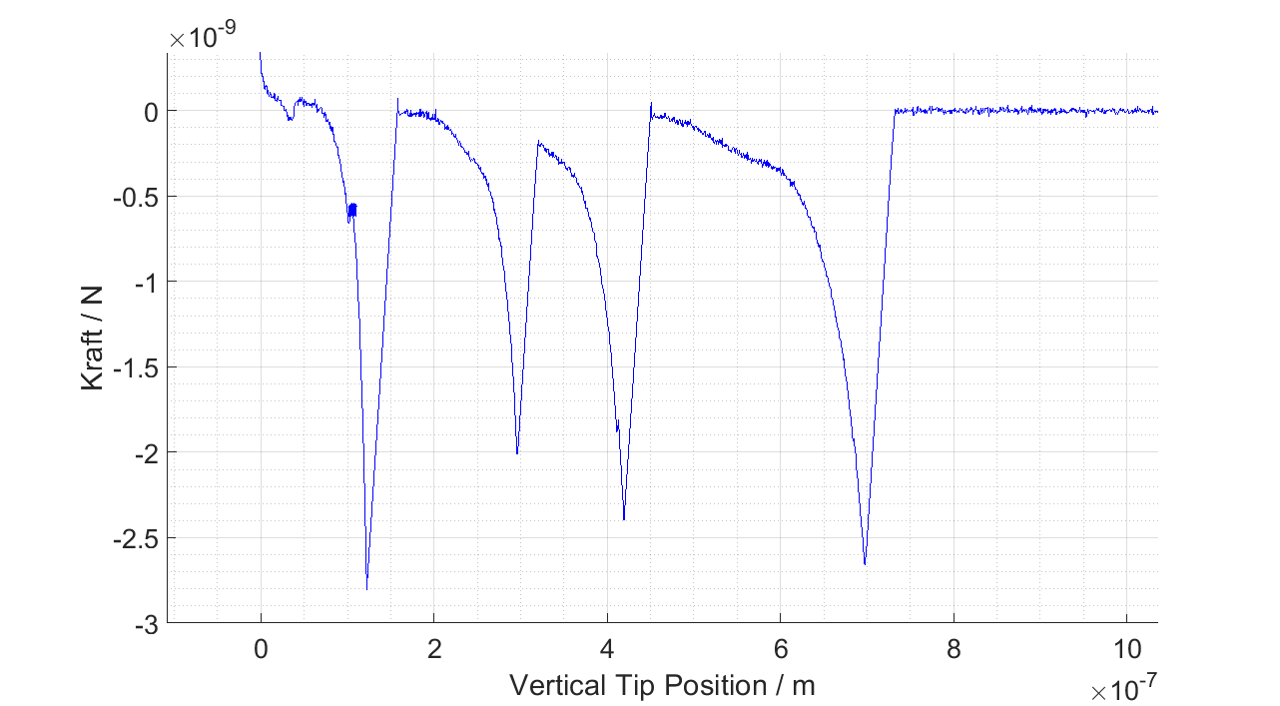
\includegraphics[width=\linewidth]{Abbildungen/Kategorien/CIII.png}
	} % scalebox
	\caption[Beispiel einer Kategorie C Kraftkurve]{Beispiel einer Kategorie C Kraftkurve. Alle aufeinander folgenden Abrisse beginnen in etwa bei der Nulllinie.}
	\label{fig:kategorie_c_kurve}
\end{figure}

\subsubsection{Kategorie D}
\label{subsubsec:kategorie_d}

Die Kurven aus dieser Kategorie wiesen in der Wegfahrkurve mehrere, überlagerte Abrisse auf. Typischerweise zeigten alle nachfolgenden Abrisse kein Plateau bei $300 - 400~pN$ und starteten bei höheren Kräften als der erste Abriss. Der Cantilever konnte zwischen den einzelnen Interaktionen nicht in seine Ausgangslage zurückkehren, sodass jeder weitere Abriss bei einer stärkeren Vorspannung auftreten musste. Ein typisches Beispiel einer Kategorie D Kraftkurve zeigt \abb~\ref{fig:kategorie_d_kurve}.

\begin{figure}[H]
	\centering
	\scalebox{\hscaleZero}{
		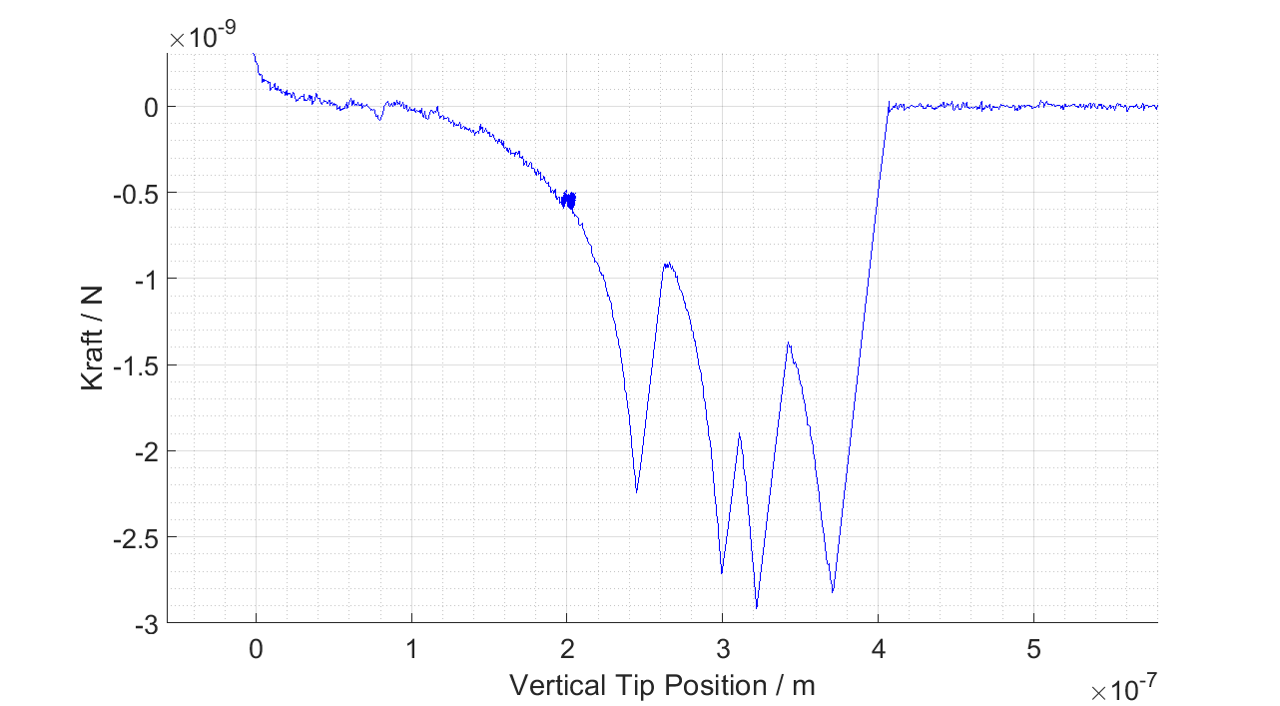
\includegraphics[width=\linewidth]{Abbildungen/Kategorien/DII.png}
	} % scalebox
	\caption[Beispiel einer Kategorie D Kraftkurve]{Beispiel einer Kategorie D Kraftkurve. Aufeinanderfolgende Abrisse starten bei einer höhere Kraft als die vorherigen Abriss. Es ist kein Plateau bei 300 - 400 pN zu erkennen.}
	\label{fig:kategorie_d_kurve}
\end{figure}

\subsubsection{Kategorie E}
\label{subsubsec:kategorie_e}

Diese Kategorie umfasst alle Kurven, welche nicht in eine der oberen Kategorien eingeordnet werden konnten. Typischerweise betraf das Kraftkurven mit ausschließlich unspezifischen Wechselwirkungen, wie beispielhaft in \abb~\ref{fig:kategorie_e_kurve} gezeigt wird.

\begin{figure}[H]
	\centering
	\scalebox{\hscaleZero}{
		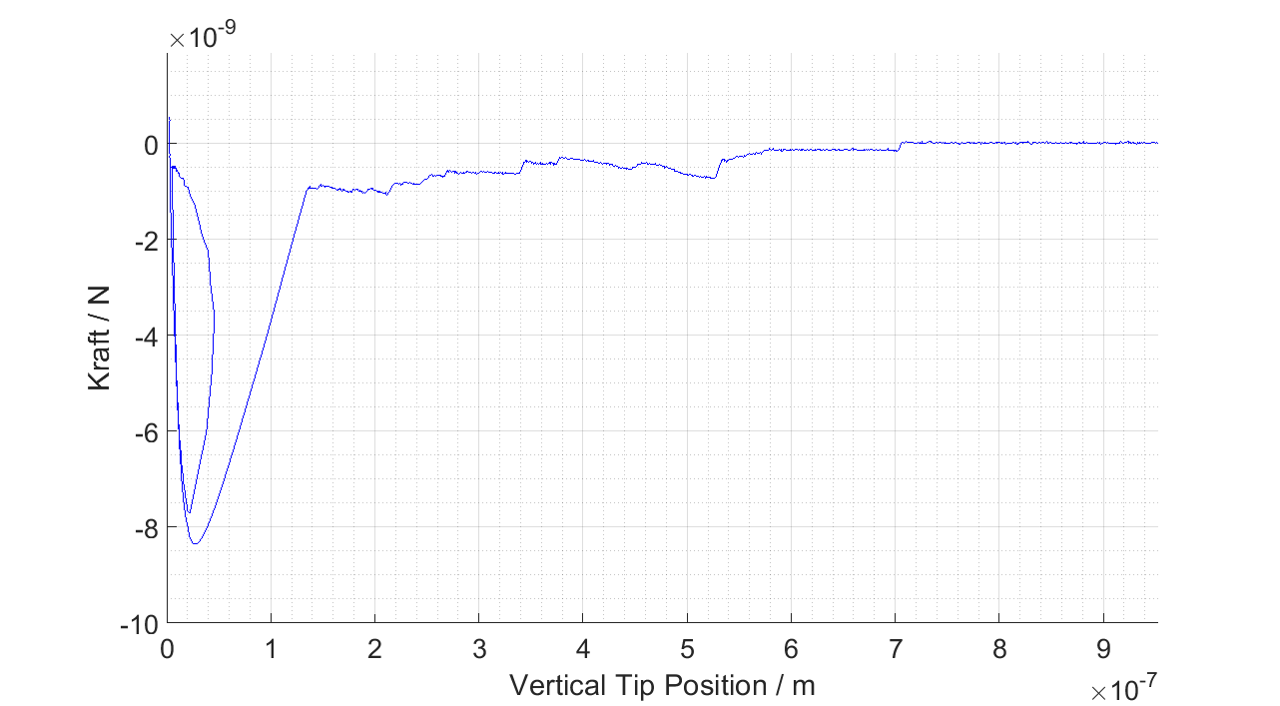
\includegraphics[width=\linewidth]{Abbildungen/Kategorien/EI.png}
	} % scalebox
	\caption[Beispiel einer Kategorie E Kraftkurve]{Beispiel einer Kategorie E Kraftkurve. Kraftkurve aus dieser Kategorie wiesen keine Merkmale auf, die eindeutig einer Einzelmolekülinteraktion mit \acs*{CMA} zuzuordnen waren.}
	\label{fig:kategorie_e_kurve}
\end{figure}

\subsubsection{Bemerkungen zu den Kraftkurven}
\label{subsubsec:bemerkungen_zu_den_kraftkurven}

Neben den eindeutig kategorisierbaren Details gab es Merkmale, welche in allen Kraftkurven auftreten konnten. Diese Merkmale beeinflussten nicht die Einordnung der Kraftkurven in die verschiedenen Kategorien (A bis E) und wurden während der Auswertung als Bemerkung zu jenen Messungen hinzugefügt.

\paragraph{Doppelpeak}
\label{par:doppelpeak}

Doppelpeaks gehörten prinzipiell zu Kraftkurven der Kategorie C, mit dem Unterschied, dass zwei direkt aufeinander folgende Peaks am Ende eines Abrisses sichtbar waren, wie in \abb~\ref{fig:doppelpeak} dargestellt. Doppelpeaks entstanden, wenn ein \ac{CMA}-Polymer unter Bildung einer Schlaufe (mehr als sechs Monomereinheiten) mehrfach an das Substrat oder die \spitze~gebunden haben. Den entsprechenden Kraftkurven wurde das Kürzel \ac{DP} hinzugefügt und wurden in der Auswertung ebenfalls nicht berücksichtigt.

\begin{figure}[H]
	\centering
	\scalebox{\hscaleZero}{
		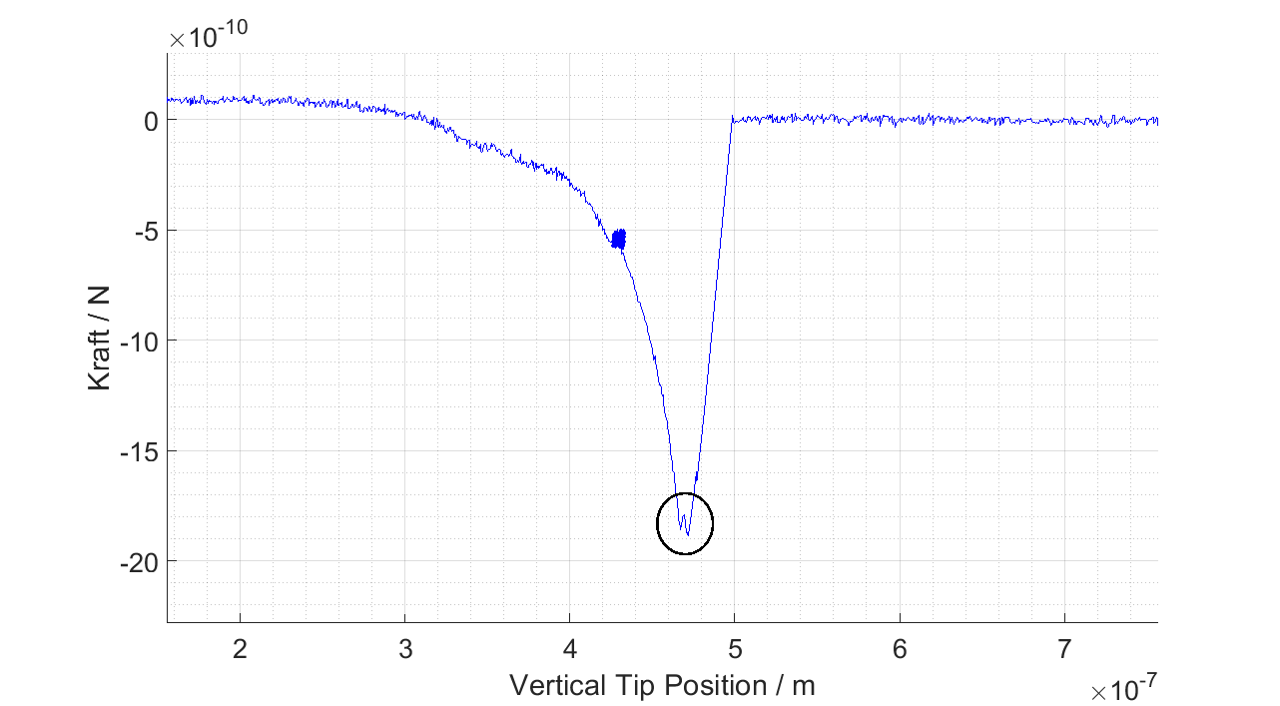
\includegraphics[width=\linewidth]{Abbildungen/Kategorien/DPII.png}
	} % scalebox
	\caption[Beispiel einer Kraftkurve mit Doppelpeak]{Beispiel einer Kraftkurve mit Doppelpeak.}
	\label{fig:doppelpeak}
\end{figure}

\paragraph{Maximale Clampzeit}
\label{par:maximale_clampzeit}

Es kam vor, dass einige Kurven bis zur maximal möglichen Clampzeit bei $800~pN$ gehalten werden konnten. Die Bindung wurde erst im 6. Segment der Force-Clamp-Experimente gebrochen. Kraftkurven mit dieser Besonderheit wurde das Kürzel \ac{tmax} hinzugefügt. Kraftkurven mit diesem Kürzel konnten nicht ausgewertet werden.

\subsection{Auswertung der Versuchsergebnisse}
\label{subsec:auswertung_der_versuchsergebnisse}

Die Messung der Abrisszeiten der aufgenommenen Kraftkurven wurde hauptsächlich mit der Data Processing Software von JPK durchgeführt. Für das Erstellen von \abbn~der Kraftkurven wurde ein eigens geschriebenes MATLAB-Skript verwendet. Für die Bestimmung der Geschwindigkeitskonstanten sowie die halblogarithmische Darstellung der Bindungsanzahl gegen die Zeit wurde Igor Pro 5 verwendet.\\
Zunächst wurde in Data Processing Korrekturen für die Nulllinie, für den Kontaktpunkt und der Cantileverauslenkung durchgeführt. Die Nulllinie ist die Cantileverauslenkung, die nicht vom Strecken des \spacers~stammt. dieser Offset in y-Richtung der Kraft-Abstand-Kurve wurde in Data Processing durch Mittelung des thermischen Rauschens anhand der ersten $10~\%$ der Hinfahrkurve bestimmt und von den y-Werten der gesamten Kraftkurve abgezogen. Der Kontaktpunkt repräsentiert den Punkt auf der Kraftkurve, der für den Kontakt der \spitze~mit dem Substrat steht. Durch die Stokes-Reibung liegen Hin- und Rückfahrkurve nicht direkt übereinander. Daher ist der Kontaktpunkt für das 1.Segment und das 3. Segment der Kraft-Abstand-Kurven auf der x-Achse gegeneinander verschoben. Der Kontaktpunkt für die Force-Clamp/ Ramp-Experimente wird als Schnittpunkt des 3. Segments mit der Nulllinie definiert und der Offset von allen x-Werten der Kraft-Abstand-Kurve abgezogen. Wird ein \spacer~zwischen  Substrat und \spitze~gestreckt, ist die gemessene z-Position um den Betrag der Cantileverauslenkung - bedingt durch das Strecken des \spacers~- zu lang. Die Korrektur dieser Auslenkung wird durch die Data Processing Software automatisch durchgeführt. Die, um die Cantileverauslenkung bereinigte z-Position, wird als \textit{vertical tip position} bezeichnet.\\
Anschließend wurden alle Kraftkurven kategorisiert. Während der Auswertung wurden die Lebensdauern $t$ aller Kraftkurven der Kategorie A und B ohne zusätzliche Bemerkung ermittelt. Die Ermittlung von $t$ geschah über den Step-Fit-Algorithmus der Data Processing Software und wurde über das gesamte 5. Segment der Kraft-Zeit-Kurven angewendet.\\
Nach der Auswertung der Kraftkurven erfolgte die Bestimmung von $k$ bzw. $\tau$. Dazu wurde Die Anzahl intakter Amidbindungen gegenüber $t$ aufgetragen. Danach konnte $k$ über einen biexponentiellen Zerfall ermittelt werden.


	\chapter{Ergebnisse}
\label{kap:ergebnisse}

In den \abbn~\ref{fig:clamp_8} bis \ref{fig:clamp_4_5} wurde die Anzahl zum Zeitpunkt $t$ intakter \amide~gegenüber ihrer Überlebensdauern bei verschiedenen pH-Werten halblogarithmisch aufgetragen. Tabelle~\ref{tab:zuordnung_ph_abbildungen} zeigt welche Daten bei welchen pH-Werten aufgenommen wurden.

% Tabelle: Zuordnung von pH-Werten und entsprechenden Abbdilungen
\begin{table}[h]
	\centering
	\caption[Zuordnung von pH-Werten und den dazugehörigen Abbildungen]{Zuordnung von pH-Werten und den dazugehörigen Abbildungen}
	\label{tab:zuordnung_ph_abbildungen}
	\begin{threeparttable}
		\keepXColumns
		\begin{tabularx}{\textwidth}{X X X X}
			\textbf{pH-Wert}	&	\textbf{Abbildungen}	&	\textbf{Anzahl der ausgewerteten Kraftkurven}	&	\textbf{Anzahl aller aufgenommenen Kraftkurven}\\
			\toprule
			\toprule
			8	&	\ref{fig:clamp_8}	&	14	&	155\\
			7,4	&	\ref{fig:clamp_7_4}	&	16	&	360\\
			4,5	&	\ref{fig:clamp_4_5}	&	11	&	41\\
			\toprule
			\toprule
		\end{tabularx}
	\end{threeparttable}
\end{table}

Bei den pH-Werten 8 und 7,4 (\abbn~\ref{fig:clamp_8} und \ref{fig:clamp_7_4}) sind deutlich zwei Prozesse anhand der unterschiedlichen Steigungen zu erkennen. In dem pH-Wert von 4,5 (\abb~\ref{fig:clamp_4_5}) war dieser Zusammenhang nicht mehr klar erkennbar. Es wurden alle Force-Clamp-Experimente durch einen biexponentiellen Zerfall nach Gleichung~\ref{eq:biexponentieller_zerfall} ausgewertet.\\
Die, durch den Fit des biexponentiellen Zerfalls erhaltenen Parameter sind in Tabelle~\ref{tab:parameter_biexponentieller_zerfall} zusammengefasst. Zusätzlich wurden die zu den Geschwindigkeitskonstanten $k_i$ korrespondierenden Zeitkonstanten $\tau_i$, sowie der Mischungskoeffizient $A$ angegeben. Die Fehlerintervalle der Fitparameter betrugen jeweils $\pm$ eine Standardabweichung\footnote{Die von Igor Pro angegebenen Unsicherheit der Parameter entspricht dem Ergebnis, wenn die Anpassung des biexponentiellen Zerfalls in hoher Anzahl an dieselben Daten mit jeweils unterschiedlichem Rauschen durchgeführt werden würden. Die angegebene Unsicherheit ist damit die Standardabweichung des Mittelwerts jedes Parameters, aus dieser häufig hintereinander durchgeführten Regressionsrechnung.}.

% Modellparameter des biexponentiellen Zerfalls
\begin{table}[h]
	\centering
	\caption[Modellparameter des biexponentiellen Zerfalls]{Modellparameter des biexponentiellen Zerfalls in Abhängigkeit des pH-Wertes. Die zu den Geschwindigkeitskonstanten $k_i$ korrespondierenden Zeitkonstanten $\tau_i$ wurden ebenfalls mit angegeben. Die Fehlerintervalle lagen jeweils $\pm$ eine Standardabweichung um den entsprechenden Parameter.}
	\label{tab:parameter_biexponentieller_zerfall}
	\begin{threeparttable}
		\keepXColumns
		\begin{tabularx}{\textwidth}{p{2cm} X X X X X}
			\textbf{pH-Wert}	&	\textbf{$k_1~/~s^{-1}$}	&	\textbf{$\tau_1~/~s$}	&	\textbf{$k_2~/~s^{-1}$}	&	\textbf{$\tau_2~/~s$}	&	\textbf{$A$}\\
			\toprule
			\toprule
			8	& $5,3 \pm 1,17$	&	$0,19 \pm 0,083$	&	$0,12 \pm 0,018$	&	$~8,33 \pm 2,500$	&	$0,35 \pm 0,036$	\\
			7,4	&	$4,1 \pm 0,67$	&	$0,24 \pm 0,079$	&	$0,06 \pm 0,007$	&	$18,18 \pm 3,889$	&	$0,44 \pm 0,025$	\\
			4,5	&	$2,7 \pm 1,55$	&	$0,37 \pm 0,425$	&	$0,08 \pm 0,008$	&	$13,33 \pm 2,500$	&	$0,19 \pm 0,044$	\\	
			\toprule
			\toprule
		\end{tabularx}
	\end{threeparttable}
\end{table}

Die angegebenen Werte für die schnellen Prozesse ($k_1$) der pH-Werte von 8, 7,4 und 4,5 ($k_1^8 = 5,3~s^{-1} \pm 1,17~s^{-1}$, $k_1^{7,4} = 4,1~s^{-1} \pm 0,67~s^{-1}$ und $k_1^{4,5} = 2,7~s^{-1} \pm 1,55~s^{-1}$), überschnitten sich in ihren Fehlerintervallen. Verglichen mit dem Fehlerintervall $\Delta k_1^8 = 0,67~s^{-1}$ (8 gemessene Überlebenszeiten) lagen die Fehlerintervalle der beiden anderen Geschwindigkeitskonstanten ($\Delta k_1^{7,4} = 1,17~s^{-1}$ mit 5 gemessenen Überlebenszeiten und $\Delta k_1^{4,5} = 1,55~s^{-1}$ mit 2 gemessenen Überlebenszeiten) um eine Größenordnung höher. er Wert für $k_1^{7,4} = 4,1~s^{-1}$ war daher robuster als für $k_1^8$ bzw. $k_1^{4,5}$.\\
Der Wert für $k_1^{4,5}$ war als problematisch zu betrachten, da in diesen Prozess lediglich 2 Überlebenszeiten fielen (vgl. \abb~\ref{fig:clamp_4_5}). Dadurch war der schnelle Prozess nicht klar definiert  und $k_1^{4,5}$ hatte keine sinnvolle Aussagekraft.\\
Die mittlere Lebensdauern der schnellen Prozesse lagen unterhalb einer Sekunde ($\tau_1^8 = 0,19~s \pm 0,083~s$, $\tau_1^{7,4} = 0,24~s \pm 0,079~s$ und $\tau_1^{4,5} = 0,37~s \pm 0,425~s$). Insbesondere der Wert $\tau_1^{4,5}$ war analog zu $k_1^{4,5}$ nicht aussagekräftig.\\
Für die langsamen Prozesse ($k_2$) ergab sich das Gegenteil. Die Werte für $k_2^{7,4} = 0,06~s^{-1} \pm 0,007~s^{-1}$ bzw. $k_2^{4,5} = 0,08~s^{-1} \pm 0,008~s^{-1}$ waren eine Größenordnung kleiner als $k_2^8 = 0,12~s^{-1} \pm 0,018~s^{-1}$. Die mittleren Lebensdauern der langsamen Prozesse lagen zwischen 8 und 19 Sekunden ($\tau_2^8 = 8,33~s \pm 2,5~s$, $\tau_2^{7,4} = 18,18~s \pm 3,889~s$ und $\tau_2^{4,5} = 13,33~s \pm 2,5~s$).\\
Der Mischungskoeffizient $A$ gab die Verteilung der Datenpunkte auf den schnellen und langsamen Prozess innerhalb des jeweiligen Experiments an. Dabei fielen bei pH 8 mit $A = 0,35$ ca. 5 Überlebenszeiten in den schnellen Prozess und mit $(1-A) = 0,65$ ca. 9 Überlebenszeiten in den langsamen Prozess (vgl. \abb~\ref{fig:clamp_8}). Die große Unsicherheit im Fitparameter $k_1^8$ mit $\Delta k_1^8 = \pm 1,84~s^{-1}$ kam daher, dass für den Fit des biexponentiellen Zerfalls zu wenig Überlebenszeiten in den schnellen Prozess fielen.\\
Bei pH 7,4 fielen mit $A = 0,44$ ca. 7 Überlebenszeiten in den schnellen Prozess und mit $(1-A) = 0,56$ ca. 9 Überlebenszeiten in den langsamen Prozess (vgl. \abb~\ref{fig:clamp_7_4}). Hier waren für beide Prozesse ausreichend Datenpunkte vorhanden, sodass $A = 0,44$ nahe bei dem Wert 0,5 lag. Die Fehler der Fitparameter sind daher eine Größenordnung kleiner als die Werte der Fitparameter selbst.\\
Bei pH 4,5 fielen mit $A = 0,19$ ca. 2 Überlebenszeiten in den schnellen Prozess und mit $(1-A) = 0,81$ ca. 9 Überlebenszeiten in den langsamen Prozess (vgl. \abb~\ref{fig:clamp_4_5}). Die zwei Überlebenszeiten im schnellen Prozess waren jedoch zu wenig für eine klare Aussage darüber, ob für pH 4,5 die Annahme eines schnellen Prozesses sinnvoll war. Wurde alle Überlebenszeiten bei pH 4,5 als ein Prozess betrachtet\footnote{Einfacher, exponentieller Zerfall mit A bei 1 fixiert.}, ergab sich $k^{4,5} = 0,11~s^{-1} \pm 0,010~s^{-1}$. Damit passte dieser Prozess in der Größenordnung zu $k_2^8 = 0,12~s^{-1}$. 

% Ergebnisse Clamp pH8
\begin{figure}[H]
	\centering
	\scalebox{0.9}{
		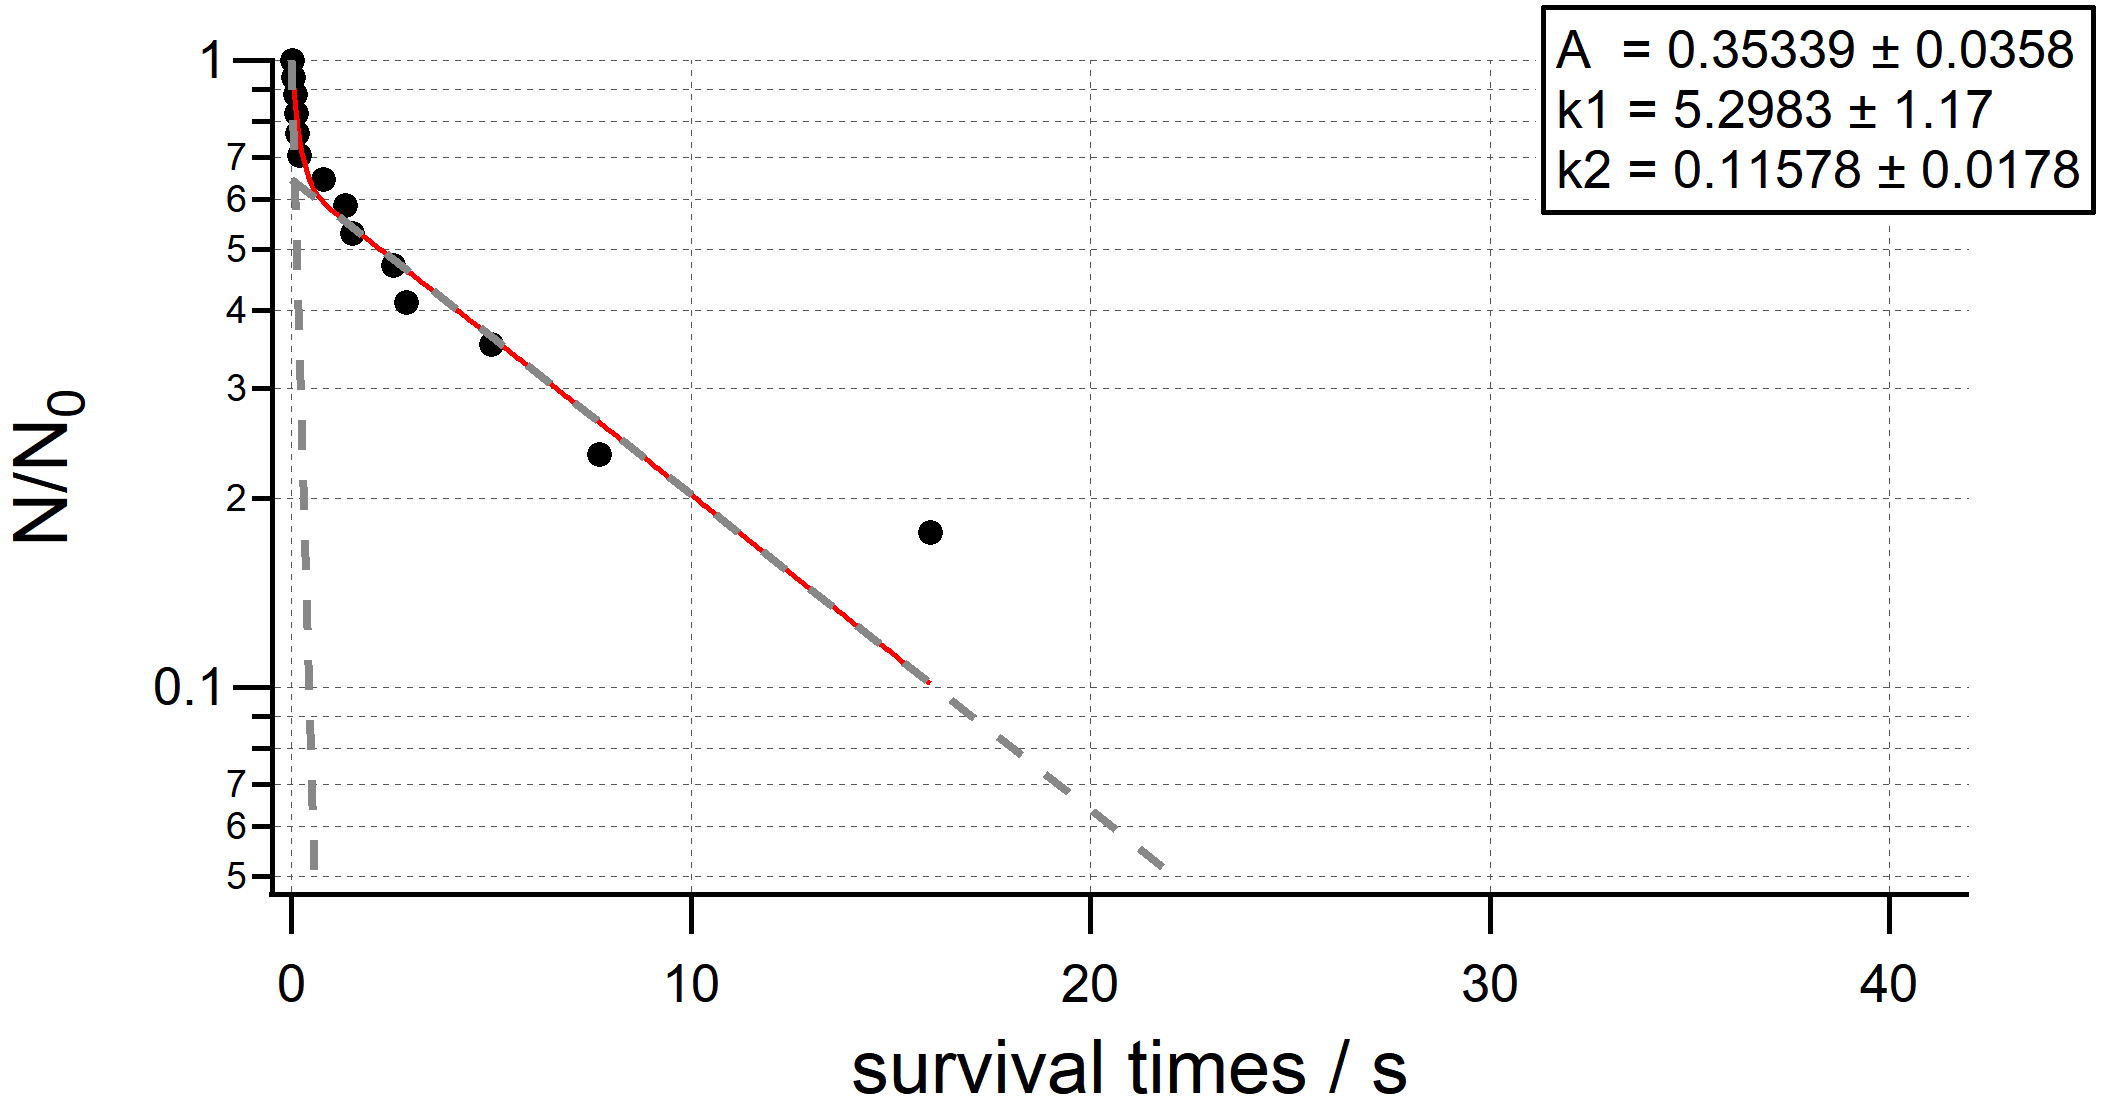
\includegraphics[width=\linewidth]{Abbildungen/clamp_ph_8_multiple_ruptures.png}
	} % scalebox
	\caption[Ergebnisse der Force-Clamp-Experimente bei einem pH-Wert von 8]{Ergebnisse der Force-Clamp-Experimente bei einem pH-Wert von 8. Es konnten zwei Zerfallsprozesse beobachtet werden. Die Geschwindigkeitskonstante (grau gestrichelte Linien) $k_1~=~5,3~s^{-1}~\pm~1,84~s^{-1}$ und $k_2~=~0,12~s^{-1}~\pm~0,018~s^{-1}$, sowie der Mischungskoeffizient beider Prozesse $A~=~0,35~\pm~0,036$ konnten durch die Anpassung eines biexponentiellen Zerfalls an die Daten ermittelt werden. Für diese Auswertung wurden insgesamt 14 Clampereignisse verwendet.}
	\label{fig:clamp_8}
\end{figure}


% Ergebnisse Clamp pH7,4
\begin{figure}[H]
	\centering
	\scalebox{0.9}{
		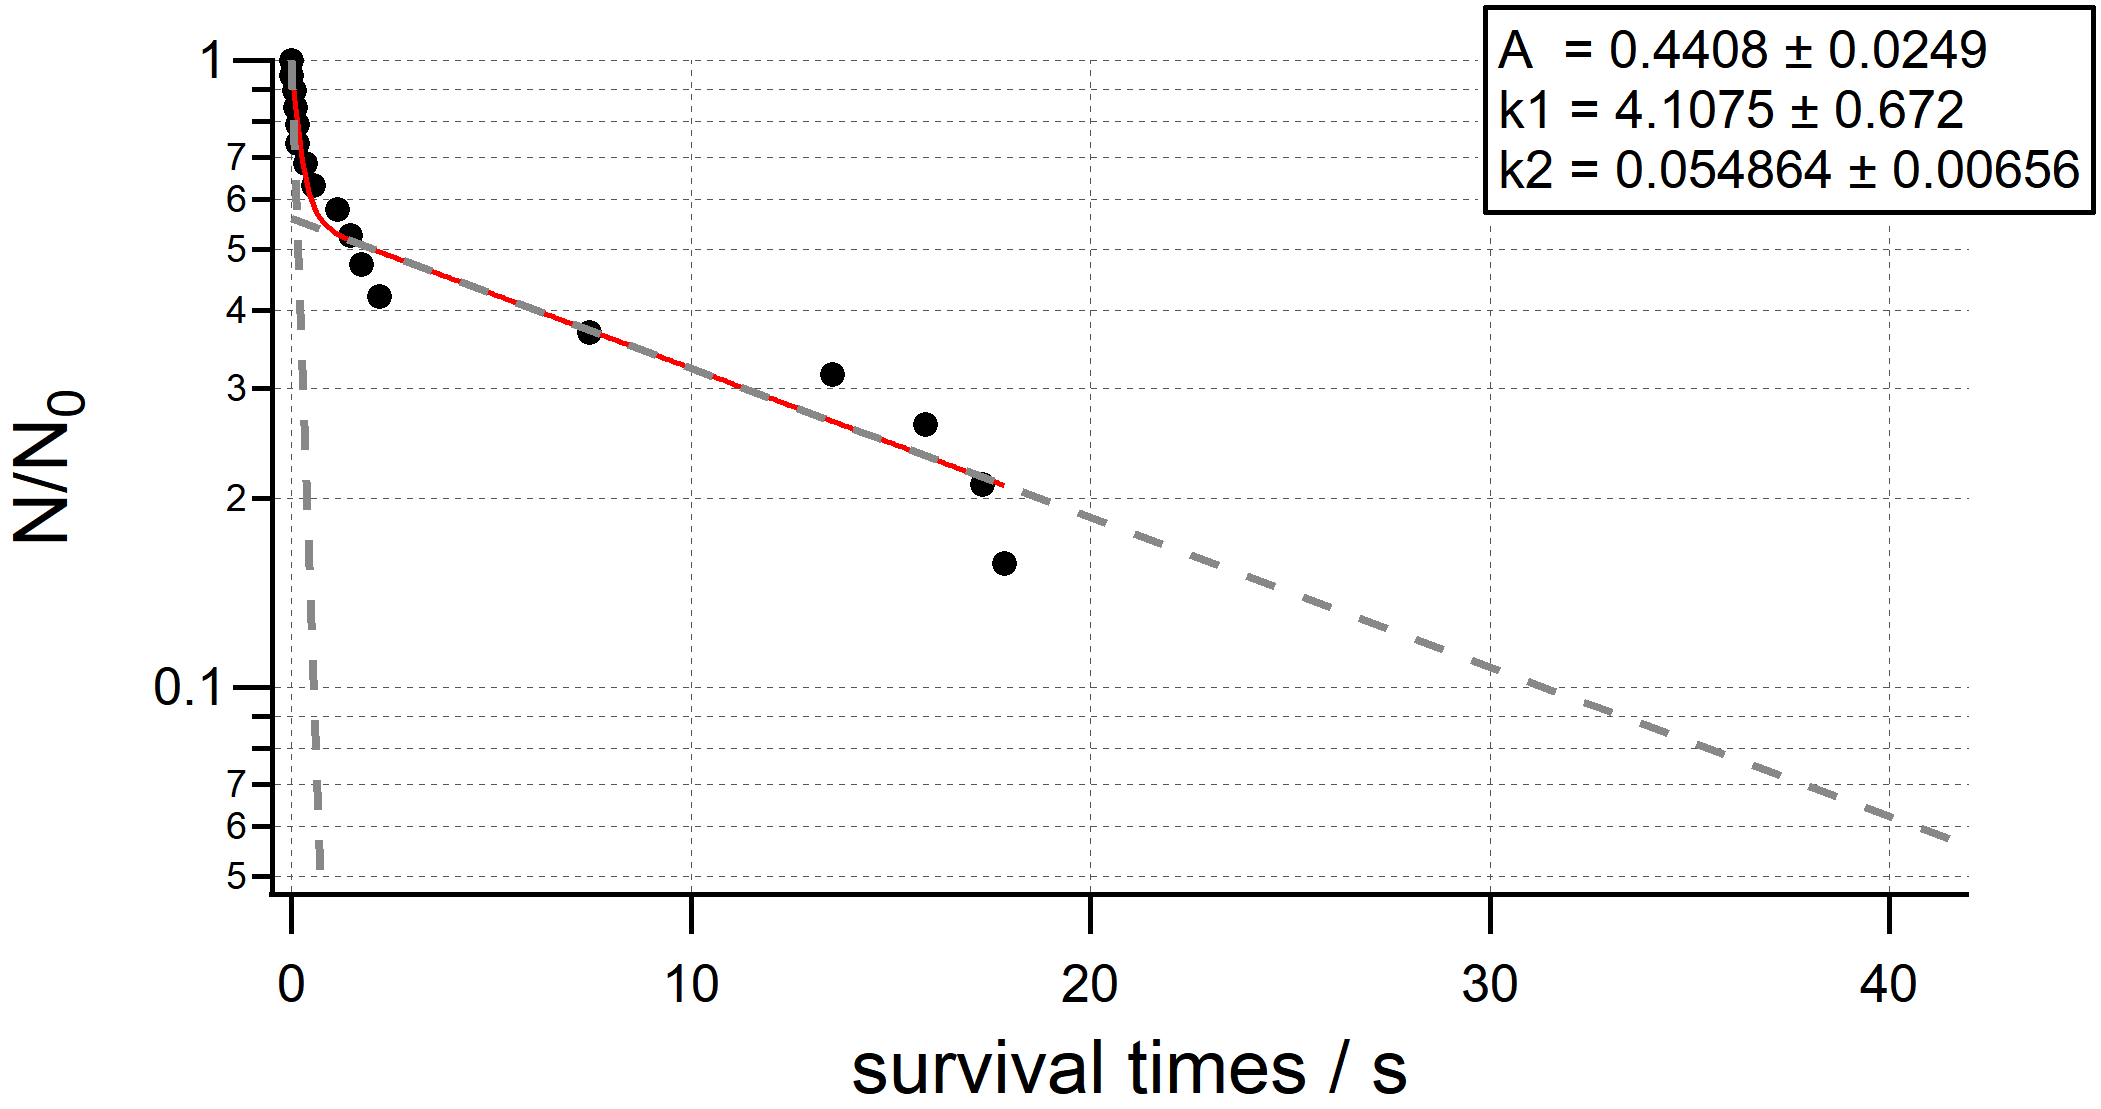
\includegraphics[width=\linewidth]{Abbildungen/clamp_ph7_4_multiple_ruptures.png}
	} % scalebox
	\caption[Ergebnisse der Force-Clamp-Versuche bei einem pH-Wert von 7,4]{Ergebnisse der Force-Clamp-Versuche bei einem pH-Wert von 7,4.  Es konnten zwei Zerfallsprozesse beobachtet werden. Die Geschwindigkeitskonstante (grau gestrichelte Linien) $k_1~=~4,1~s^{-1}~\pm~0,67~s^{-1}$ und $k_2~=~0,055~s^{-1}~\pm~0,0066~s^{-1}$, sowie der Mischungskoeffizient beider Prozesse $A~=~0,44~\pm~0,025$ konnten durch die Anpassung eines biexponentiellen Zerfalls an die Daten ermittelt werden. Für diese Auswertung wurden insgesamt 16 Clampereignisse verwendet.}
	\label{fig:clamp_7_4}
\end{figure}

% Ergebnisse Clamp pH4,5
\begin{figure}[H]
	\centering
	\scalebox{0.9}{
		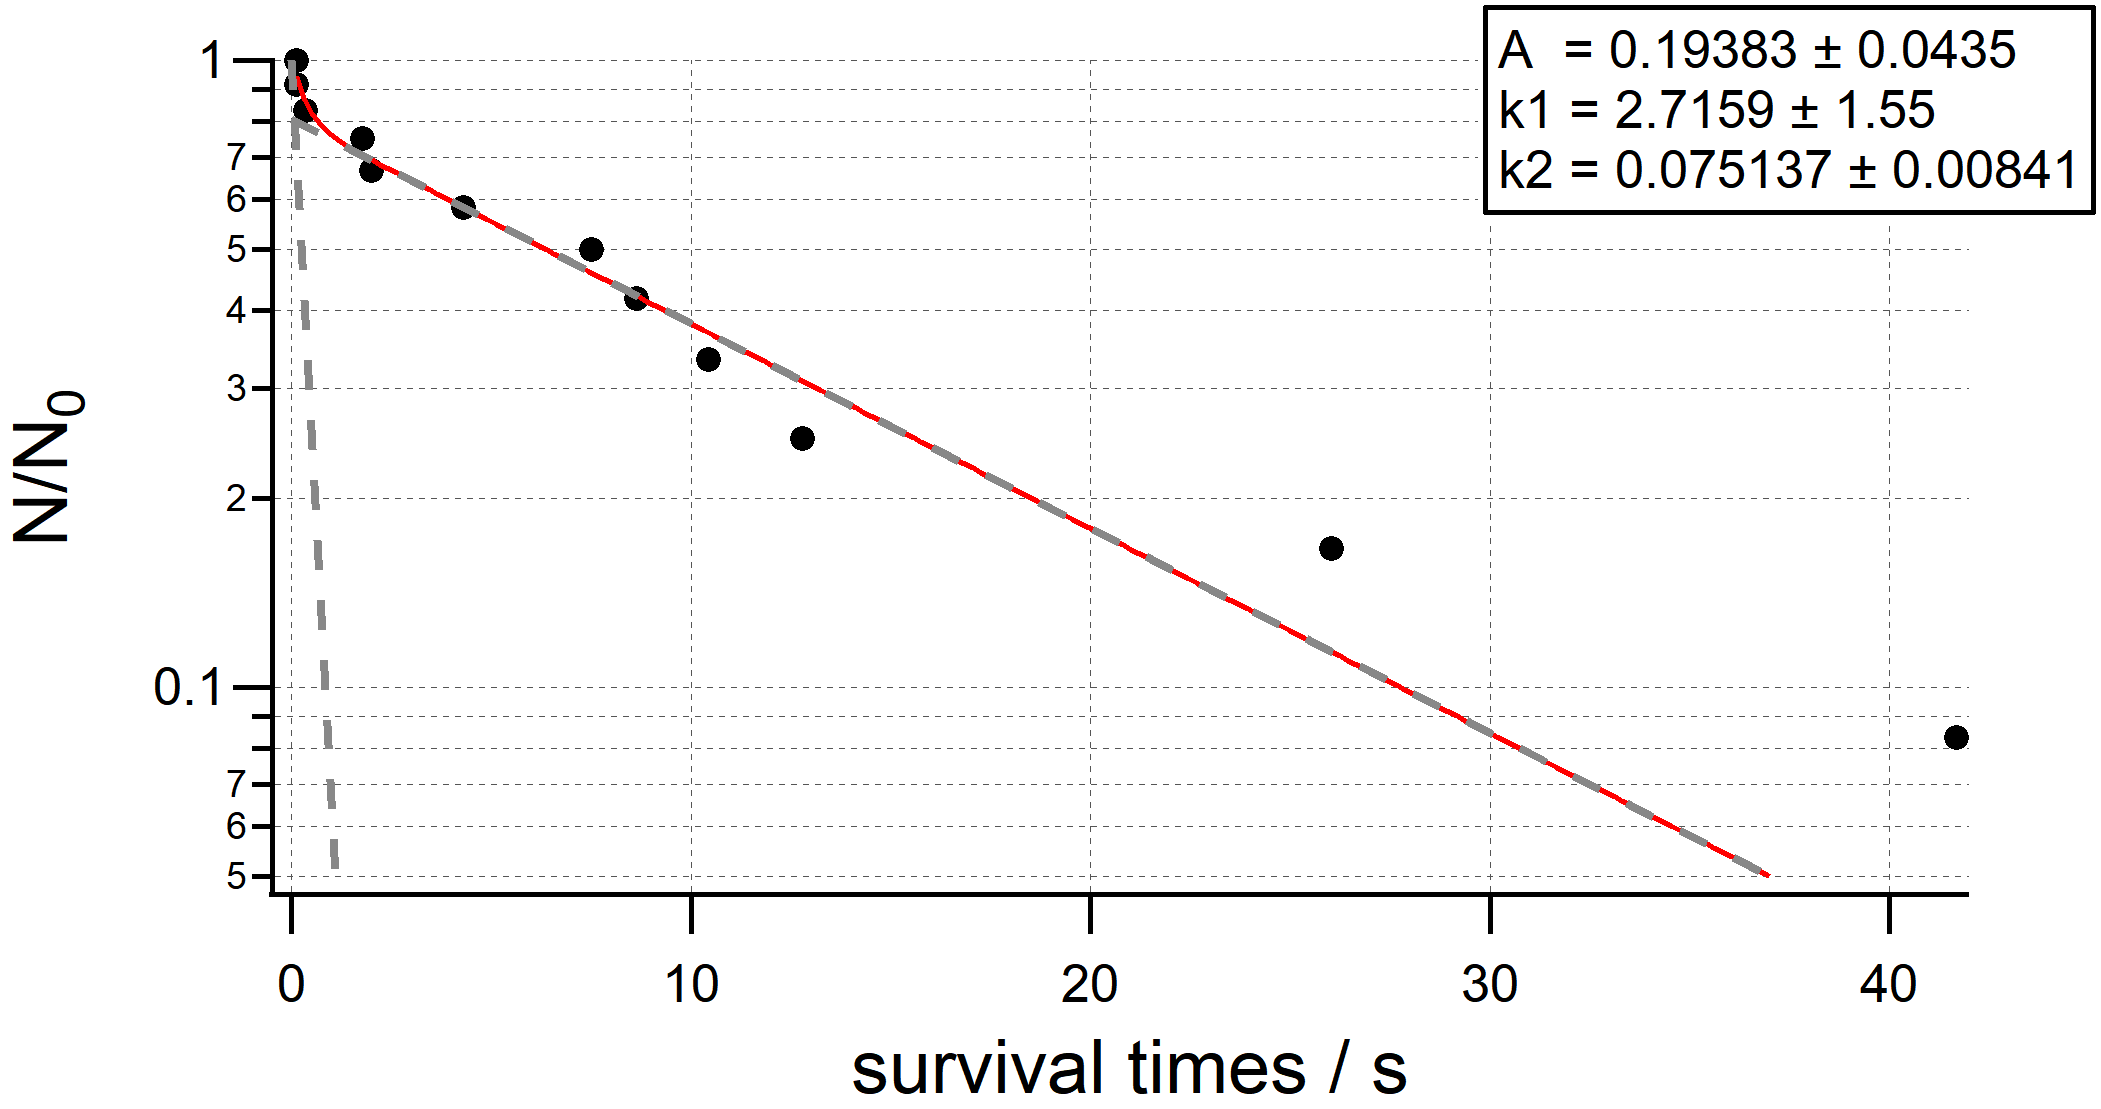
\includegraphics[width=\linewidth]{Abbildungen/clamp_ph4_5_multiple_ruptures.png}
	} % scalebox
	\caption[Ergebnisse der Force-Clamp-Versuche bei einem pH-Wert von 4,5]{Ergebnisse der Force-Clamp-Versuche bei einem pH-Wert von 4,5. Es konnten zwei Zerfallsprozesse beobachtet werden. Die Geschwindigkeitskonstante (grau gestrichelte Linien) $k_1~=~2,7~s^{-1}~\pm~1,55~s^{-1}$ und $k_2~=~0,075~s^{-1}~\pm~0,0084~s^{-1}$, sowie der Mischungskoeffizient beider Prozesse $A~=~0,19~\pm~0,044$ konnten durch die Anpassung eines biexponentiellen Zerfalls an die Daten ermittelt werden. Für diese Auswertung wurden insgesamt 11 Clampereignisse verwendet.}
	\label{fig:clamp_4_5}
\end{figure}

In \abb~\ref{fig:general_curve_composition} wurde die kategorische Zusammensetzung aller aufgenommenen Kraftkurven der jeweiligen pH-Werte aufgeschlüsselt. Zur Auswertung wurden ausschließlich Kraftkurven aus den Kategorien A und B, ohne zusätzliche Bemerkungen herangezogen. Diese beiden Kategorien stellten die Ausbeute der Force-Clamp-Experimente dar (grüne und blaue Bereiche in \abb~\ref{fig:general_curve_composition}). Die Ausbeute ergab 9\% für pH 8, 5\% für pH 7,4 und 29\% für pH 4,5. Tabelle~\ref{tab:general_curve_composition} verdeutlicht diesen Sachverhalt. Das Verhältnis von Kategorie A zu Kategorie B Kurven kurz $A/B$, lag für pH 4,5 bei 0,32. Im Vergleich zu den anderen pH-Werten ($A/B^{7,4} = 4$ bzw. $A/B^{8} = 1,25$) sehr weit unterhalb von 1. Für die Auswertung der Force-Clamp-Experimente bei pH 4,5 standen demnach hauptsächlich Kategorie B kurven zur Verfügung. Bei den pH-Werten 8 und 7,4 hingegen standen hauptsächlich Kategorie A zur Verfügung. Das vermehrte Auftreten von Kategorie B Kurven bei dem pH-Wert von 4,5 verglichen mit den pH-Werten von 8 und 7,4 deutete auf eine höhere Interaktion zwischen \spitze~dem \spacer~und dem Substrat hin.

% General Curve Composition
\begin{figure}[H]
	\centering
	\scalebox{0.9}{
		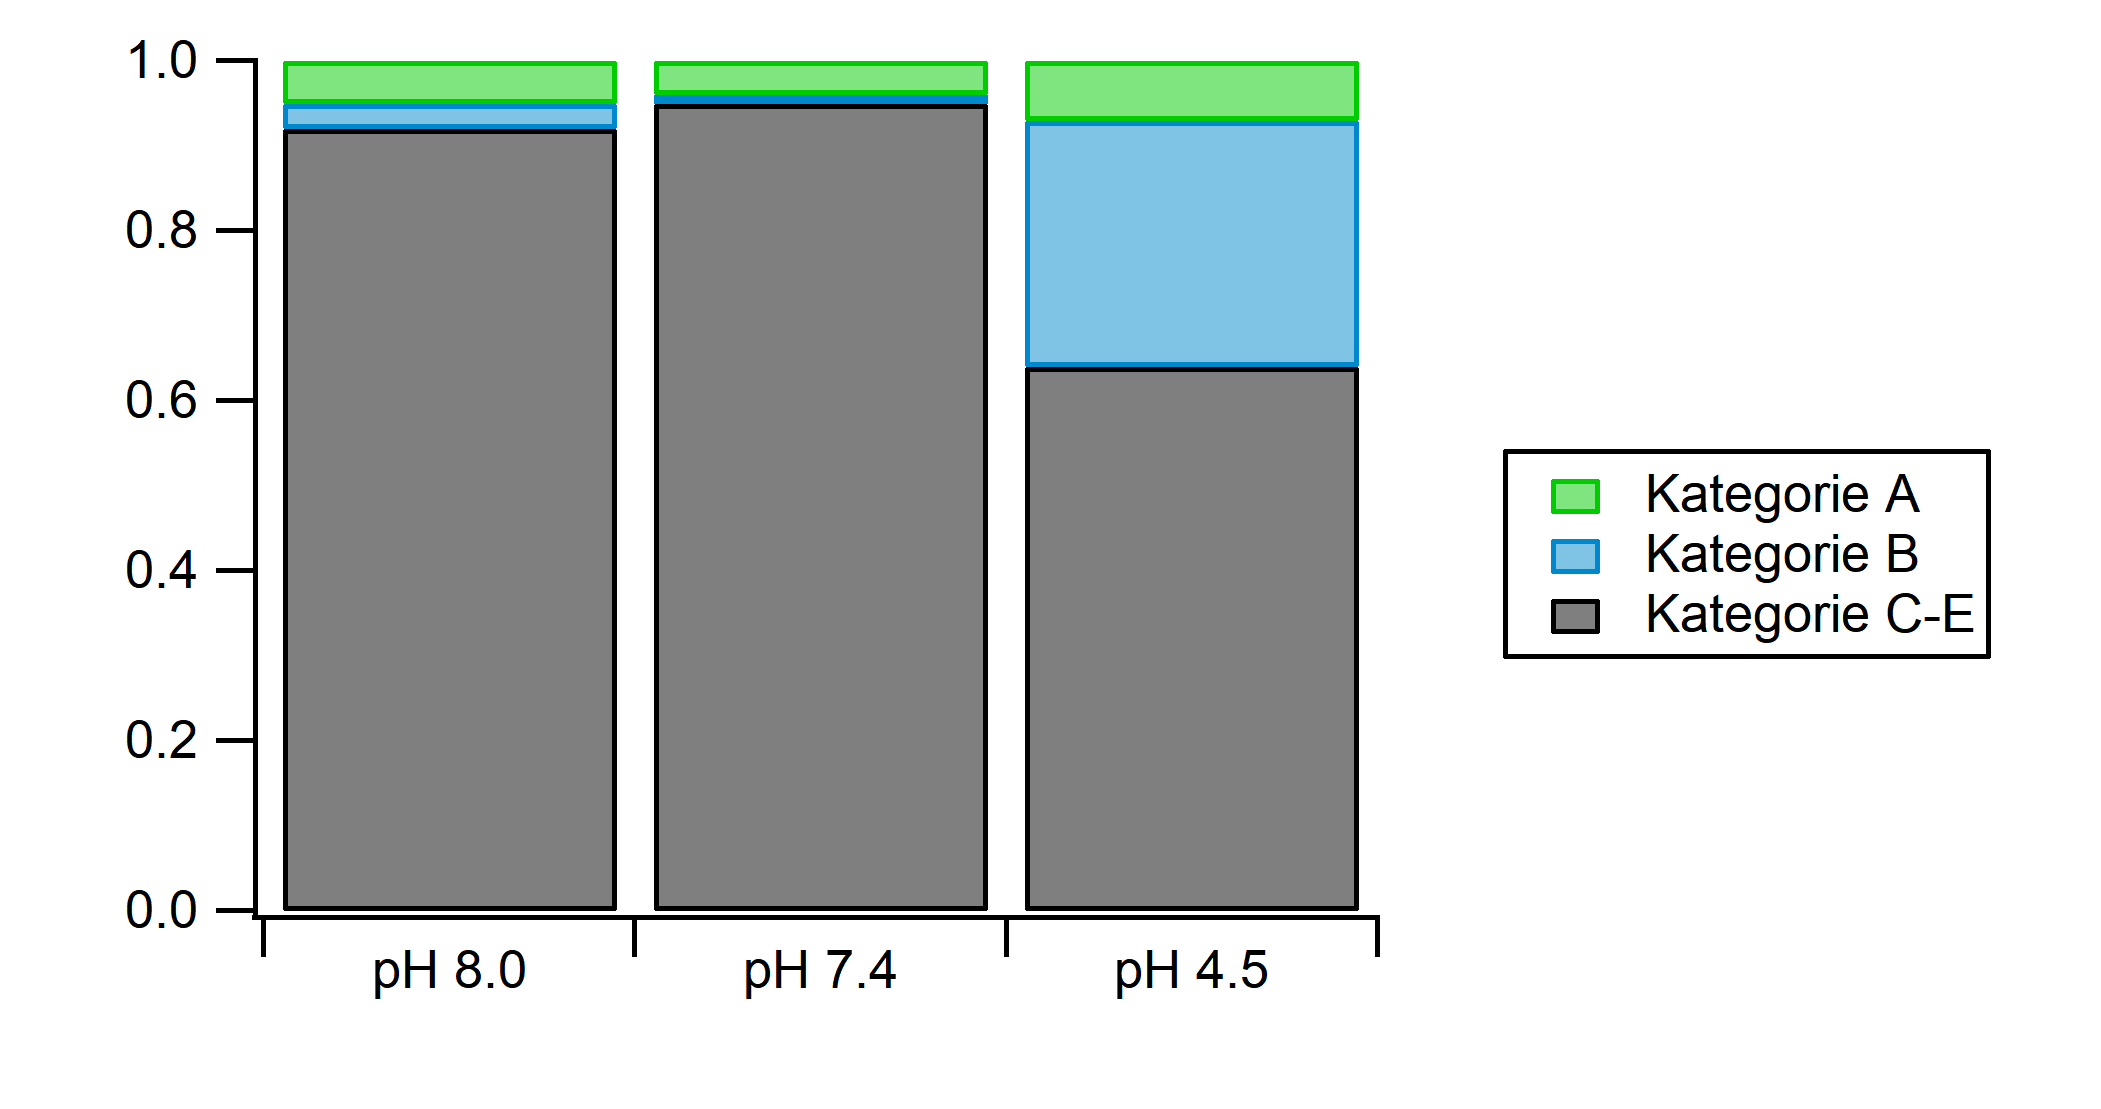
\includegraphics[width=\linewidth]{Abbildungen/curve_composition_multiple_ruptures.png}
	} % scalebox
	\caption[Kategorische Zusammensetzung aller aufgenommenen Kraftkurven]{Kategorische Zusammensetzung aller aufgenommenen Kraftkurven der Experimente bei den pH-Werten 8, 7,4 und 4,5. Kategorie A (pH = 8): 5\%. Kategorie B (pH = 8): 3\%. Kategorie C-E (pH = 8): 91\%. Kategorie A (pH = 7,4): 4\%. Kategorie B (pH = 7,4): 1\%. Kategorie C-E (pH = 7,4): 95\%. Kategorie A (pH = 4,5): 7\%. Kategorie B (pH = 4,5): 29\%. Kategorie C-E (pH = 4,5): 64\%. $N_8$ = 155, $N_{7,4}$ = 360, $N_{4,5}$ = 41.}
	\label{fig:general_curve_composition}
\end{figure}

% Zusammensetzung und Ausbeute der Force-Clamp-Experimente
\begin{table}[H]
	\centering
	\caption[Kategorische Zusammensetzung aller ausgewerteten Clampereignisse]{Kategorische Zusammensetzung aller ausgewerteten Clampereignisse bei unterschiedlichen pH-Werten.}
	\label{tab:general_curve_composition}
	\begin{threeparttable}
		\keepXColumns
		\begin{tabularx}{\textwidth}{X X X X}
			\textbf{pH-Wert}	&	\textbf{Kategorie A /\%}	&	\textbf{Kategorie B /\%}	&	\textbf{Kategorie C-E/\%}	\\
			\toprule
			\toprule
			8	&	5	&	4	&	91	\\
			7,4	&	4	&	1	&	95	\\
			4,5	&	7	&	22	&	71	\\
			\toprule
			\toprule
		\end{tabularx}
	\end{threeparttable}
\end{table}

Ein ähnliches Bild ergab sich bei den verworfenen Kraftkurven (Kategorie C-E). In \abb~\ref{fig:discarded_curve_composition} wurden ausschließlich die verworfenen Kraftkurve bei den verschiedenen pH-Werten nach Kategorien aufgeschlüsselt. Kraftkurven aus den Kategorien C und D konnten keiner Einzelmolekülinteraktion zugeordnet werden, zeigten jedoch deutliche Mehrfach- oder überlagerte Mehrfachabrisse. Kraftkurven der Kategorie E zeigten keinerlei molekülspezifische Interaktionen zwischen Substrat und \spitze~(s. Abschnitt~\ref{subsec:kategorisierung_der_kraftkurven}). Tabelle~\ref{tab:discarded_curve_composition} fast die kategorische Aufschlüsselung aus \abb~\ref{fig:discarded_curve_composition} Zusammen. Kategorie C Kurven erschienen ausschließlich bei pH 8 und wurden nicht weiter berücksichtigt. Die Zusammensetzung der verworfenen Kraftkurven zeigte eine Zunahme von Kategorie D Kurven bei pH 4,5. Das Verhältnis von Kategorie C zu D Kurven lag bei pH 4,5 ($C/D^{4,5} = 0,69$) mehr als doppelt so hoch wie bei den anderen pH-Werten ($C/D^{8} = 0,33$ und $C/D^{7,4} = 0,25$). Dies passte zur Aussage von \abb~\ref{fig:general_curve_composition}, denn auch in den verworfenen Kraftkurven zeigte sich bei pH 4,5 eine erhöhte Interaktion.

% Discarded Curve Composition
\begin{figure}[H]
	\centering
	\scalebox{0.9}{
		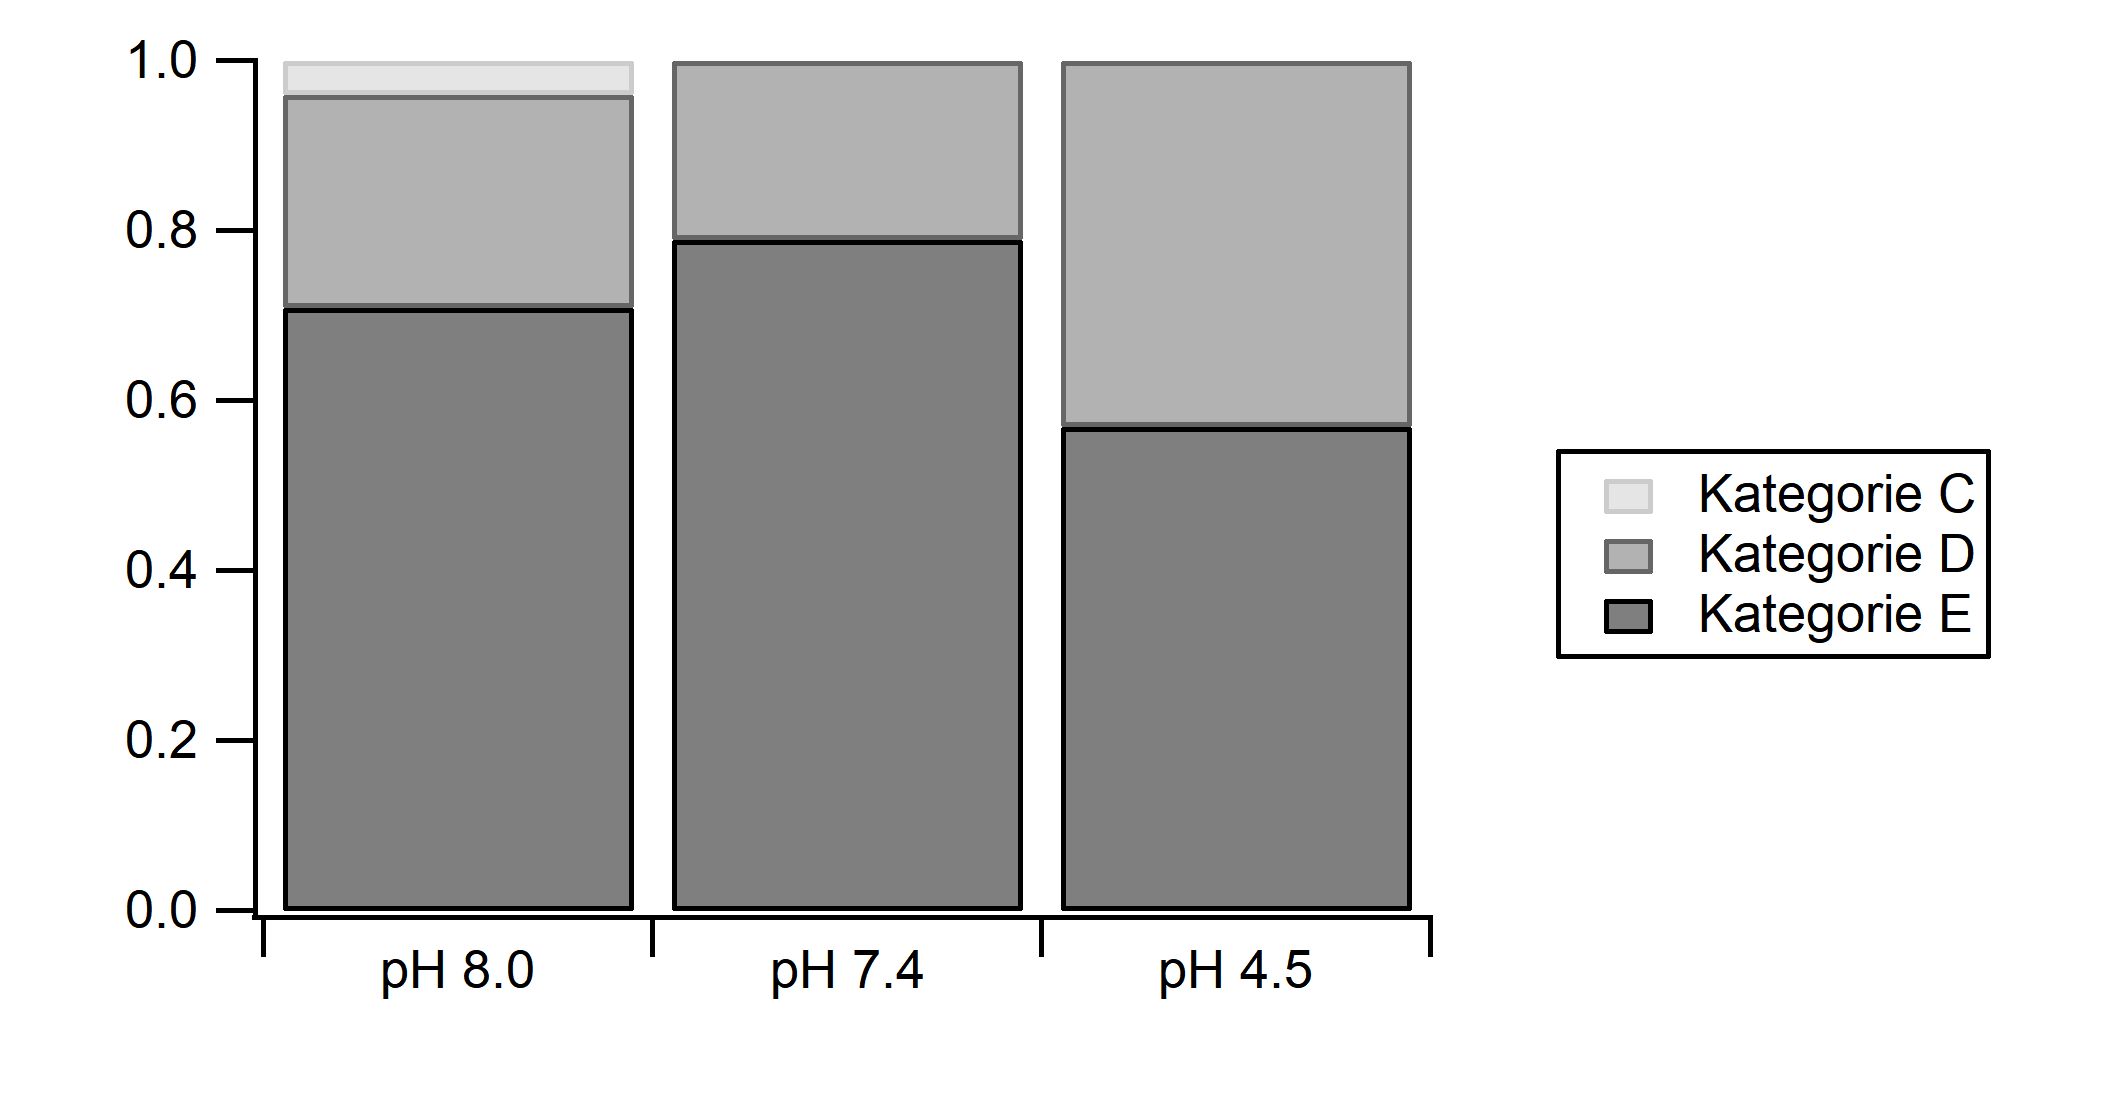
\includegraphics[width=\linewidth]{Abbildungen/discarded_curve_composition_multiple_ruptures.png}
	} % scalebox
	\caption[Kategorische Zusammensetzung aller verworfenen Kraftkurven]{Kategorische Zusammensetzung aller verworfenen Kraftkurven der Experimente bei den pH-Werten 8, 7,4 und 4,5. Kategorie C (pH = 8): 4\%. Kategorie D (pH = 8): 25\%. Kategorie E (pH = 8): 71\%. Kategorie C (pH = 7,4): 0\%. Kategorie D (pH = 7,4): 21\%. Kategorie E (pH 0 7,4): 79\%. Kategorie C (pH = 4,5): 0\%. Kategorie D (pH = 4,5): 43\%. Kategorie E (pH = 4,5): 57\%. $N_8$ = 139, $N_{7,4}$ = 332, $N_{4,5}$ = 28.}
	\label{fig:discarded_curve_composition}
\end{figure}

% Kategoriesche Zusammensetzung der verworfenen Kraftkurven
\begin{table}[H]
	\centering
	\caption[Kategorische Zusammensetzung aller verworfener Clampereignisse]{Kategorische Zusammensetzung aller verworfenen Clampereignisse bei unterschiedlichen pH-Werten.}
	\label{tab:discarded_curve_composition}
	\begin{threeparttable}
		\keepXColumns
		\begin{tabularx}{\textwidth}{X X X X}
			\textbf{pH-Wert}	&	\textbf{Kategorie C /\%}	&	\textbf{Kategorie D /\%}	&	\textbf{Kategorie E/\%}	\\
			\toprule
			\toprule
			8	&	4	&	25	&	71	\\
			7,4	&	0	&	21	&	79	\\
			4,5	&	0	&	43	&	57	\\
			\toprule
			\toprule
		\end{tabularx}
	\end{threeparttable}
\end{table}
	\chapter{Diskussion}
\label{kap:diskussion}

Die Auswertungen der experimentellen Daten durch einen Biexponentiellen Zerfall lieferte robuste Parameterschätzungen (für $k_1$, $k_2$ und $A$), wenn ausreichend Datenpunkte für den schnellen und langsamen Prozess vorhanden waren und $A \approx 0,5$. Robust bedeutet, dass die Fehler der Fitparameter mindestens eine Größenordnung kleiner sind als der Wert des Fitparameters selbst. In den Force-Clamp-Experimenten bei den pH-Werten 8, 7,4 und 4,5 erfüllte ausschließlich das Force-Clamp-Experiment bei pH 7,4 diese Kriterien. Bei pH 8 fielen nur 5 Datenpunkte in den schnellen Prozess, sodass $\Delta k_1^{8}  \approx k_1^{8}$. Bei pH 4,5 war nicht mit Sicherheit zu sagen ob ein schneller Prozess vorhanden war, da nur 2 Datenpunkte in diesen Prozess vielen.\\
Interessant ist jedoch generell das Auftreten eines schnellen und eines langsamen Prozesses. Es stellen sich daher die Fragen:

\begin{itemize}
	\item Welcher Prozess stellt die Hydrolyse der \amid~ dar?
	\item Was bedeutet der andere Prozess?
\end{itemize}

Um zu zeigen, dass die \amid~ in der Kette zwischen Substrat, \spacer~ und \spitze~ das schwächste Glied war, wurden in einer anderer Arbeit folgende Kontrollen durchgeführt~\cite{ClausenSchaumann.2018}:

\begin{itemize}
	\item Austausch der \aminos~auf Substrat und \spitze~durch \carboxys~(Bildung von Esterbindungen zwischen \ac{CMA} und Substrat/ \spitze)
	\item Austausch von \ac{CMA} durch Biscarboxy-PEG bzw. Adipinsäure (keine glykosidischen Bindungen innerhalb des \spacers)
\end{itemize}

%%% Fußnotentext
\renewcommand{\noteOne}{Die Dissoziationsenergie der O-O-Bindung liegt bei $142~kJ~mol^{-1}$. Verglichen mit einer C-C-Bindung mit $339~kJ~mol^{-1}$ oder C-O-Bindung mit $331~kJ~mol^{-1}$ um mehr als die Hälfte schwächer \cite[15]{Latscha.2016}}
%%% Endefußnotentext


Wurde in einem Force-Clamp-Experiment an einer Esterbindung gemessen, lag $\tau$ bei ca. 4 Sekunden. Wurde der \spacer~durch Biscarboxy-PEG oder Adipinsäure ersetzt und an der Amidbindung gemessen lag $\tau$ bei ca. 0,17 Sekunden. All diese Experimente wurden bei pH = 7,4 durchgeführt. Ein Vergleich von \cite{ClausenSchaumann.2018} und den hier durchgeführten Force-Clamp-Experimenten lässt vermuten, dass es sich bei dem schnellen Prozess um die Hydrolyse der \amid~handelte. Demnach konnte es sich bei dem langsamen Prozess nicht um die Beeinflussung der \amid~durch den Einbau von \ch{O2} während der Funktionalisierung des Substrats/ \spitze~handeln (s. Abschnitt~\ref{subsec:oberflächenfunktionalisierung_via_kohlenstoffanker}). Wird davon ausgegangen, dass sich Peroxidbrücken gebildet hätten, wäre die Wahrscheinlichkeit hoch, dass diese während der Oberflächenfunktionalisierung unter UV-Lichteinwirkung (λ= 254 nm) homolytisch gespalten worden wären\footnote{\noteOne}. Prinzipiell wären dann folgende Reaktionen möglich: 


\begin{eqnarray}
	\ch[arrow-min-length=2cm]{S-O-O-R1	&	->[$h\nu$]	&	S-O. + .O-R1} \label{scheme:peroxid_step_1}\\
	\ch[arrow-min-length=2cm]{S-O. + R2 + H.	&	->	&	S-O-R2H} \label{scheme:peroxid_step_2}\\
	\ch[arrow-min-length=2cm]{S-O. + H.	&	->	&	S-OH} \label{scheme:peroxid_step_3}\\
	\ch[arrow-min-length=2cm]{R3 + .O-R1 + H.	&	->	&	HR3-O-R1} \label{scheme:peroxid_step_4}\\
	\ch[arrow-min-length=2cm]{H. + .O-R1	&	->	&	HO-R1} \label{scheme:peroxid_step_5}
\end{eqnarray}

Wobei $R_1$, $R_2$ und $R_3$ jeweils für unterschiedliche Allylamin-Moleküle und $S$ für das Substrat (wahlweise auch für die \spitze) stehen. Hier wurde das baumartige Wachstum von Allylamin auf dem Substrat bzw. der Abtastspitze nicht berücksichtigt. Unter der Annahme, dass sich die Peroxidbrücken (Reaktion~\ref{scheme:peroxid_step_1}) gespalten hätten, wäre die Wahrscheinlichkeit dafür, dass die Peroxide im Laufe der Funktionalisierung zu Ethern reagierten (Reaktion~\ref{scheme:peroxid_step_2}) sehr hoch (vgl.~\cite[15]{Latscha.2016}). Die Reaktionen~\ref{scheme:peroxid_step_3}~bis~\ref{scheme:peroxid_step_5} würden die Ausbeute der Funktionalisierung herabgesetzten und die Ausbildung einer \amid~verhindern. Die Etherbrücken, gebildet nach Reaktion~\ref{scheme:peroxid_step_2}, waren unter Krafteinfluss jedoch stabiler als die \amid~(vgl.~\cite{ClausenSchaumann.2018}) und wären damit nicht in den durchgeführten Force-Clamp-Experimenten sichtbar gewesen. Dabei wird davon ausgegangen, dass sich der Sauerstoff zwischen Substrat und der \amid~befindet und somit an Ether und an Amid gleichzeitig gemessen wurde. Auch die Bildung von Estern, statt der Amide, durch die Einführung von Hydroxylgruppen auf dem Substrat bzw. der \spitze~wie in Reaktion~\ref{scheme:peroxid_step_3} gezeigt ist, wäre möglich, jedoch entspricht keine der hier ermittelten mittleren Lebensdauern der langsamen Prozesse der des Esters ($\tau_{Ester}  = 4~s$) aus \cite{ClausenSchaumann.2018}.\\

Weitere Ursachen, die den langsamen Prozess hervorrufen:

\begin{itemize}
	\item Das Auftreten einer zweiten Bindungsart
	\item Beeinflussung der Amidhydrolyse
	\item Mehrfach, parallel gebildete \amide~zwischen den \carboxys~eines einzigen \spacer~an Substrat und \spitze
\end{itemize}

%% Fußnotentext
\renewcommand{\noteOne}{Abgesehen von Hydroxylgruppen. Die daraus resultierenden Ester konnten anhand ihrer mittleren Lebensdauer für den langsamen Prozess ausgeschlossen werden (s.o.).}

\renewcommand{\noteTwo}{Die nukleophile Addition von \ch{H2O} an das Carbonylkohlenstoff ist die initiale Reaktion für die Hydrolyse. Diese Reaktion kann durch Säuren oder Basen beschleunigt werden 	\cite[288]{Latscha.2016}}

\renewcommand{\noteThree}{Die Reaktivität der Carbonsäurederivate beruht auf der Basizität des Substituenten. Je geringer die Basizität, desto stabiler ist das Derivat. Die Einteilung nach steigender Reaktivität lautet dabei wie folgt \cite[287]{Latscha.2016}:
	\scalebox{0.9}{
		\setchemfig{scheme debug = false}
		\setchemfig{angle increment=30}
		\definesubmol{rest}{R-[,0.75]C(=[2,0.75]O)-[-2,0.75]}
		\schemestart
		\chemname{
			\chemfig{!{rest}OH}
		}{Carbonsäure}
		\arrow(.base east--.base west){0}[,0]<\arrow(.base east--.base west){0}[,0.3]
		\chemname{
			\chemfig{!{rest}NH_2}
		}{-amid}
		\arrow(.base east--.base west){0}[,0]<\arrow(.base east--.base west){0}[,0.3]
		\chemname{
			\chemfig{!{rest}OR}
		}{-ester}
		\arrow(.base east--.base west){0}[,0]<\arrow(.base east--.base west){0}[,0.3]
		\chemname{
			\chemfig{!{rest}SR}
		}{-thioester}
		\arrow(.base east--.base west){0}[,0]<\arrow(.base east--.base west){0}[,0.3]
		\chemname{
			\chemfig{R-[,0.75]C(=[2,0.75]O)-[-1,0.75]O-[1,0.75]C(=[4,0.75]O)-[,0.75]R}
		}{-anhydrid}
		\arrow(.base east--.base west){0}[,0.3]<\arrow(.base east--.base west){0}[,0.3]
		\chemname{
			\chemfig{!{rest}Cl}
		}{-chlorid}
		\schemestop
	}
}
%%% Ende Fußnotentext

Der langsame Prozess könnte über eine zweite Bindungsart erklärt werden, wenn angenommen wird, dass die Oberflächen von Substrat und \spitzen~mit anderen funktionellen Gruppen ausgestattet worden wären\footnote{\noteOne}, oder ein Tausch der funktionellen Gruppen stattgefunden hätte. Für beides wären jedoch spezielle Substanzen nötig, die nicht zufällig durch unsauberes Arbeiten eingebracht werden konnten. Das Auftreten einer zweiten Bindungsart kann daher ausgeschlossen werden.\\

Es bleibt bisher ungeklärt, welche Reaktionen generell an sekundären Carbonsäureamiden ablaufen können. Die Frage ist wie sich etwaige Verunreinigungen oder Reaktionsnebenprodukte auf die \amid~auswirkten. Die typische Angriffspunkte der Carbonsäureamide sind die Carbonylgruppe (\abb~\ref{fig:amidbindung}, Position~1) und das C-Atom in $\alpha$-Stellung zur Carbonylgruppe (\abb~\ref{fig:amidbindung}, Position~2). An diesen Stellen wären eine Reihe von Reaktionen möglich \cite[305-308]{Latscha.2016}. An der Carbonylgruppe könnten in erster Linie Additionsreaktionen (sowohl nukleophil\footnote{\noteTwo} durch den Angriff am Carbonylkohlenstoff oder elektrophil durch den Angriff an der Doppelbindung der Carbonylgruppe) durchgeführt werden. Daneben könnte die Carbonylgruppe reduziert, bzw. oxidiert werden. Das Kohlenstoffatom in $\alpha$-Stellung könnte deprotoniert werden und so das Carbonsäureamid in seine Enolatform überführt werden. An der entstandenen Doppelbindung zum $\alpha$-C-Atom können wiederum elektrophile Additionsreaktionen durchgeführt werden. Da Carbonsäureamide zu den schwach reaktiven Carbonsäurederivaten\footnote{\noteThree} zählt, sind für die oben genannten Reaktionen jedoch starke Reagenzien notwendig. Reaktionen am Stickstoffatom finden nicht statt. Zum einen war die Basizität durch eine Keto-Enol-Tautomerie der C-N-Bindung und zum anderen die N-H-Acidität durch +I-Effekte der Substituenten am Stickstoffatom herabgesetzt. 

% Reaktionspositionen der Amidbindung
\begin{figure}[h]
	\centering
	\scalebox{0.5}{
		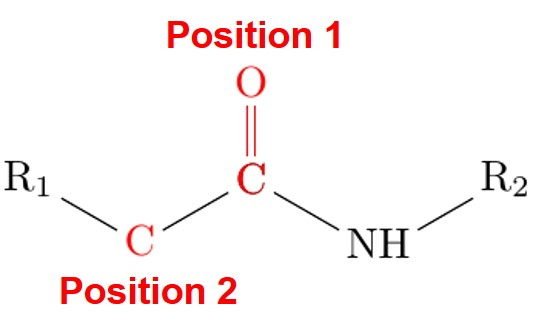
\includegraphics[width=\linewidth]{Abbildungen/amide_bond_II.jpg}
	} % scalebox
	\caption[Amidbindung eines Carbonsäureamids]{Amidbindung eines Carbonsäureamids. Position~1: Carbonylgruppe. Position~2: C-Atom in $\alpha$-Stellung zur Carbonylgruppe. $R_1$ steht für den Allylaminrest an Substrat/ \spitze, $R_2$ für die Fortsetzung des \acs*{CMA}-Spacers.}
	\label{fig:amidbindung}
\end{figure}

Eventuelle Verunreinigungen oder Reaktionsnebenprodukte der einzelnen Funktionalisierungen können sich entweder auf die Kinetik, oder den Mechanismus der Amidhydrolyse auswirken. Die Kinetik ändert sich, wenn die Aktivierungsenergien der \ac{UZ} geändert werden, oder der Übergang von \ac{TZP} zu \ac{ZI} erleichtert bzw. behindert wird.\\
Für eine Änderung des Reaktionsmechanismus muss die Struktur der Amidbindung durch chemische Reaktionen geändert werden.\\

Die Beeinflussung der Hydrolyse durch Reaktionsnebenprodukte kann jedoch ausgeschlossen werden, da sie durch die jeweiligen Waschschritte entfernt worden sind. Quellen für sonstige Verunreinigungen sind vor allem organische Rückstände (hauptsächlich Fette) oder Mineralablagerungen (\ch{CaCO3} und \ch{MgCO3}) auf den Oberflächen der verwendeten Petrischalen und Pinzetten. Da organische Ablagerungen in Form von Fetten unlöslich sind, würden sie als Oberflächenfilm auf die Substrate übertragen und die Bildung von \amide~an diesen Stellen verhindern. Mineralablagerungen sind in wässrigen Medien schwer löslich und kommen in äußerst geringen Mengen vor (maximal $1~mg$). Verglichen mit dem Volumen der \ac{PBS}-Lösungen in den verwendeten Petrischalen (ca. $5~ml$) wäre die Konzentration von \ch{CaCO3} bzw. \ch{MgCO3} mit $c \approx 2~mmol~l^{-1}$ sehr nahe bei null. Mögliche Änderungen des pH-Wertes, sowie ionische Einflüsse von \ch{Ca^2+}- bzw. \ch{Mg^2+}-Ionen sind damit Vernachlässigbar.\\
Eventuelle ionische Effekte auf die Kinetik der Amidhydrolyse würden sich auf alle Experimente (hier durchgeführte Force-Clamp-Experimente, sowie die Kontrollen in \cite{ClausenSchaumann.2018}) gleichermaßen auswirken und die Hydrolysereaktion entweder beschleunigen, oder verlangsamen, jedoch nicht beides zur gleichen Zeit.\\

Um die Struktur der Amidbindung zu ändern, sind zwei Reaktionen von Bedeutung~\cite[301\psqq]{Latscha.2016}: 

\begin{itemize}
	\item Reduktion der Carbonylgruppe (Position 1, \abb~\ref{fig:amidbindung})
	\item Deprotonierung des $\alpha$-C-Atoms (Position 2, \abb~\ref{fig:amidbindung})
\end{itemize} 

Für die Reduktion der Carbonylgruppe sind jedoch starke Reduktionsmittel wie \ch{LiAlH4} notwendig \cites[306]{Latscha.2016}[208]{Leisering.2017}. Es ist sehr unwahrscheinlich, dass solche Verbindungen als Verunreinigung von außen eingetragen wurden. Die Deprotonierung des $\alpha$-C-Atoms bedarf starker Basen und verläuft sehr langsam~\cites[308]{Latscha.2016}[122]{Hadener.2006}. Die pH-Werte der Force-Clamp-Experimente lagen jedoch zwischen 4,5 und 8, waren für diese Reaktion daher zu niedrig. Daneben verläuft diese Reaktion viel langsamer als die Amidhydrolyse unter Krafteinfluss. Vor diesem Hintergrund können Verunreinigungen, sowie Reaktionsnebenprodukte als Grund für den langsamen Prozess ausgeschlossen werden.\\

Eine plausiblere Erklärung für den langsameren Prozess sind Mehrfachanbindungen des \spacer~an Substrat und \spitze, wie in \abb~\ref{fig:multiple_bonding} dargestellt ist \cite{Grandbois.1999}. 

\begin{figure}[H]
	\centering
	\scalebox{0.3}{
		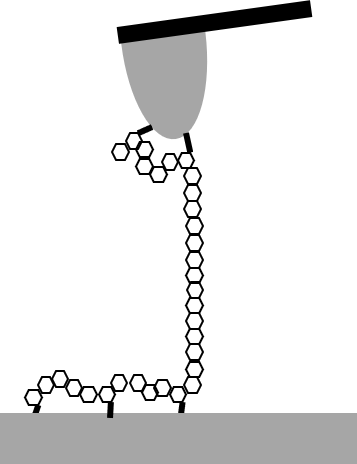
\includegraphics[width=\linewidth]{Abbildungen/Mehrfachanbindung_II.png}
	} % scalebox
	\caption[Mehrfachanbindungen]{Mehrfach angebundener \acs*{CMA}-Spacer an Substrat und \spitze.}
	\label{fig:multiple_bonding}
\end{figure}

%% Fußnotentext
\renewcommand{\noteOne}{Das Zufällig mehrere \spacer~gleichzeitig gestreckt und somit an mehreren Amidbindungen parallel gemessen wurde, kann ausgeschlossen werden. Zum einen zeigten die Kraft-Abstands-Kurven das typische Plateau von \ac{CMA} in einem Bereich von $300$ bis $400~pN$, zum aneeren zeigt die Überlagerung mehrerer Normierter Kraft-Abstands-Kurven dieser Clampereignisse keine Abweichung der mechanischen Polymereigenschaften.}


%% Ende Fußnotentext

Um im Falle eines einzelnen \ac{CMA}-Moleküls, dass über mehrere \amid~an Substrat und \spitze~gekoppelt wurde, Einzelabrisse in den Kraftkurven identifizieren zu können,  (s. Abschnitt~\ref{subsec:auflösungsgrenzen_der_kraftexperimente}) müssen die Abstände der Anbindungen groß genug sein (s.u.). Sind die Abstände zu klein überlagern sich die Einzelereignisse und abhängig von der Anzahl der vorhandenen \amide~errechnet sich so eine Geschwindigkeitskonstante, die erheblich größer ist, als sie für eine einzelne Bindung zu erwarten wäre. Wie in Abschnitt~\ref{subsec:auflösungsgrenzen_der_kraftexperimente} gezeigt wurde, liegt die Auflösungsgrenze in z-Richtung bei $\Delta l_{min} = 1~nm$. Die Monomerlänge von Amylose beträgt $l_{mono} = 0,36~nm$. Rechnerisch müssten die Amidbindungen daher mindestens 3 Monomereinheiten auseinander liegen um noch als Einzelabriss erkannt zu werden. In der Regel wurde dieser Wert durch das thermische Rauschen erhöht. Die Amplitude des thermischen Rauschens betrug im mittel ca. $40~pN$ was für typische Federkonstanten von $0,08~N~m^{-1}$ einen Wert von ca. $1~nm$ entspricht. Damit Mehrfachabrisse klar als diese erkannt werden können, sollten sie daher die doppelte Länge, also ca. $2~nm$ (6 Monomereinheiten) lang sein. Das während eines Clamp-Experiments unerkannte Mehrfachabrisse auftraten, ist hinsichtlich der langen Reaktionszeit an der Oberfläche durchaus möglich (die Wartezeit im 2. Segment betrug $3~s$). Das Zufällig mehrere \spacer~gleichzeitig gestreckt und somit mehrere Amidbindungen parallel gemessen wurden, kann ausgeschlossen werden. Zum einen zeigten die Kraft-Abstands-Kurven das typische Plateau von \ac{CMA} bei $300$ bis $400~pN$, zum anderen zeigt die Überlagerung mehrerer normierter Kraft-Abstands-Kurven dieser Clampereignisse keinen Unterschied in den mechanischen Eigenschaften (s. Anhang~\ref{appendix:A}). Die quantitative Bestimmung der mechanischen Eigenschaften nach dem Modell der frei verbundenen Kette unterstützt diese Aussage (s. Anhang~\ref{appendix:B}).\\
 Ein weiterer Effekt, der die Amidhydrolyse beeinflusste, war der thermische Drift. Dieser schwankte zwischen $1~pN~s^{-1}$ und $5~pN~s^{-1}$. Die Zeit, bis die Amidbindung auf ca. $800~pN$ gestreckt wurde betrug ca. $4~s$. Die eingestellte Kraft schwankte dadurch zwischen $600$ und $800~pN$. Beides zusammen, das Messen von Mehrfachanbindungen und eine stark schwankende Clamp-Kraft, führte bei einigen Force-Clamp-Experimenten zu einer Überschätzung der Amidbindung, wodurch die lange mittlere Lebensdauer ($\tau \approx 20~s$) des langsamen Prozesses erklärt werden kann.\\

Der schnelle Prozess mit $k_1$ stellt die Hydrolyse zur Amidbindung dar. Im basischen Bereich (pH = 8) ist $k_1^8~=~5,3~s^{-1}$ und somit größer im Vergleich zu $k_1^{7,4}~=~4,1~s^{-1}$. Die mittlere Lebensdauer sinkt von $\tau_1^{7,4}~=~0,24~s$ auf $\tau_1^8~=~0,19~s$. Dies steht im Einklang mit \cite{Smith.1998,Bundgaard.1991,Song.2000}. Hier wurde ab einem pH-Wert von ca. 8 ebenfalls eine Beschleunigung der Amidhydrolyse beobachtet. \\
Der gemessene Anstieg von $k_2^8$ stand jedoch im Gegensatz der Arbeitshypothese. Eine mögliche Erklärung liefert die Protonierung des Stickstoffatoms des \ac{TZP} während der Hydrolyse. Diese Reaktion scheint ein wichtiger Teilschritt des Bindungsbruchs zu sein, da er im basisch- bzw. sauer-katalysierten, sowie im neutralen Mechanismus der Amidhydrolyse auftritt  \cite{Zahn.2003,Zahn.2004,Zahn.2004b}. Es zeigt sich, dass das Stickstoffatoms der Amidbindung nach der Bildung des \ac{TZP} einen basischen Charakter aufweist und die Protonierung im alkalischen Milieu durch die Spaltung eines Wassermoleküls \enquote{erzwingen} kann. Es ist daher möglich, dass die Protonierung des Stickstoffatoms die Qualität der Abgangsgruppe - die primäre Aminogruppe am Substrat bzw. \spitze~- erheblich verbessert. Möglicherweise wird diese Protonierung erst ab einem pH-Wert über 8 verhindert, sodass die Geschwindigkeitsverminderung  der Hydrolyse erst bei deutlich höheren pH-Werten als pH~	8 in Erscheinung tritt.\\

%% Fußnotentext
\renewcommand{\noteOne}{Unter der Voraussetzung der mehrfach angebundenen \spacer~nach \abb~\ref{fig:multiple_bonding}.}

\renewcommand{\noteTwo}{In den Standard Kopplungsprotokollen werden i.a. Konzentration der zu koppelnden Verbindungen im mM Bereich verwendet. So z.B. in den Arbeiten von J.M. Nico \textit{et al.} \cite{Fischer.2010} oder Y. Nojima \textit{et al.} \cite{Nojima.2009}.}

\renewcommand{\noteThree}{Die Bildung der Amidbindung über die Aminolyse der \ac{NHS}-Ester läuft analog zur Rückreaktion der Amidhydrolyse \cite[10828]{Montalbetti.2005}.}
%% Ende Fußnotentext

Analog verhielt es sich mit dem langsamen Prozess. So ist $k_2^{7,4} = 0,06~s^{-1}$ auf $k_2^8 = 0,12~s^{-1}$ erhöht. Die mittlere Lebensdauer sank dabei von $\tau_2^{7,4} = 18,18~s^{-1}$ auf $\tau_2^8 = 8,33~s^{-1}$. Diese Verhalten passte zu der Vermutung der Mehrfachanbindung eines einzelnen \spacer~an Substrat und \spitze~wie sie in \abb~\ref{fig:multiple_bonding} dargestellt werden. Die Beschleunigung der Hydrolyse trat bei allen gebildeten Amidbindungen in gleichem Maße auf, somit war eine Beeinflussung der Summe aller seriell brechender Amidbindungen, unter der Annahme einzelner mehrfach angebundener \spacer, ebenfalls plausibel.\\
Im sauren pH Bereich (pH = 4,5) war die Datenlage anders. Erwartet wurde eine Beschleunigte Reaktionsgeschwindigkeit der Hydrolyse für den schnellen Prozess (ähnlich wie im basischen Bereich $k_1^{4,5} > k_1^{7,4}$), dies konnte jedoch nicht beobachtet werden. Da die Anzahl der gemessenen Überlebenszeiten mit $N_{0,2}^{4,5} = 2$ verglichen mit den anderen Zahlen ($N_{0,2}^{7,4} = 7$ und $N_{0,2}^8 = 5$), gering ausfiel, war der schnelle Prozess für pH 4,5 nur im Ansatz zu erkennen. Der Wert für $k_1^{4,5} $ mit $2,7~s^{-1}$ hatte daher keine sinnvolle Aussagekraft.\\
Der langsame Prozess bei pH 4,5 verlief etwas schneller als der langsame Prozess bei pH 7,4 ($k_2^{4,5} = 0,08~s^{-1} > k_2^{7,4} = 0,06~s^{-1}$). Die Bildung von Amidbindungen zwischen den aktivierten \carboxys~des \spacers~und den Aminogruppen auf Substrat und \spitze~haben die höchste Ausbeute in einem pH-Bereich zwischen 7 und 9 \cites{Hayworth}[69]{Fischer.2010}{Nojima.2009}. Unter pH 7 nimmt die Reaktionsfähigkeit der \ac{NHS}-Ester ab, da immer mehr freie \aminos~protoniert vorliegen und somit kein freies Elektronenpaar mehr besitzen. Oberhalb von pH 9 wird die Kopplungsreaktion durch die Instabilität des \ac{NHS}-Esters begrenzt. Aufgrund dieser Aussage während bei einem pH-Wert von 4,5 nur wenig Clampereignisse aufgrund der geringen Kopplungseffizienz zu erwarten gewesen. In den Ergebnissen waren fast ausschließlich Clampereignisse im langsamen Prozess gemessen worden, was jedoch für eine hohe Kopplungseffizienz sprach\footnote{\noteOne} sprach. Der hohe Anteil an Kategorie B Kraftkurven, sowie Clampereignisse der Kategorie D, sprechen ebenfalls für eine hohe Kopplungseffizienz (vgl. Abschnitt~\ref{kap:ergebnisse}).\\
Eine Erklärung hierfür liefert die Art und Weise, wie alle Force-Clamp-Experimente durchgeführt wurden. Während des 2. Segments (Ruhezeit) wurden die freien \aminos~von Substrat bzw. \spitze~mit den aktivierten \carboxys~am \spacer~in räumliche Nähe gebracht. Somit war die lokale Konzentration von Amino- und \carboxys~sehr hoch\footnote{\noteTwo}. Die Wahrscheinlichkeit das sich eine zufällig zurück gebildete $NH_2$-Gruppe in direkter Nähe zu einem \ac{NHS}-Ester befindet damit ebenfalls hoch. Zusammen mit der Tatsache, dass die Bildung einer Amidbindung über einen \ac{NHS}-Ester auch im sauren katalysiert wird (über Addition eines \ch{H+} an das Carbonylsauerstoff\footnote{\noteThree}) \cite[10828]{Montalbetti.2005} lässt den obigen Schluss zu.\\

Der langsame Prozess bei pH 8 verlief sehr viel schneller als der langsame Prozess bei pH 4,5 ($k_2^8 = 0,11~s^{-1} >> k_2^{4,5} = 0,08~s^{-1}$). Diese Beobachtung lässt sich ebenfalls über die erhöhte Effizienz bei der Bildung der \amid, zusammen mit einzelnen, mehrfach angebundene \spacer~erklären. Neben den oben genannten räumlichen Bedingungen spielen vor allem drei Punkte eine Rolle. 

\begin{itemize}
	\item Im basischen Milieu werden \ac{NHS}-Ester durch die Reaktion mit \ch{OH-}-Ionen gespalten \cite[289]{Latscha.2016}
	\item Im sauren Milieu stehen, wegen der Protonierung der \aminos~(\ch{R-NH3^+}), nur wenig freie Elektronenpaare zur Bildung der Amidbindung zur Verfügung \cite[189]{Latscha.2016}
	\item Zusätzlich ist der Carbonylsauerstoff der \ac{NHS}-Ester im sauren Milieu	 protoniert, daher kann der Carbonylkohlenstoff besser durch nukleophile Teilchen angegriffen werden \cite[288]{Latscha.2016}
\end{itemize}

Im basischen Milieu konkurriert die Spaltung der \ac{NHS}-Ester durch \ch{OH-}-Ionen mit der Spaltung durch \aminos. Diese Konkurrenzsituation vermindert die Ausbaute an \amide. Im sauren Milieu hingegen verhindert die Protonierung der \aminos~eine Bildung von \amide. Die Protonierung läuft als Gleichgewichtsreaktion ab \cite[189]{Latscha.2016}:

\[	\ch{R-NH2 + H3O^+ <=>> R-NH3^+ + H2O}	\]

Bei pH 4,5 liegt das Gleichgewicht zwar auf der rechten Seite, in geringem Maße bilden sich jedoch vereinzelt Aminogruppen mit freiem Elektronenpaar zurück. Hinzu kommt, dass der Angriff der verbleibenden, nicht protonierten \aminos~durch den Einsatz von Säuren katalysiert werden kann. Die Katalyse basiert, wie bei der sauren Amidhydrolyse, auf der Protonierung des Carbonylsauerstoffs. Trotz der wenigen, im sauren nicht protonierten \aminos, können sich daher im 2. Segment (Ruhezeit) tendenziell mehr \amide~bilden, als im basischen Milieu. Ein \spacer~würde dementsprechend über mehr Amidbindungen an Substrat bzw. \spitze~gekoppelt. Die Konsequenz daraus ist, dass während dem 5. Segment (Clamp) im sauren mehr \amide~brechen müssen als im basischen und daher  $k_2^{8} = 0,12~s^{-1}$ eine Größenordnung über $k_2^{4,5} = 0,08~s^{-1}$ lag.
	\chapter{Fazit}
\label{kap:Fazit}

Mehrfachanbindungen eines einzelnen \ac{CMA}-Moleküls an Substrat und \spitze~(s. \abb~\ref{fig:multiple_bonding}) konnten den langsamen Prozess bei allen pH-Werten erklären. Durch räumliche Nähe der \spitze~zum Substrat (und damit Amino- und \carboxys) sowie die Wartezeit im 2. Segment führten zu einer vermehrten Bildung von \amide~bei allen pH-Werten. Im Vergleich von pH 8 zu pH 7,4 zeigt sich eine stärkere Bildung von \amide, dass weniger Clampereignisse im schnellen Prozess zu finden waren. Die Konkurrenzreaktion der \ch{OH-}-Ionen mit den \ac{NHS}-Estern bei pH 8 sorgte jedoch dafür, dass ausreichend Clampereignisse zur Ermittlung von $k_1^8$ in den schnellen Prozess fielen.\\

Bei pH 4,5 stand der Ausbildung von \amide~die protonierte Form der \aminos~entgegen. Die Protonierung der \aminos~läuft als Gleichgewichtsreaktion ab \cite[189]{Latscha.2016}. Im sauren Milieu liegt das Gleichgewicht auf der rechten Seite. Die Carbonylgruppe der \ac{NHS}-Ester liegt ebenfalls protoniert vor. Ein nukleophiler Angriff nicht protonierter \aminos~kann deshalb viel schneller erfolgen. Zusammen mit der hohen lokalen Konzentration aller Reaktionspartner und ausreichend Reaktionszeit im 2. Segment, konnten trotz des geringen Anteils an \aminos~mit freiem Elektronenpaar, im sehr effektiv \amide~gebildet werden. Durch einzelne, mehrfach angebundene \spacer~waren daher deutlich mehr Clampereignisse im langsamen Prozess vorhanden.\\

Die Ergebnisse stützten somit nicht die Arbeitshypothese, die Hydrolyse der Amidbindung verläuft mit steigendem pH-Wert langsamer. Zumindest bei den pH-Werten 7,4 und 8 verhielt sich die Hydrolysegeschwindigkeit der Amidbindung unter Einfluss einer äußeren Kraft wie in \cite{Smith.1998,Bundgaard.1991,Song.2000} beschrieben, jedoch um den Faktor $10^9$ beschleunigt. Bei einem pH-Wert von 4,5 konnte über die einzelne Amidbindung keine Aussage getroffen werden. Hier wurden hauptsächlich mehrere, hintereinander brechende Amidbindungen gemessen. Diese hintereinander abreißenden Bindungen konnten aufgrund des vorliegenden Messaufbaus nicht voneinander unterschieden werden. Wurden die langsamen Prozesse bei pH 7,4 und 4,5 miteinander vergleichen($k_2^{7,4} = 0,06~s^{-1}$ bzw. $k_2^{4,5} = 0,08~s^{-1}$), konnte auch hier eine Beschleunigung der Hydrolysegeschwindigkeit der Amidbindung festgestellt werden.




	\chapter{Ausblick}
\label{kap:ausblick}

Obwohl die Kopplungschemie über \ac{NHS}/\ac{EDC} standardmäßig in einem engen pH-Bereich von 7 bis 9 stattfindet \cite{Hayworth,Fischer.2010,Nojima.2009}, konnte durch die spezielle Charakteristik der Force-Clamp-Versuche der pH-Bereich auf 4,5 bis 9 erweitert werden. Dabei werden Abtastspitze und Substrat auf eine Kraft von $250~pN$ zusammengebracht und über einen Zeitraum von $3~s$ ruhen gelassen (2. Segment). Somit waren alle Reaktionspartner in räumlicher Nähe zueinander und hatten genügend Zeit miteinander zu reagieren. Um die störenden Mehrfachanbindungen eines CMA-Moleküls an Abtastspitze und Substrat zu minimieren stellen die Haltekraft und Ruhezeit im 2. Segment somit die wichtigsten Parameter dar. In wie fern bei niedrigeren pH-Werten als 4,5 gemessen werden kann muss erst getestet werden. Fischer et al. \cite{Fischer.2010} spricht von einem pH-Wert von 3,5 als Grenze. Wobei diese Grenze für Force-Clamp-Experimente nicht zwingend gelten muss. Wie die erhaltenen Messergebnisse bei pH 4,5 zeigen, sollte durch herkömmlichen Kopplungsprotokolle keine nennenswerte Ausbildung von Amidbindungen stattfinden. Bei den durchgeführten Force-Clamp-Experimenten war die Ausbeute von Clampereignisse im niedrigen pH-Bereich am höchsten (vgl. \abb~\ref{fig:general_curve_composition} und \ref{fig:discarded_curve_composition}). Somit wäre die Messung der Amidbindung unterhalb von pH 3,5 mittels einer \ac{EDC}/\ac{NHS}-Kopplung möglich. Bei einem pH-Wert von 9 liegt die mittlere Lebensdauer der NHS-Ester bei wenigen Minuten \cite{Hayworth}. Dies macht die Überprüfung der Arbeitshypothese bei einem pH-Wert von über 9 schwierig. Es wäre denkbar für solche pH-Werte andere Methoden zur Bildung der Amidbindung zu verwenden. Ein Beispiel hierfür wäre die Kopplung von primären Aminen mit Carbonsäurehalogeniden wie sie in \cite{Montalbetti.2005} beschrieben wird.
	%---------------------------Ende der Kapitelliste------------------
	
	
	%--------------------print Bibliography at the end--------------
	\renewcommand{\leftmark}{Referenzen} % Setzt entsprechende section wieder in die Kopfzeile (linke Seite)
	\renewcommand{\refname}{Referenzen} % Setzt entsprechende section wieder in die Kopfzeile (rechteSeite)
	\renewcommand{\section}[2]{}
	\printbibliography
	
	%----------------------------------Abkürzungen----------------------
	\chapter*{Abkürzungsverzeichnis}
	\begin{acronym}[längste Abkürzungen]
		\acro{AFM}{Atomic Force Microscope}
		\acro{CMA}{\iupac{Carboxy|methyl|amylose}}
		\acro{DLC}{Diamond Like Carbon}
		\acro{DP}[\textit{DP}]{Doppelpeak}
		\acro{EDC}{\iupac{1-Ethyl-3-(3-di|methyl|amino|propyl) Carbo|diimid Hydro|chlorid}}
		\acro{HCl}[\ch{HCl}]{Salzsäure}
		\acro{HDC}{High Densitiy Carbon}
		\acro{NaOH}[\ch{NaOH}]{Natriumhydroxid}
		\acro{NHS}{\iupac{N-Hydroxy|succinimid}}
		\acro{PBS}[\ch{PBS}]{Phosphate Buffered Saline}
		\acro{SMFS}{Single Molecule Force Spectroscopy}
		\acro{tmax}[t$_\mathrm{max}$]{Maximale Clamptzeit}
		\acro{TZP}{Tetraedisches Zwischenprodukt}
		\acro{ZI}{Zwitterion}
		\acro{UZ}[ÜZ]{Übergangszustand}
	\end{acronym}
	
	%TODO: In Anhang: Überlagerung von normierten Clampereignissen zeigen (für diskussion der Mehrfachanbindung)
	
	%TODO: In Anhang: FLC-Fits mehrerer Clampereignisse im unteren Kraftbereich, um zu zeigen, dass mechanische Eigenschaften der Polymere an denen gemessen wurden gleich sind.
	
	%%% Einfügen eines Anhangs
	\appendix
	
\end{document}
